\documentclass{beamer}

% xcolor and define colors -------------------------
\usepackage{xcolor}

% https://www.viget.com/articles/color-contrast/
\definecolor{purple}{HTML}{5601A4}
\definecolor{navy}{HTML}{0D3D56}
\definecolor{ruby}{HTML}{9a2515}
\definecolor{alice}{HTML}{107895}
\definecolor{daisy}{HTML}{EBC944}
\definecolor{coral}{HTML}{F26D21}
\definecolor{kelly}{HTML}{829356}
\definecolor{cranberry}{HTML}{E64173}
\definecolor{jet}{HTML}{131516}
\definecolor{asher}{HTML}{555F61}
\definecolor{slate}{HTML}{314F4F}

% Mixtape Sessions
\definecolor{picton-blue}{HTML}{00b7ff}
\definecolor{violet-red}{HTML}{ff3881}
\definecolor{sun}{HTML}{ffaf18}
\definecolor{electric-violet}{HTML}{871EFF}

% Main theme colors
\definecolor{accent}{HTML}{00b7ff}
\definecolor{accent2}{HTML}{871EFF}
\definecolor{gray100}{HTML}{f3f4f6}
\definecolor{gray800}{HTML}{1F292D}


% Beamer Options -------------------------------------

% Background
\setbeamercolor{background canvas}{bg = white}

% Change text margins
\setbeamersize{text margin left = 15pt, text margin right = 15pt} 

% \alert
\setbeamercolor{alerted text}{fg = accent2}

% Frame title
\setbeamercolor{frametitle}{bg = white, fg = jet}
\setbeamercolor{framesubtitle}{bg = white, fg = accent}
\setbeamerfont{framesubtitle}{size = \small, shape = \itshape}

% Block
\setbeamercolor{block title}{fg = white, bg = accent2}
\setbeamercolor{block body}{fg = gray800, bg = gray100}

% Title page
\setbeamercolor{title}{fg = gray800}
\setbeamercolor{subtitle}{fg = accent}

%% Custom \maketitle and \titlepage
\setbeamertemplate{title page}
{
    %\begin{centering}
        \vspace{20mm}
        {\Large \usebeamerfont{title}\usebeamercolor[fg]{title}\inserttitle}\\
        {\large \itshape \usebeamerfont{subtitle}\usebeamercolor[fg]{subtitle}\insertsubtitle}\\ \vspace{10mm}
        {\insertauthor}\\
        {\color{asher}\small{\insertdate}}\\
    %\end{centering}
}

% Table of Contents
\setbeamercolor{section in toc}{fg = accent!70!jet}
\setbeamercolor{subsection in toc}{fg = jet}

% Button 
\setbeamercolor{button}{bg = accent}

% Remove navigation symbols
\setbeamertemplate{navigation symbols}{}

% Table and Figure captions
\setbeamercolor{caption}{fg=jet!70!white}
\setbeamercolor{caption name}{fg=jet}
\setbeamerfont{caption name}{shape = \itshape}

% Bullet points

%% Fix left-margins
\settowidth{\leftmargini}{\usebeamertemplate{itemize item}}
\addtolength{\leftmargini}{\labelsep}

%% enumerate item color
\setbeamercolor{enumerate item}{fg = accent}
\setbeamerfont{enumerate item}{size = \small}
\setbeamertemplate{enumerate item}{\insertenumlabel.}

%% itemize
\setbeamercolor{itemize item}{fg = accent!70!white}
\setbeamerfont{itemize item}{size = \small}
\setbeamertemplate{itemize item}[circle]

%% right arrow for subitems
\setbeamercolor{itemize subitem}{fg = accent!60!white}
\setbeamerfont{itemize subitem}{size = \small}
\setbeamertemplate{itemize subitem}{$\rightarrow$}

\setbeamertemplate{itemize subsubitem}[square]
\setbeamercolor{itemize subsubitem}{fg = jet}
\setbeamerfont{itemize subsubitem}{size = \small}


% Special characters

\usepackage{collectbox}

\makeatletter
\newcommand{\mybox}{%
    \collectbox{%
        \setlength{\fboxsep}{1pt}%
        \fbox{\BOXCONTENT}%
    }%
}
\makeatother





% Links ----------------------------------------------

\usepackage{hyperref}
\hypersetup{
  colorlinks = true,
  linkcolor = accent2,
  filecolor = accent2,
  urlcolor = accent2,
  citecolor = accent2,
}


% Line spacing --------------------------------------
\usepackage{setspace}
\setstretch{1.1}


% \begin{columns} -----------------------------------
\usepackage{multicol}


% Fonts ---------------------------------------------
% Beamer Option to use custom fonts
\usefonttheme{professionalfonts}

% \usepackage[utopia, smallerops, varg]{newtxmath}
% \usepackage{utopia}
\usepackage[sfdefault,light]{roboto}

% Small adjustments to text kerning
\usepackage{microtype}



% Remove annoying over-full box warnings -----------
\vfuzz2pt 
\hfuzz2pt


% Table of Contents with Sections
\setbeamerfont{myTOC}{series=\bfseries, size=\Large}
\AtBeginSection[]{
        \frame{
            \frametitle{Roadmap}
            \tableofcontents[current]   
        }
    }


% Tables -------------------------------------------
% Tables too big
% \begin{adjustbox}{width = 1.2\textwidth, center}
\usepackage{adjustbox}
\usepackage{array}
\usepackage{threeparttable, booktabs, adjustbox}
    
% Fix \input with tables
% \input fails when \\ is at end of external .tex file
\makeatletter
\let\input\@@input
\makeatother

% Tables too narrow
% \begin{tabularx}{\linewidth}{cols}
% col-types: X - center, L - left, R -right
% Relative scale: >{\hsize=.8\hsize}X/L/R
\usepackage{tabularx}
\newcolumntype{L}{>{\raggedright\arraybackslash}X}
\newcolumntype{R}{>{\raggedleft\arraybackslash}X}
\newcolumntype{C}{>{\centering\arraybackslash}X}

% Figures

% \imageframe{img_name} -----------------------------
% from https://github.com/mattjetwell/cousteau
\newcommand{\imageframe}[1]{%
    \begin{frame}[plain]
        \begin{tikzpicture}[remember picture, overlay]
            \node[at = (current page.center), xshift = 0cm] (cover) {%
                \includegraphics[keepaspectratio, width=\paperwidth, height=\paperheight]{#1}
            };
        \end{tikzpicture}
    \end{frame}%
}

% subfigures
\usepackage{subfigure}


% Highlight slide -----------------------------------
% \begin{transitionframe} Text \end{transitionframe}
% from paulgp's beamer tips
\newenvironment{transitionframe}{
    \setbeamercolor{background canvas}{bg=accent!40!black}
    \begin{frame}\color{accent!10!white}\LARGE\centering
}{
    \end{frame}
}


% Table Highlighting --------------------------------
% Create top-left and bottom-right markets in tabular cells with a unique matching id and these commands will outline those cells
\usepackage[beamer,customcolors]{hf-tikz}
\usetikzlibrary{calc}
\usetikzlibrary{fit,shapes.misc}

% To set the hypothesis highlighting boxes red.
\newcommand\marktopleft[1]{%
    \tikz[overlay,remember picture] 
        \node (marker-#1-a) at (0,1.5ex) {};%
}
\newcommand\markbottomright[1]{%
    \tikz[overlay,remember picture] 
        \node (marker-#1-b) at (0,0) {};%
    \tikz[accent!80!jet, ultra thick, overlay, remember picture, inner sep=4pt]
        \node[draw, rectangle, fit=(marker-#1-a.center) (marker-#1-b.center)] {};%
}

\usepackage{breqn} % Breaks lines

\usepackage{amsmath}
\usepackage{mathtools}

\usepackage{pdfpages} % \includepdf

\usepackage{listings} % R code
\usepackage{verbatim} % verbatim

% Video stuff
\usepackage{media9}

% packages for bibs and cites
\usepackage{natbib}
\usepackage{har2nat}
\newcommand{\possessivecite}[1]{\citeauthor{#1}'s \citeyearpar{#1}}
\usepackage{breakcites}
\usepackage{alltt}

% Setup math operators
\DeclareMathOperator{\E}{E} \DeclareMathOperator{\tr}{tr} \DeclareMathOperator{\se}{se} \DeclareMathOperator{\I}{I} \DeclareMathOperator{\sign}{sign} \DeclareMathOperator{\supp}{supp} \DeclareMathOperator{\plim}{plim}
\DeclareMathOperator*{\dlim}{\mathnormal{d}\mkern2mu-lim}
\newcommand\independent{\protect\mathpalette{\protect\independenT}{\perp}}
   \def\independenT#1#2{\mathrel{\rlap{$#1#2$}\mkern2mu{#1#2}}}
\newcommand*\colvec[1]{\begin{pmatrix}#1\end{pmatrix}}

\newcommand{\myurlshort}[2]{\href{#1}{\textcolor{gray}{\textsf{#2}}}}


\begin{document}

\imageframe{./lecture_includes/mixtape_did_cover.png}


% ---- Content ----



\section{Diff-in-Diff with a Designed Checklist}


\subsection{Managing expectations}


\begin{frame}{Introduction}

\begin{itemize}
\item Thank you coming to Mixtape Sessions' Causal Inference 2 workshop on difference-in-differences!  
\item Scott Cunningham, Ben H. Williams Professor of Economics at Baylor University in Texas USA
\item 9:00am to 5:00pm CST, 15 min breaks every hour, 1 hour lunch at 12:00
\item Lecture, discussion, exercises, application with "live coding" exercises
\end{itemize}

\end{frame}


\begin{frame}{What my pedagogy is like}

\begin{itemize}
\item High energy, eclectic approach to teaching
\item Move between the econometrics, history of thought, videos, applications, code, spreadsheets, exercises
\item Workshop is intended to take someone from knowing nothing about difference-in-differences to a broad level of competency on advanced topics
\item Ask questions at any point; I'll do my best to answer them but will sometimes defer it to the break
\end{itemize}

\end{frame}


\begin{frame}{Class goals}
Pedagogical goal is to break down the procedures into plain English, rebuilding it into something you can and want to use, but also:

  \begin{enumerate}
    \item \textbf{Confidence}: You will feel like you have a good enough understanding of diff-in-diff, both in its basics and some more contemporary issues, so that it seems like an intuitive and useful tool you could imagine using
    \item \textbf{Comprehension}: You will have learned a lot both conceptually and in the specifics, particularly with regards to issues around identification and estimation in the diff-in-diff 
    \item \textbf{Competency}: You will have more knowledge of programming syntax in Stata and R so that later you can apply this in your own work
  \end{enumerate}

\end{frame}

\begin{frame}{Organization of workshop}

\begin{itemize}

\item Check out Baker, Callaway, Cunningham, Goodman-Bacon and Sant'Anna (2025) in Readings
\item I'm building a workshop based on it, but centered more on a "designed checklist"
\item Hopefully you find it useful this way!
\end{itemize}

\end{frame}

\subsection{Researcher Bias, Controlled Design and the Checklist}


\begin{frame}{Different Kinds of Biased Studies}

\begin{itemize}
\item Malfeasance (e.g., data fabrication) and p-hacking have probably grown because of the high returns to top publications
\item Publication bias.  Journals may have preferences for certain results, certain people, or certain thresholds (e.g., $p$-value$<0.05$)
\item Ignorance, low quality data, poor understanding of and therefore misuse of econometric methods
\item But there's a more innocent one that I'll call non-standard errors
\end{itemize}

\end{frame}


\begin{frame}{Non-Standard Errors}

\begin{figure}
    \centering
    
\includegraphics[height=0.9\textheight]{./lecture_includes/nick_design}
\end{figure}

\end{frame}

 
\begin{frame}{Non-Standard Errors}
 
\begin{figure}
    \centering
    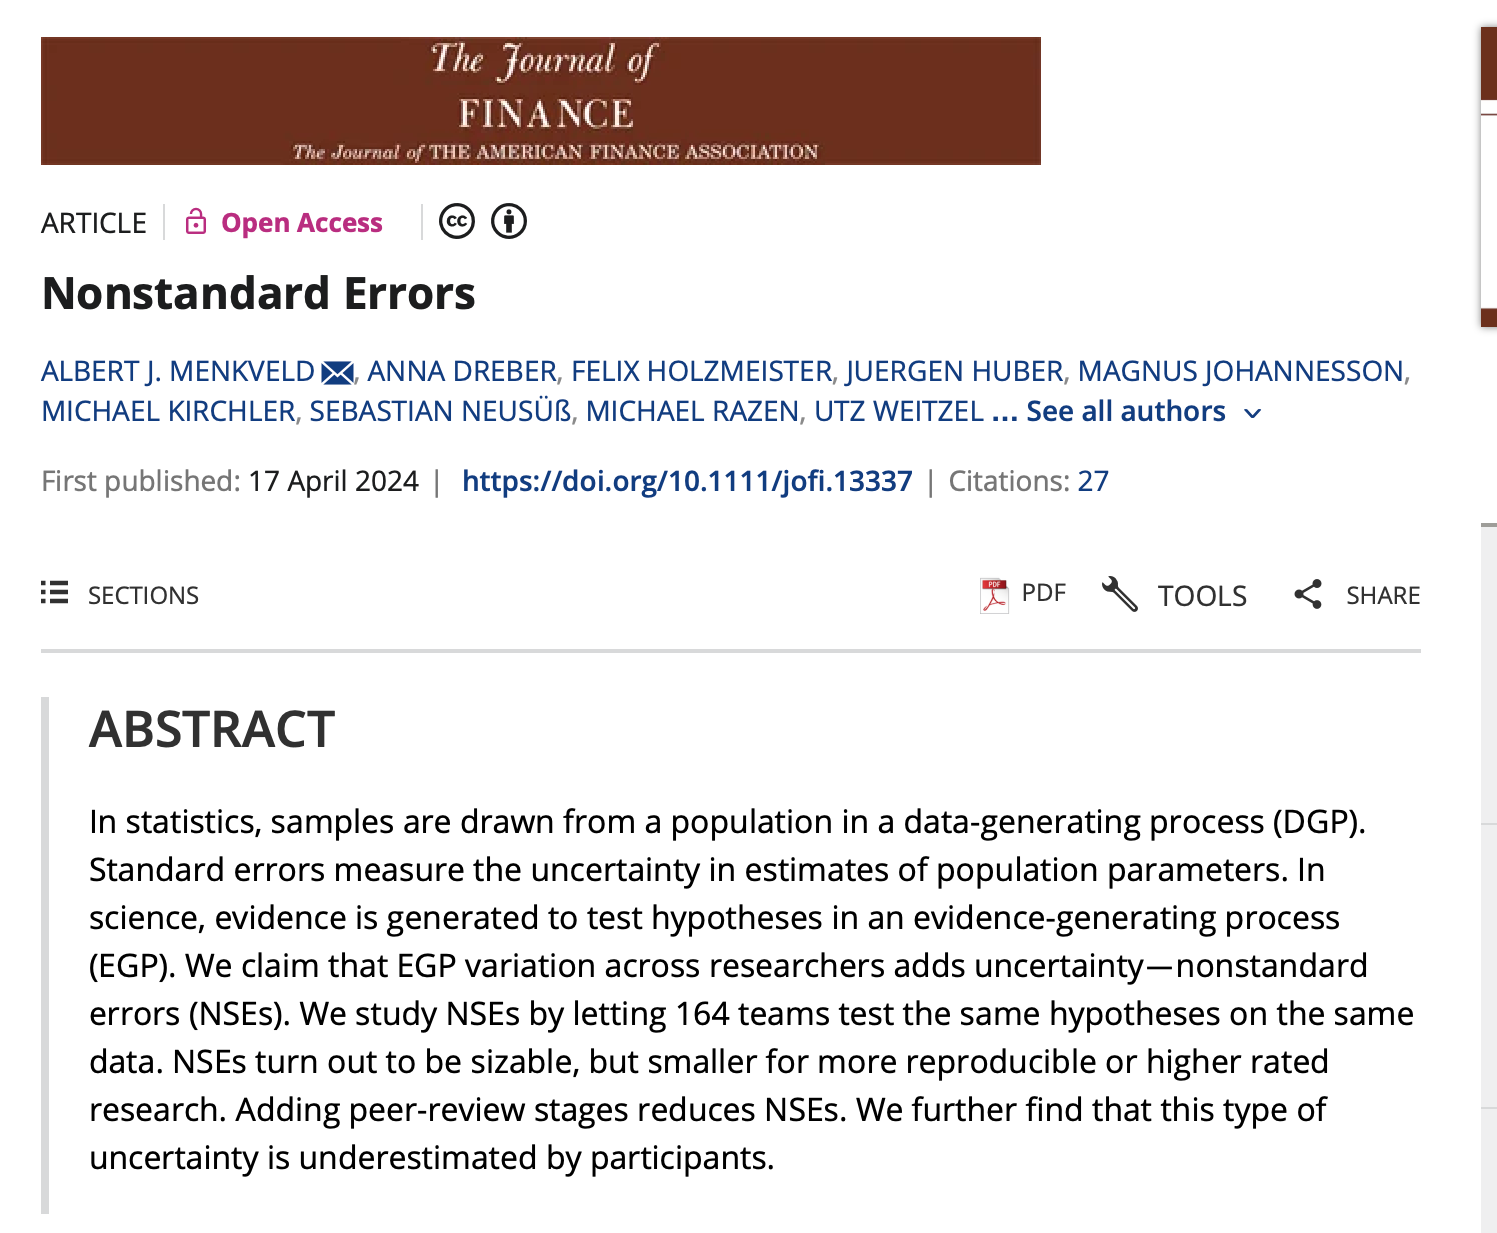
\includegraphics[height=0.9\textheight]{./lecture_includes/nonstandard_errors2}
\end{figure}

\end{frame}


\begin{frame}{Non-Standard Errors}
 
\begin{figure}
    \centering
    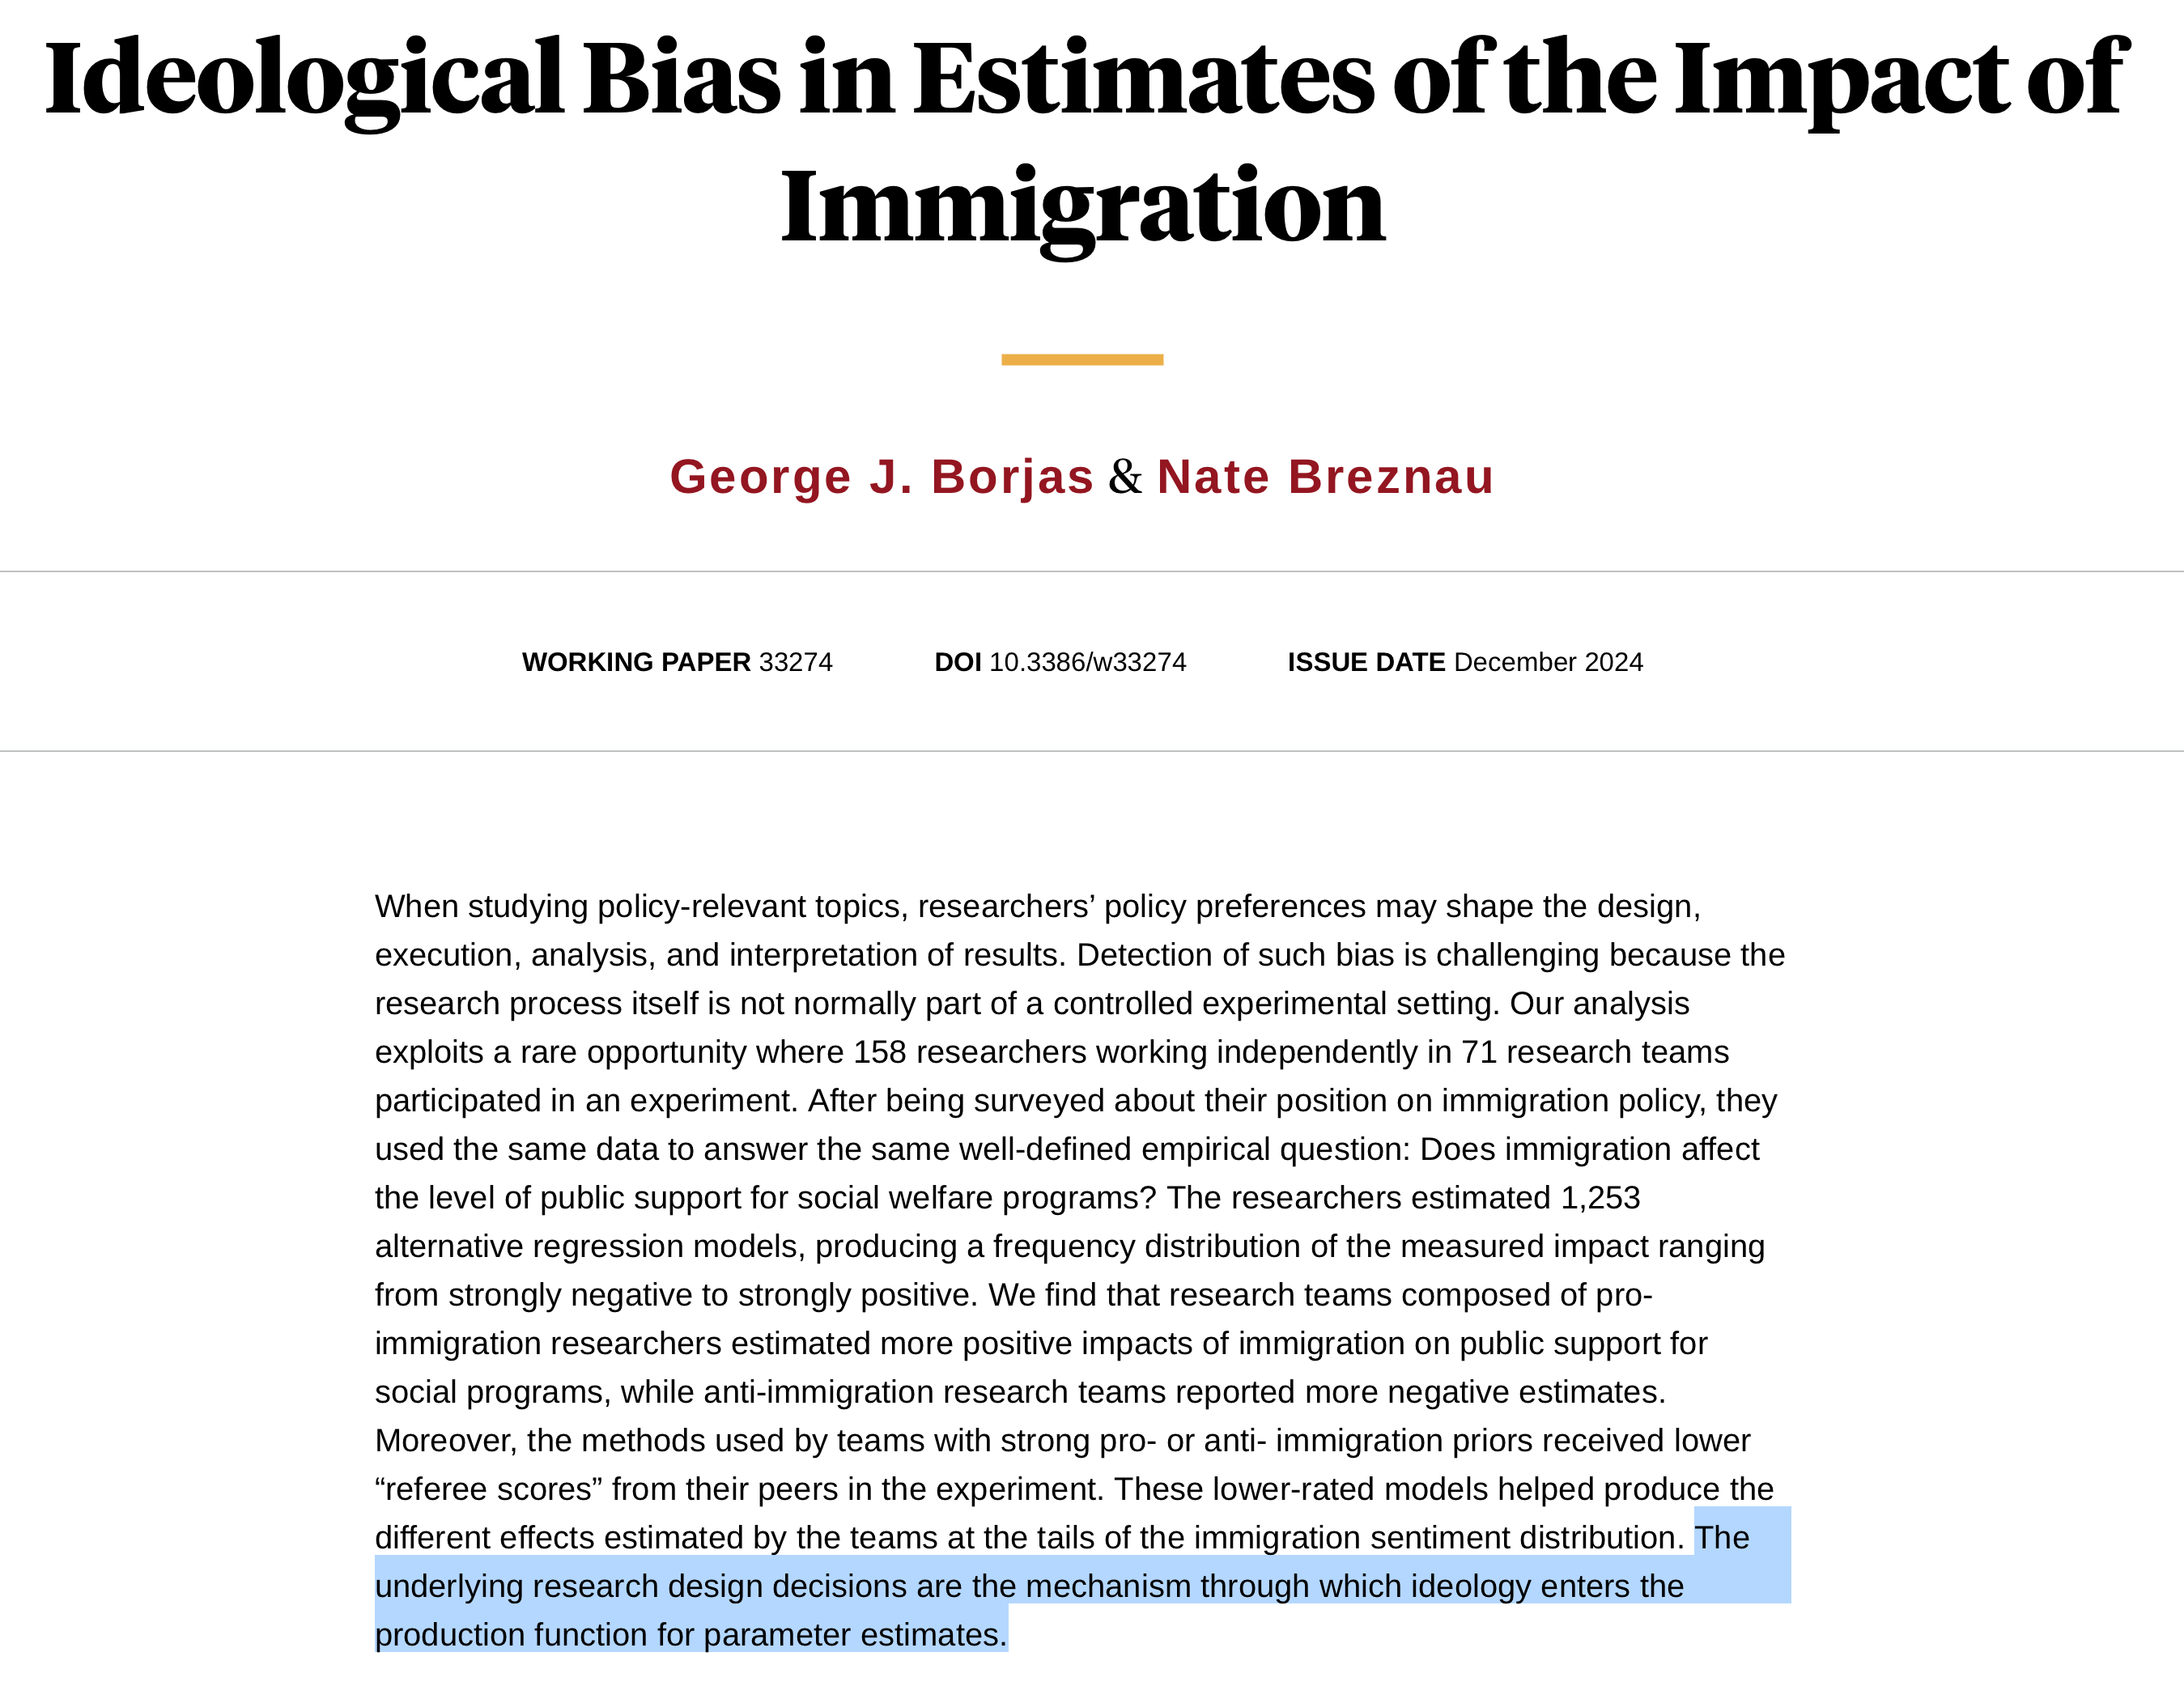
\includegraphics[height=0.9\textheight]{./lecture_includes/borjas_design}
\end{figure}

\end{frame}







\begin{frame}{Controlled Randomization}

\begin{itemize}
\item Randomized controlled trials (RCTs) are not the only design to exploit "coin flips", but the difference is they \textbf{control} the randomization 
\item But not all RCTs are the same -- some control the study extraordinarily well, some can be done so poorly that we learn nothing
\item Quasi-experimental controlled design (QCD) cannot control the randomization, but they can control the design of the study so as to mimic the RCT

\end{itemize}

\end{frame}

	 



\begin{frame}{QCD Needs More "Design Time}

\begin{itemize}
\item Think of an RCT as producing something, but what and how?
\item Well designed RCTs produce \textbf{warranted beliefs} inside humans' minds
\item Imagine then that producing warranted beliefs is a function of "well spent time" designing a study
\end{itemize}

\end{frame}


\begin{frame}{Quasi-Experimental Controlled Design (QCD)}
 
\begin{figure}
    \centering
    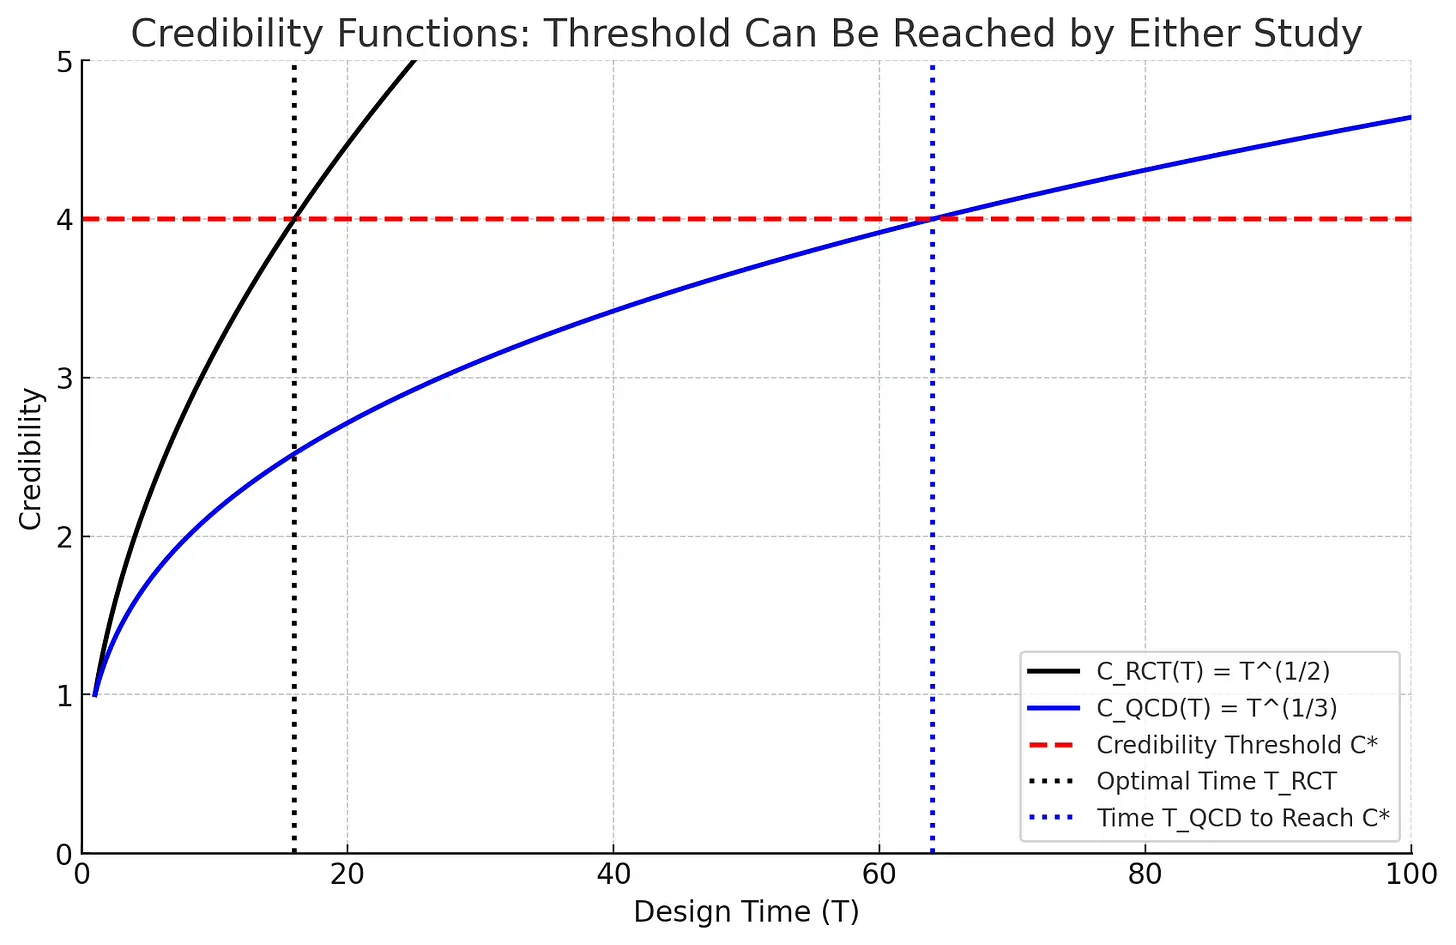
\includegraphics[width=\textwidth]{./lecture_includes/qcd}
\end{figure}

\end{frame}









\begin{frame}{Current Practices}
 
\begin{figure}
    \centering
    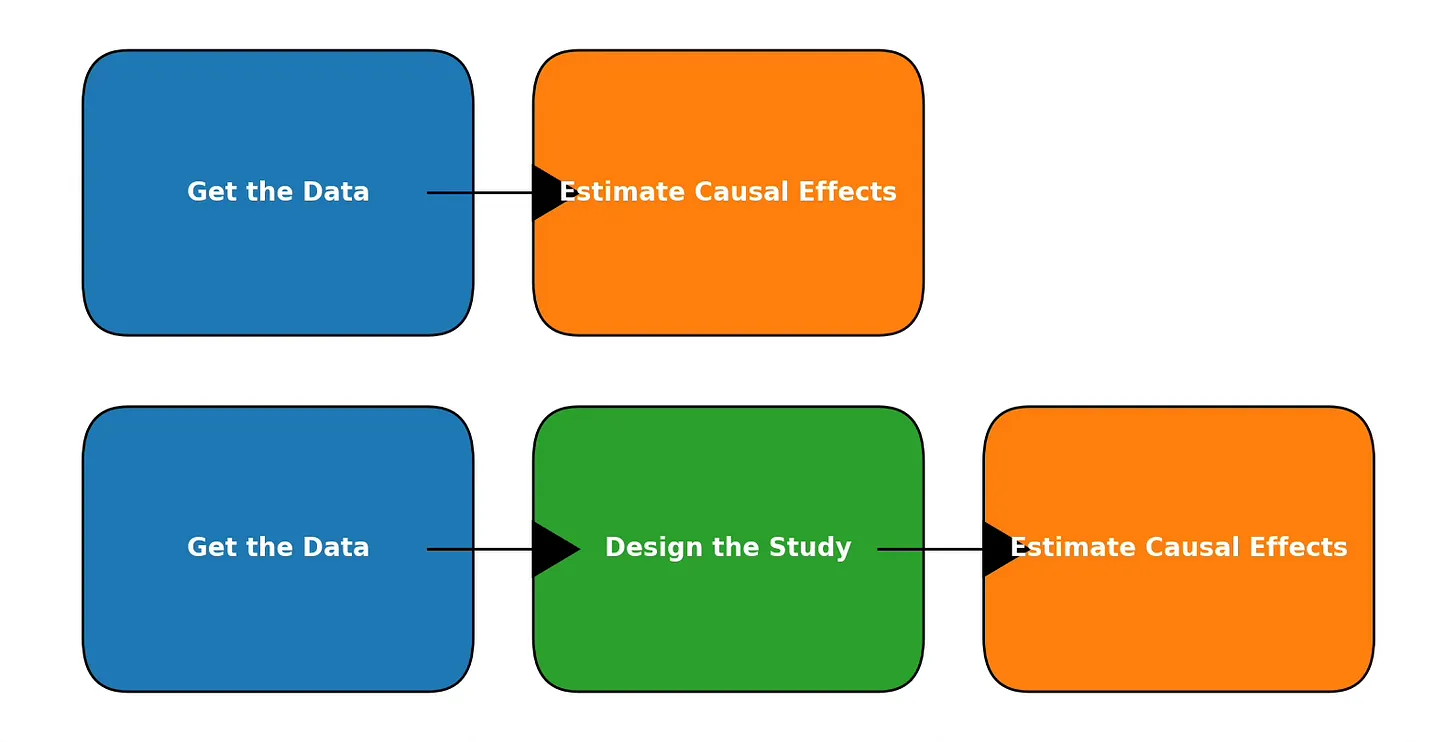
\includegraphics[width=\textwidth]{./lecture_includes/design_stage}
\end{figure}

\end{frame}


\begin{frame}{How Checklists Saved Lives in Medicine}
    \textbf{Key Idea:} Checklists reduce errors and improve patient safety by standardizing procedures and preventing overlooked steps.

    \begin{itemize}
        \item 
	\textit{The Checklist Manifesto} by Atul Gawande explores how checklists improve outcomes in medicine, aviation, and other fields.
        \item 
	The WHO Surgical Safety Checklist reduced complications and mortality in surgeries worldwide. A study found a 36\% reduction in major surgical complications.
        \item 
	Checklists are thought to work because they:
        \begin{itemize}
            \item Ensure that critical steps are not skipped.
            \item Encourage teamwork and communication.
            \item Create a structured, repeatable process for complex tasks.
        \end{itemize}
    \end{itemize}


\end{frame}

\begin{frame}{Diff-in-diff checklist}

\begin{itemize}
       \item We are going to review 14-15 hours of diff-in-diff by using the checklist as our lamp 
       \item Inspired by Pedro Sant'Anna, Guido Imbens, Roth, et al. (2022) and my own additions
	\item We'll walk through technical exposition, stories, papers, simulations and examples
	\item Hope is that this is better than simply listing everything, as if an encyclopedia of diff-in-diff, which I think can be overwhelming
\end{itemize}

\end{frame}


\subsection{Diff-in-Diff Fundamentals}

\begin{frame}{Growing popularity in economics}

	\begin{figure}
	\caption{Currie, et al. (2020)}
	\includegraphics[scale=0.25]{./lecture_includes/currie_did.png}
	\end{figure}

\bigskip

\footnotesize

With some exception (e.g., Heckman, Ichimura and Todd 1997; Abadie 2005; Bertrand, Duflo and Mullainthan 2004), econometricians had not given it much notice

\end{frame}








\begin{frame}{What is difference-in-differences (DiD)}

\begin{itemize}
\item DiD is when a group of units are assigned some treatment and then compared to a group of units that weren't before and after
\item One of the most widely used quasi-experimental methods in economics and increasingly in industry
\item Predates the randomized experiment by 80 years, but uses basic experimental ideas about treatment and control groups (just not randomized)
\item Uses panel or repeated cross section datasets, binary treatments usually, and often covariates
\item We'll do a quick run through the social history of diff-in-diff to set the stage for our workshop this week
\end{itemize}
\end{frame}








\begin{frame}{Ignaz Semmelweis and washing hands}

\begin{itemize}
\item Early 1820s, Vienna passed legislation requiring that if a pregnant women giving birth went to a public hospital (free care), then depending on the day of week and time of day, she would be routed to either the midwife wing or the physician wing (most likely resulting in random assignment)
\item But by the 1840s, Ignaz Semmelweis noticed that pregnant women died after delivery in the (male) wing at a rate of 13-18\%, but only 3\% in the (female) midwife wing -- cause was puerperal or “childbed” fever
\item Somehow this was also we known -- women would give birth in the street rather than go to the physician if they were unlucky enough to have their water break on the wrong day and time
\end{itemize}

\end{frame}

\begin{frame}{Ignaz Semmelweis and washing hands}

\begin{itemize}
\item Ignaz Semmelweis conjectures after a lot of observation that the cause is the teaching faculty teaching anatomy using cadavers and then delivering babies \emph{without washing hands}
\item New training happens to one but not the other and Semmelweis thinks the mortality is caused by working with cadavers
\item Convinced the hospital to have physicians wash their hands in chlorine but not the midwives, creating a type of difference-in-differences design 
\end{itemize}

\end{frame}

\begin{frame}{Semmelweis diff-in-diff evidence}

	\begin{figure}
	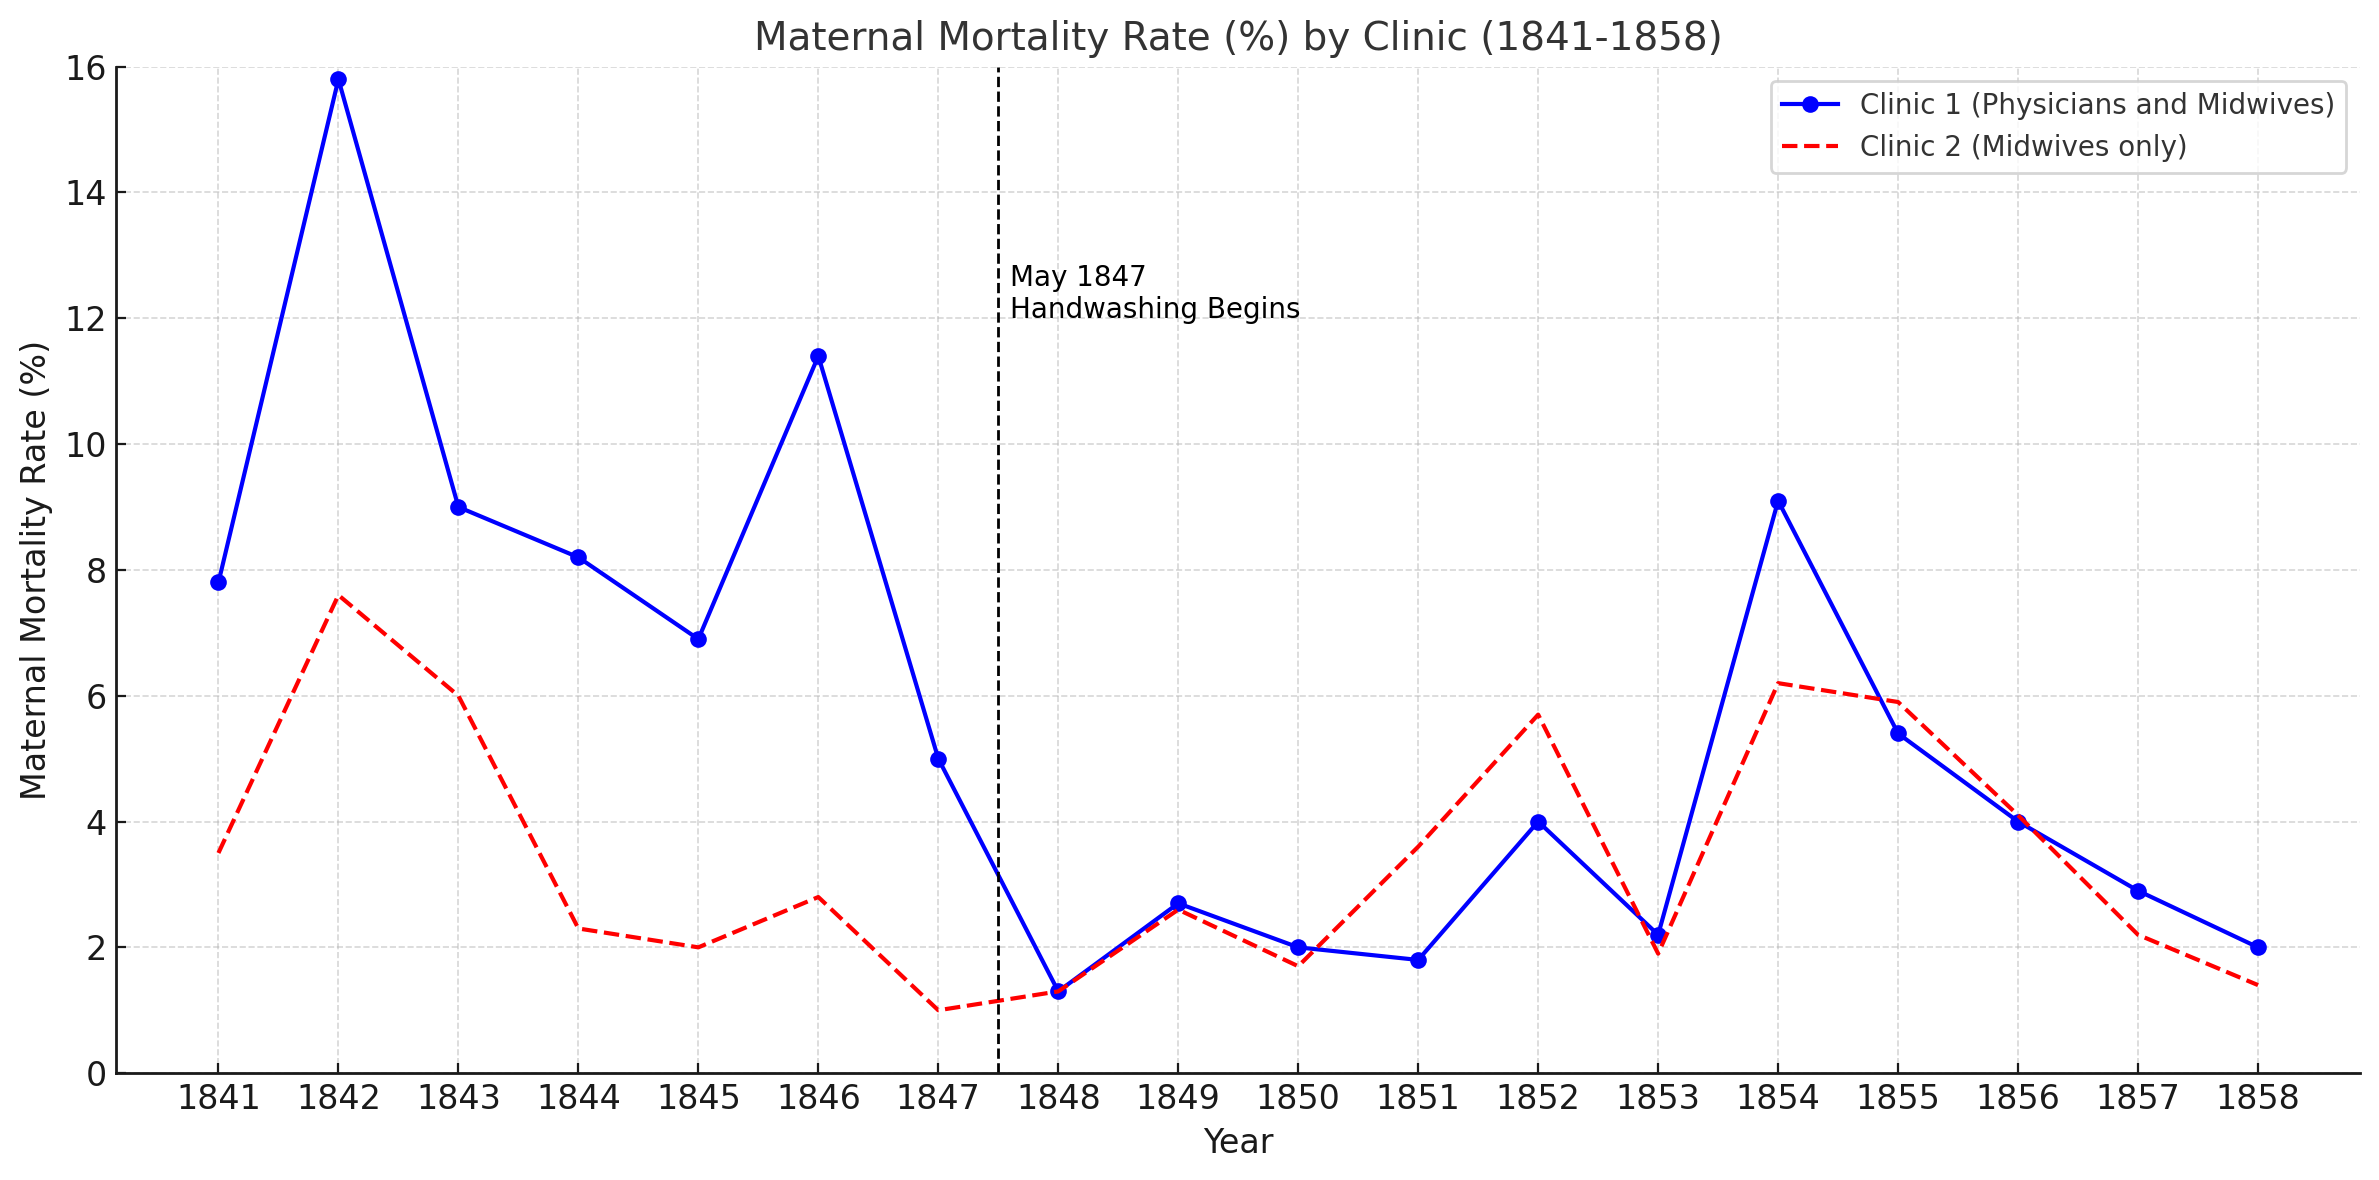
\includegraphics[scale=0.4]{./lecture_includes/semmelweis_graphic.png}
	\end{figure}


\end{frame}



\begin{frame}{John Snow and cholera}

\begin{itemize}
\item Three major waves of cholera in the early to mid 1800s in London, largely thought to be spread by miasma (``dirty air'')
\item John Snow believed cholera was spread through the Thames water supply through an invisible creature that entered the body through food and drink, caused the body to expel water, placing the creature back in the Thames and causing epidemic waves
\item London passes ordinance requiring water utility companies to move inlet pipe further up the Thames, above the city center, but not everyone complies
\item Natural experiment: Lambeth water company moves its pipe between 1849 and 1854; Southwark and Vauxhall water company delayed
\end{itemize}

\end{frame}


\begin{frame}

	\begin{figure}
	\caption{Two water utility companies in London 1854}
	\includegraphics[scale=0.225]{./lecture_includes/lambeth.png}
	\end{figure}


\end{frame}



\begin{frame}{Difference-in-differences}

\begin{table}\centering
\scriptsize
		\caption{Lambeth and Southwark and Vauxhall, 1849 and 1854}
		\begin{center}
		\begin{tabular}{lll|lc}
		\toprule
		\multicolumn{1}{l}{\textbf{Companies}}&
		\multicolumn{1}{c}{\textbf{Time}}&
		\multicolumn{1}{c}{\textbf{Outcome}}&
		\multicolumn{1}{c}{$D_1$}&
		\multicolumn{1}{c}{$D_2$}\\
		\midrule
		Lambeth & Before & $Y=L$ \\
		& After & $Y=L + L_t + D$ & $\textcolor{red}{L_t}+D$\\
		\midrule
		& & & & $D + (\textcolor{red}{L_t}- SV_t)$ \\
		\midrule
		Southwark and Vauxhall & Before & $Y=SV$ \\
		& After & $Y=SV + SV_t$ & $SV_t$\\
		\bottomrule
		\end{tabular}
		\end{center}
	\end{table}

\begin{eqnarray*}
\widehat{\delta}_{did} = D + (\textcolor{red}{L_t}- SV_t)
\end{eqnarray*}This method yields an unbiased estimate of D if $\textcolor{red}{L_t} = SV_t$, but note that $\textcolor{red}{L_t}$ is a counterfactual trend and therefore not known

\end{frame}


\begin{frame}
\begin{center}
\textbf{Two rivers into causal inference}
\end{center}

\begin{tikzpicture}[scale=0.7, every node/.style={scale=0.7}]
% Orley Ashenfelter Stream
\node at (-5,6) {\textbf{Orley Ashenfelter}};
\draw[->, thick] (-5,5.5) -- (-5,5.2);
\node at (-5,5) {Princeton Industrial Relations Section};
\draw[->, thick] (-5,4.5) -- (-5,4.2);
\node at (-5,4) {Quasi-Experimental Design};
\draw[->, thick] (-5,3.5) -- (-5,3.2);
\node at (-5,3) {David Card};
\draw[->, thick] (-5,2.5) -- (-5,2.2);
\node at (-5,2) {Alan Krueger};
\draw[->, thick] (-5,1.5) -- (-5,1.2);

% Don Rubin Stream
\node at (5,6) {\textbf{Don Rubin}};
\draw[->, thick] (5,5.5) -- (5,5.2);
\node at (5,5) {Harvard Statistics};
\draw[->, thick] (5,4.5) -- (5,4.2);
\node at (5,4) {Experimental Design};
\draw[->, thick] (5,3.5) -- (5,3.2);
\node at (5,3) {Potential Outcomes};
\draw[->, thick] (5,2.5) -- (5,2.2);
\node at (5,2) {Treatment Effects};
\draw[->, thick] (5,1.5) -- (5,1.2);

% Arrow from Orley Ashenfelter and Don Rubin streams to bottom rectangle
\draw[->, thick] (-5,1) -- (0,-0.8);
\draw[->, thick] (5,1) -- (0,-0.8);

% Bottom Rectangle
\node[draw, minimum width=8cm, minimum height=2cm, anchor=north] at (0,-0.8) {
    \begin{tabular}{c}
        Josh Angrist \\
        (Princeton)
    \end{tabular}
    \hspace{2cm}
    \begin{tabular}{c}
        Guido Imbens \\
        (Brown)
    \end{tabular}
};
\node[anchor=north] at (0,-2.8) {\textbf{Harvard Economics}};

\end{tikzpicture}

\end{frame}


\begin{frame}{Orley Ashenfelter and diff-in-diff}

\begin{itemize}

\item Diff-in-diff gets rediscovered by Orley Ashenfelter from Princeton 
\item Leaves academia to work in Washington DC to study job training programs for low skill workers
\item Coins the phrase "difference-in-differences" so as to avoid having to explain regressions to bureaucrats (3:53)  \url{https://youtu.be/WnB3EJ8K7lg?si=uE4clqUIPzvbxm0r&t=2}
\item More associated with David Card (Mariel boatlift, minimum wage), but it was earlier that he and Orley worked with the method, and ironically largely, rejected its usefulness for the questions they were working on

\end{itemize}

\end{frame}




\subsection{Potential outcomes}


\begin{frame}{Identification vs Estimation}

\begin{itemize}
\item We must start by making a distinction between the parameter we are attempting to identify and the manner in which we will estimate it
\item Identification requires first stating explicitly our goal expressed using potential outcomes
\item But often people skip this step and go directly to the numerical calculation like Orley was doing so let's do that

\end{itemize}

\end{frame}


\begin{frame}{Four Averages and Three Subtractions}
$$Y_{ist} = \alpha_0 + \alpha_1 Treat_{is} + \alpha_2 Post_{t} + \textcolor{blue}{\delta} (Treat_{is} \times Post_t) + \varepsilon_{ist} $$

\bigskip

$$\widehat{\textcolor{blue}{\delta}} = \bigg ( \overline{y}_k^{post(k)} - \overline{y}_k^{pre(k)} \bigg ) - \bigg ( \overline{y}_U^{post(k)} - \overline{y}_U^{pre(k)} \bigg ) $$

\begin{itemize}
\item Orley claims that the OLS estimator of $\delta$ and the ``four averages and three subtractions'' calculation are numerically identical \\ \url{https://youtu.be/WnB3EJ8K7lg?t=126}
\item They are and I want you to see that with a numerical example in \texttt{equivalence.do} and \texttt{equivalence.R}
\end{itemize}

\end{frame}

\begin{frame}{Introducing Potential Outcomes to DiD}

\begin{itemize}
\item Research question versus causal question -- not the same thing
\item Research question would be you are wanting to know effect of job training programs on earnings
\item Causal question is expressed using potential outcomes
\item Causal questions are usually averages of individual treatment effects for a specific population of units
\end{itemize}

\end{frame}




\begin{frame}{Potential outcomes notation}
	
	\begin{itemize}
	\item Let the treatment be a binary variable: $$D_{i,t} =\begin{cases} 1 \text{ if in job training program $t$} \\ 0 \text{ if not in job training program at time $t$} \end{cases}$$where $i$ indexes an individual observation, such as a person

	\end{itemize}
\end{frame}

\begin{frame}{Potential outcomes notation}
	
	\begin{itemize}

	\item Potential outcomes: $$Y_{i,t}^j =\begin{cases} 1 \text{: wages at time $t$ if trained} \\ 0 \text{: wages at time $t$ if not trained} \end{cases}$$where $j$ indexes a state of the world where the treatment happened or did not happen

	\end{itemize}
\end{frame}



\begin{frame}{Treatment effect definitions}


	\begin{block}{Individual treatment effect}
	    The individual treatment effect,  $\delta_i$, equals $Y_i^1-Y_i^0$
	\end{block}

Missing data problem:  No data on the counterfactual 
	
\end{frame}


\begin{frame}{Average Treatment Effects for the Treated Subpopulation}	
	\begin{block}{Average Treatment Effect on the Treated (ATT)}
	The average treatment effect on the treatment group is equal to the average treatment effect conditional on being a treatment group member:
		\begin{eqnarray*}
		E[\delta|D=1]&=&E[Y^1-Y^0|D=1] \nonumber \\
		&=&E[Y^1|D=1]-\textcolor{red}{E[Y^0|D=1]}
		\end{eqnarray*}
	\end{block}
	
	\bigskip

It's the average causal effect but only for the people exposed to some intervention; notice we can't calculate it, also, because we are missing the red term

	
\end{frame}

\begin{frame}{ATT vs ATE}

\begin{itemize}
\item Imagine there are 100 cities -- 25 of them raise the minimum wage, 75 do not
	\begin{itemize}
	\item ATE is the average treatment effect across all 100 cities
	\item ATT is the average treatment effect for the 25 cities that raised the minimum wage
	\end{itemize}
\item If you want to know the ATE, diff-in-diff is not appropriate as it only identifies the ATT
\item Just keep in mind the \emph{population} -- you can average the treatment effects for everyone or just some people, but whichever affects the interpretation (more on this)
\end{itemize}

\end{frame}




\subsection{Identification, Estimation and Inference}


\begin{frame}{DiD equation is the 2x2}

Orley's ``four averages and three subtractions'' uses two groups, two time periods, or 2x2

\begin{eqnarray*}
\widehat{\delta} = \bigg ( E[Y_k|Post] - E[Y_k|Pre] \bigg ) - \bigg ( E[Y_U | Post ] - E[ Y_U | Pre] \bigg) \\
\end{eqnarray*}$k$ are the people in the job training program, $U$ are the untreated people not in the program, $Post$ is after the trainees took the class, $Pre$ is the period just before they took the class, and $E[y]$ is mean earnings. 

\bigskip

When will $\widehat{\delta}$ equal the ATT?  When will it not?

\end{frame}



\begin{frame}{Replace with potential outcomes and add a zero}

\begin{eqnarray*}
\widehat{\delta} &=& \bigg ( \underbrace{E[Y^1_k|Post] - E[Y^0_k|Pre] \bigg ) - \bigg ( E[Y^0_U | Post ] - E[ Y^0_U | Pre]}_{\mathclap{\text{Switching equation}}} \bigg)  \\
&&+ \underbrace{\textcolor{red}{E[Y_k^0 |Post] - E[Y^0_k | Post]}}_{\mathclap{\text{Adding zero}}} 
\end{eqnarray*}

\end{frame}

\begin{frame}{Parallel trends bias}

\begin{eqnarray*}
\widehat{\delta} &=& \underbrace{E[Y^1_k | Post] - \textcolor{red}{E[Y^0_k | Post]}}_{\mathclap{\text{ATT}}} \\
&& + \bigg [  \underbrace{\textcolor{red}{E[Y^0_k | Post]} - E[Y^0_k | Pre] \bigg ] - \bigg [ E[Y^0_U | Post] - E[Y_U^0 | Pre] }_{\mathclap{\text{Non-parallel trends bias in 2x2 case}}} \bigg ]
\end{eqnarray*}


\end{frame}

\begin{frame}{Identification through parallel trends}
	

	\begin{block}{Parallel trends}
	Assume two groups, treated and comparison group, then we define parallel trends as:	 $$\textcolor{red}{E(}\textcolor{red}{\Delta Y^0_k)} = E(\Delta Y^0_U)$$
	\end{block}

\textbf{In words}: ``The \textcolor{red}{evolution of earnings for our trainees \emph{had they not trained}} is the same as the evolution of mean earnings for non-trainees''.  

\bigskip

It's in \textcolor{red}{red} because parallel trends is untestable and critically important to estimation of the ATT using any method, OLS or ``four averages and three subtractions''

\end{frame}

\begin{frame}{No Anticipation}

\begin{itemize}
\item ``No anticipation'' simply means that the unit is not treated until it is treated (and that can be violated with rational forward looking agents but not always)
	\begin{itemize}
	\item \textbf{Example 1}: Tomorrow I win the lottery, but don't get paid yet. I decide to buy a new house today. That violates NA
	\item \textbf{Example 2}: Next year, a state lets you drive without a driver license and you know it. But you can't drive without a driver license today.  This satisfies NA.
	\end{itemize}
\item Violations in simple 2x2 where baseline is treated creates attenuation bias that can be severe 
\item Just make sure your baseline is untreated and you satisfy this (be aware of "announcement dates" vs "implementation dates" of laws)

\end{itemize}

\end{frame}


\begin{frame}{No Anticipation Violation}


\begin{eqnarray*}
\widehat{\delta} &=& \bigg ( E[Y_k|Post] - E[Y_k|Pre] \bigg ) - \bigg ( E[Y_U | Post ] - E[ Y_U | Pre] \bigg) \\
\end{eqnarray*}What if the $k$ group had been treated at the baseline ``pre'' period in our 2x2?  

\bigskip

Add in \textbf{two zeroes} instead of one, substitute and rearrange.

\begin{eqnarray*}
&+& \textcolor{red}{E[Y^0_k|Post] - E[Y^0_k|Post]} \\
&+& \textcolor{blue}{E[Y^0_k|Pre] - E[Y^0_k|Pre]} 
\end{eqnarray*}

\end{frame}

\begin{frame}{No Anticipation Violation}

If the baseline period is treated, then the simple 2x2 identifies the following three terms:

\begin{eqnarray*}
\delta &=& ATT_k(Post) \\&&+ \text{Non PT bias} \\&&- \textcolor{blue}{ATT_k(Pre)}
\end{eqnarray*}

First row is the ATT in the post period; middle row is parallel trends; third row subtracts the baseline ATT from the calculation. If treatment effects are constant, then the DiD coefficient will be zero despite positive treatment effects.  Let's look in \texttt{na.do}.

\end{frame}

\begin{frame}{Do not use already treated controls}


\begin{eqnarray*}
\widehat{\delta} &=& \bigg ( E[Y_k|Post] - E[Y_k|Pre] \bigg ) - \bigg ( E[Y_U | Post ] - E[ Y_U | Pre] \bigg) \\
\end{eqnarray*}What if the $U$ group had always been treated in both periods? Is parallel trends enough to identify the ATT?

\bigskip

Add in \textbf{three zeroes} instead of one, substitute and rearrange.

\begin{eqnarray*}
&+& \textcolor{red}{E[Y^0_k|Post] - E[Y^0_k|Post]} \\
&+& \textcolor{blue}{E[Y^0_U|Post] - E[Y^0_U|Post]}  \\
&+& \textcolor{blue}{E[Y^0_U|Pre] - E[Y^0_U|Pre]} 
\end{eqnarray*}

\end{frame}

\begin{frame}{Already Treated Control Group}

If the baseline period is treated, then the simple 2x2 identifies the sum of the following three terms:

\begin{eqnarray*}
\delta &=& ATT_k(Post) \\&&+ \text{Non PT bias} \\&&- \textcolor{red}{\Delta ATT_U}
\end{eqnarray*}

Again, first row is the target parameter, plus parallel trends term, \textcolor{red}{minus} the changing ATT in our control group

\end{frame}






\begin{frame}{Why do Diff-in-Diff}

\begin{itemize}
\item Appeal of diff-in-diff has been its simplicity, its transparency, and its ease of conveying analysis to an audience 
	\begin{itemize}
	\item Orley Ashenfelter used it in the 1970s to explain regressions with fixed effects to Bureaucrats in DC 
	\end{itemize}
\item Diff-in-diff is four averages and three subtractions and everyone knows what those are
$$\widehat{\textcolor{blue}{\delta}} = \bigg ( \overline{y}_k^{post(k)} - \overline{y}_k^{pre(k)} \bigg ) - \bigg ( \overline{y}_U^{post(k)} - \overline{y}_U^{pre(k)} \bigg ) $$
\item But $\widehat{\delta}$ is just the OLS coefficient in this regression:
$$Y_{ist} = \alpha_0 + \alpha_1 Treat_{is} + \alpha_2 Post_{t} + \textcolor{blue}{\delta} (Treat_{is} \times Post_t) + \varepsilon_{ist} $$
\end{itemize}

\end{frame}

\begin{frame}{Minimum wages}

\begin{itemize}
\item Card and Krueger (1994) have a famous study estimating causal effect of minimum wages on employment
\item  New Jersey raises its minimum wage in April 1992 (between February and November) but neighboring Pennsylvania does not
\item Using DiD, they do not find a negative effect of the minimum wage on employment leading to complex reactions from economists
\item Orley's describes his understanding of people's reaction to the paper.  \\ \url{https://youtu.be/MOtbuRX4eyQ?t=1882}
\end{itemize}

\end{frame}

\begin{frame}
	\begin{figure}
	\includegraphics[scale=0.5]{./lecture_includes/minwage_whore}
	\end{figure}
\end{frame}


\begin{frame}{Reaction to the paper}


Lots of anecdotes in this interview with Card, but here are just two.  First, Card and Krueger received a lot of personal hostility from their peers (1:07 to 1:10)

\bigskip

\url{https://youtu.be/1soLdywFb_Q?si=laAVYf_E2KBZKywG&t=4020}

\bigskip

Later Card says Sherwin Rosen accused them of having an agenda.  But the worst is what happens to Alan Krueger maybe (1:16 to 1:17)

\bigskip

\url{https://youtu.be/1soLdywFb_Q?si=jsb8h50ZosGDnKrv&t=4556}




\end{frame}

\begin{frame}{Card on that study}

\begin{quote}
``I’ve subsequently stayed away from the minimum wage literature for a number of reasons. First, it cost me a lot of friends. People that I had known for many years, for instance, some of the ones I met at my first job at the University of Chicago, became very angry or disappointed. They thought that in publishing our work we were being traitors to the cause of economics as a whole.''
\end{quote}


\end{frame}



\begin{frame}{OLS specification of the DiD equation}
	
	\begin{itemize}
	\item The correctly specified OLS regression is an interaction with time and group fixed effects:$$Y_{its} = \alpha + \gamma NJ_s + \lambda d_t + \delta (NJ \times d)_{st} + \varepsilon_{its}$$
		\begin{itemize}
		\item NJ is a dummy equal to 1 if the observation is from NJ
		\item d is a dummy equal to 1 if the observation is from November (the post period)
		\end{itemize}
	\item This equation takes the following values
		\begin{itemize}
		\item PA Pre: $\alpha$
		\item PA Post: $\alpha + \lambda$
		\item NJ Pre: $\alpha + \gamma$
		\item NJ Post: $\alpha + \gamma + \lambda + \delta$
		\end{itemize}
	\item DiD equation: (NJ Post - NJ Pre) - (PA Post - PA Pre) $= \delta$
	\end{itemize}
\end{frame}




\begin{frame}[plain]
	$$Y_{ist} = \alpha + \gamma NJ_s + \lambda d_t + \delta(NJ\times d)_{st} + \varepsilon_{ist}$$
	\begin{figure}
	\includegraphics[scale=0.90]{./lecture_includes/waldinger_dd_5.pdf}
	\end{figure}
\end{frame}


\begin{frame}[plain]
	$$Y_{ist} = \alpha + \gamma NJ_s + \lambda d_t + \delta(NJ\times d)_{st} + \varepsilon_{ist}$$
	\begin{figure}
	\includegraphics[scale=0.90]{./lecture_includes/waldinger_dd_5.pdf}
	\end{figure}

Notice how OLS is ``imputing'' $E[Y^0|D=1,Post]$ for the treatment group in the post period? It is only ``correct'', though, if parallel trends is a good approximation

\end{frame}




\begin{frame}{Inference with correlated errors}
  \begin{itemize}
    \item Correlated errors occur when the unobserved errors are correlated within a cluster.
    \item This violates the assumption of independent errors, leading to possibly biased standard errors and higher over rejection rates
    \item Failing to account for correlated errors can lead to misleading inference.
  \end{itemize}
\end{frame}


\begin{frame}{Conservative inference in DiD}
  \begin{itemize}
	\item  Bertrand, Duflo and Mullainathan (2004) show that conventional standard errors will often severely understate the standard deviation of the estimators
	\item They proposed three solutions, but most only use one of them (clustering)
	    \item Clustering standard errors accounts for this within-cluster correlation and is a more conservative approach 
	    \item Clustering is typically recommended at the aggregate unit where the entire treatment occurred

  \end{itemize}
\end{frame}




\section{My Diff-in-Diff Checklist}

\subsection{Pre-Estimation Design Steps}

\begin{frame}
 
\begin{figure}
    \centering
    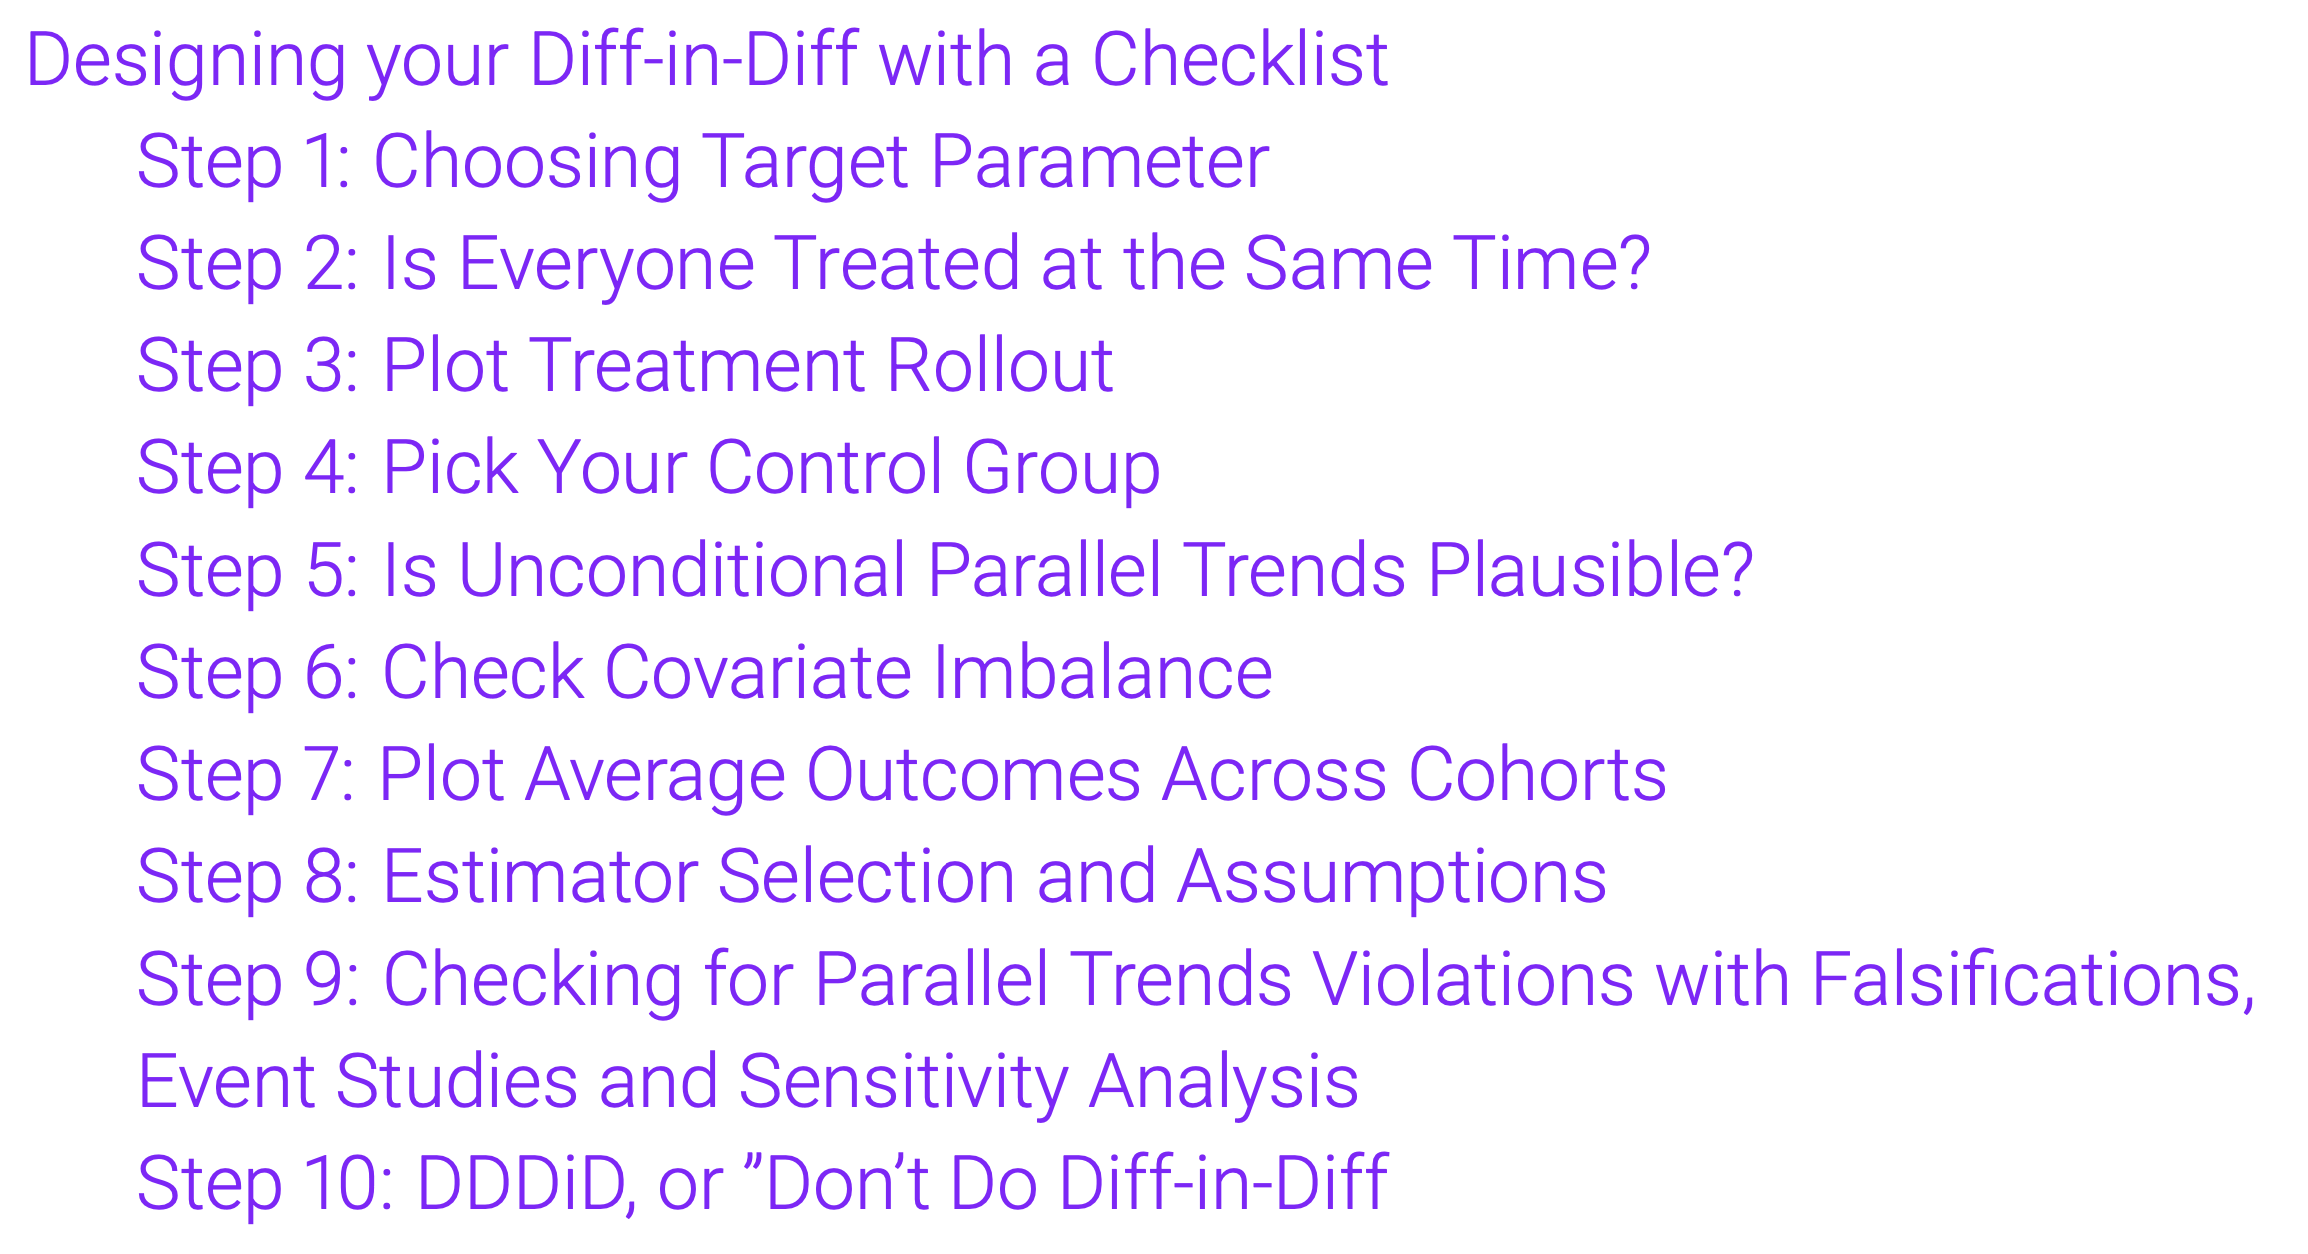
\includegraphics[width=\textwidth]{./lecture_includes/checklist}
\end{figure}

\end{frame}




\begin{frame}{Step 1: Choosing Target Parameter}

\begin{itemize}
\item Lott and Mustard (1997) found that concealed carry gun laws \textbf{reduced murders} using county-level data 1977-1992
\item Subsequent analysis by John Donohue and others would criticize the study on several grounds
	\begin{itemize}
	\item County-level data had problems due to flawed imputation by the FBI
	\item Lack of robustness -- results differed when using state-level data
	\end{itemize}
\item Causal parameters are \emph{averaged treatment effects} and that has two elements
	\begin{itemize}
	\item What population's treatment effects are you averaging
	\item What weight are you using to do that averaging?
	\end{itemize}
\end{itemize}

\end{frame}


\begin{frame}{Average Treatment Effects}

\begin{figure}
    \centering
    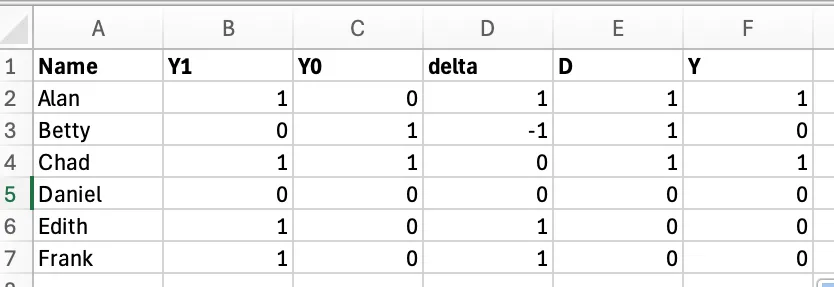
\includegraphics[width=\textwidth]{./lecture_includes/step1_table}
\end{figure}

$ATE =  \frac{1-1+0+0+1+1}{6} = 0.33$

\end{frame}

\begin{frame}{Average Treatment Effects}

\begin{figure}
    \centering
    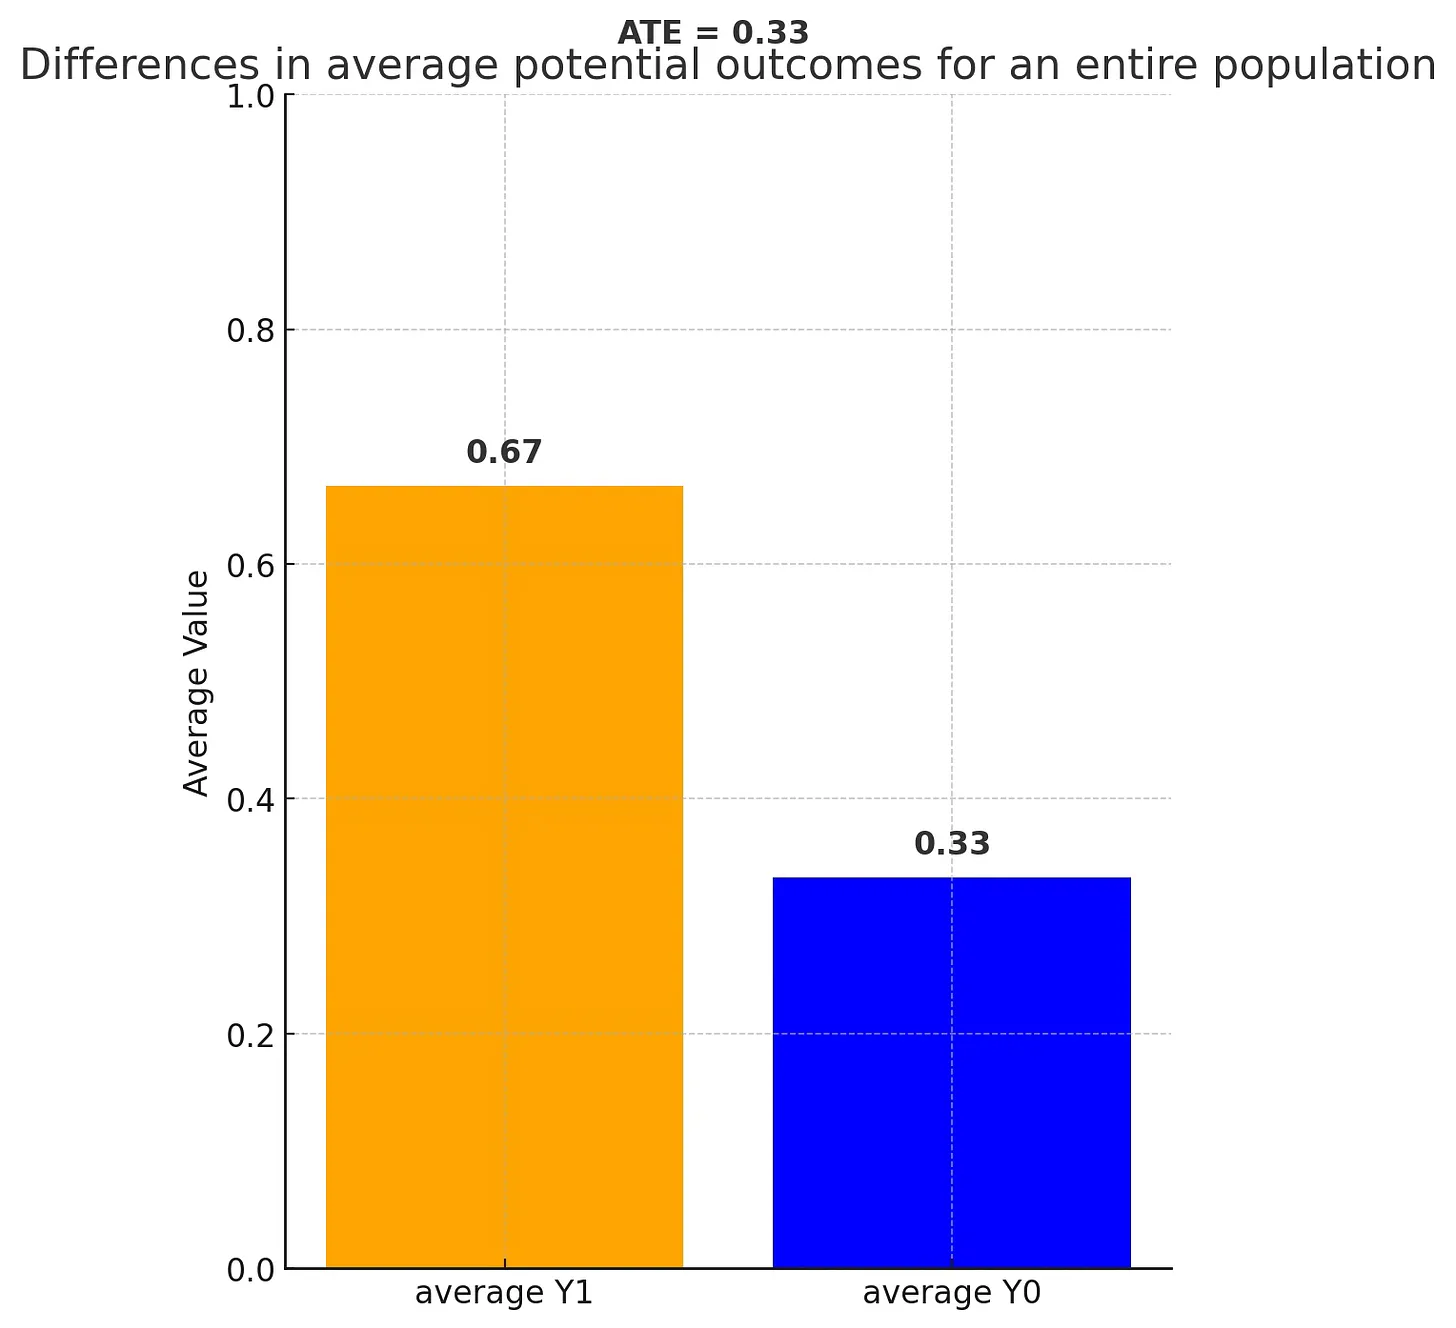
\includegraphics[height=0.8\textheight]{./lecture_includes/step1_y1y0}
\end{figure}


\end{frame}

\begin{frame}{Average Treatment Effect on the Treated}

\begin{figure}
    \centering
    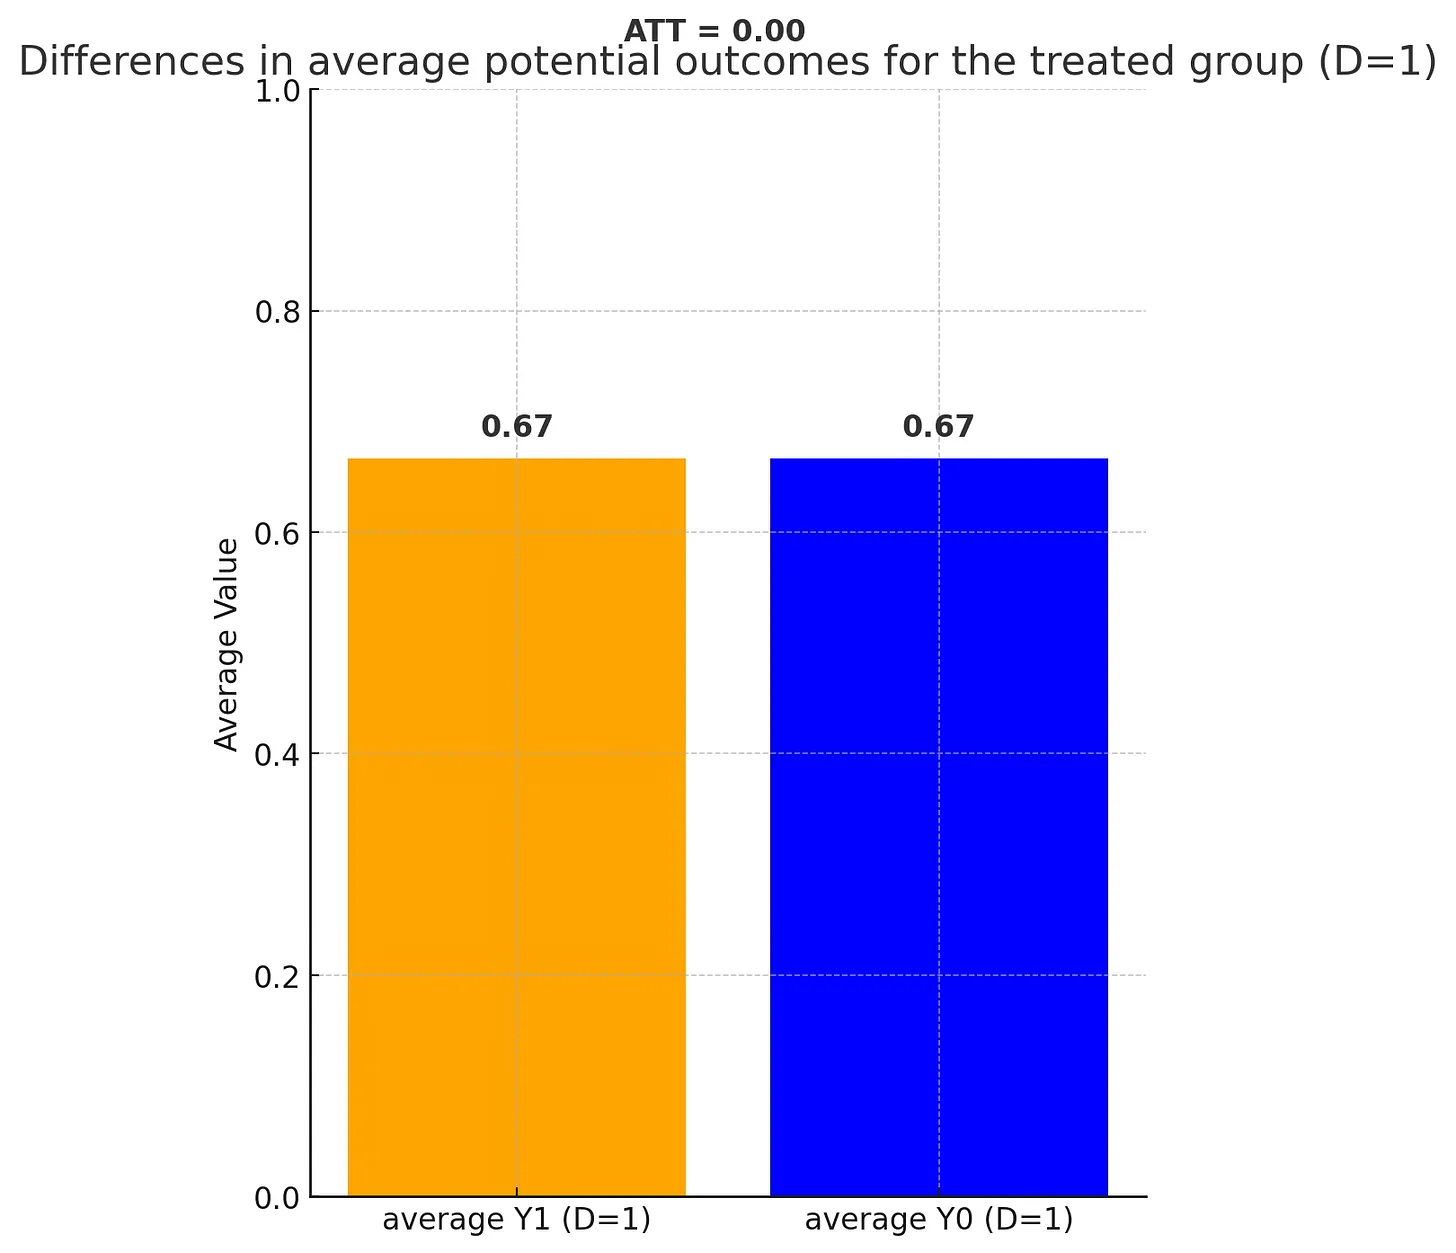
\includegraphics[height=0.8\textheight]{./lecture_includes/step1_att}
\end{figure}


\end{frame}


\begin{frame}{Different Levels of Aggregation, Different Weights}

\begin{figure}
    \centering
    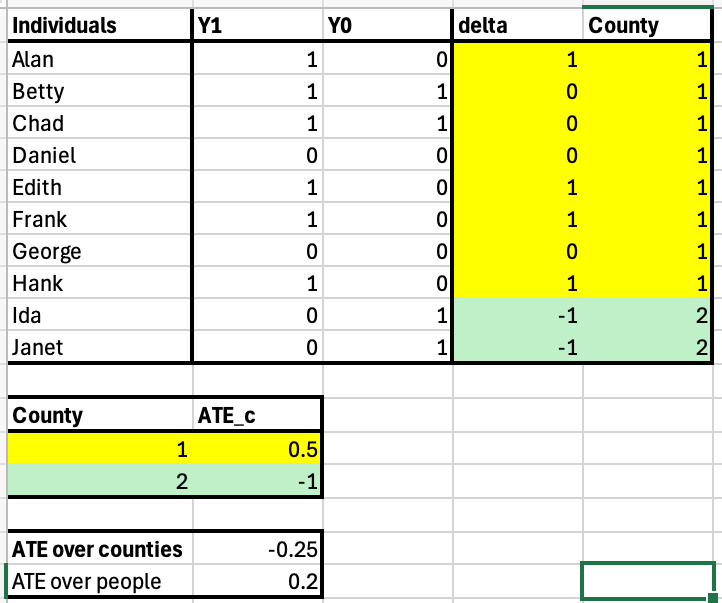
\includegraphics[height=0.8\textheight]{./lecture_includes/step1_weighted}
\end{figure}


\end{frame}

\begin{frame}{Different Levels of Aggregation, Different Weights}


\begin{itemize}
\item Heterogenous treatment effects is causing this, but so is weighting
\item Consider Texas
	\begin{itemize}
	\item Texas has 31 million residents
	\item Texas 254 counties
	\end{itemize}
\item Where do they live?
	\begin{itemize}
	\item 13 million live in Harris, Dallas, Fort Worth, San Antonio and Austin, or rather 41\% 
	\end{itemize}
\item What if concealed carry increases firearm deaths in cities, but reduces them in counties, because of sorting by treatment effects?
\end{itemize}

\end{frame}

\begin{frame}{Simulation}

\begin{itemize}
\item Assume a state with 30 million people and 254 counties
	\begin{itemize}
	\item 15 million live in 5 counties
	\item 15 million live equally spread in the other 249 counties (around 60,000 each)
	\end{itemize}
\item Assume that $\delta_i$ varies, sometimes positive and sometimes negative and $E[Y^1 - Y^0] = 2$
\end{itemize}

\end{frame}

\begin{frame}{Selection into Counties is Random}

\begin{itemize}
\item People choose where to live in Texas, but the mechanism by which they do so will have implications for our datasets
\item What if they sort into counties (i.e., where they live) by lottery
\item Every county will therefore have the same distribution of $Y^1$ and $Y^0$
\item Every county will have an ATE of $2$
\end{itemize}

\end{frame}



\begin{frame}{Average County ATE and Overall ATE Are the Same }

\begin{figure}
    \centering
    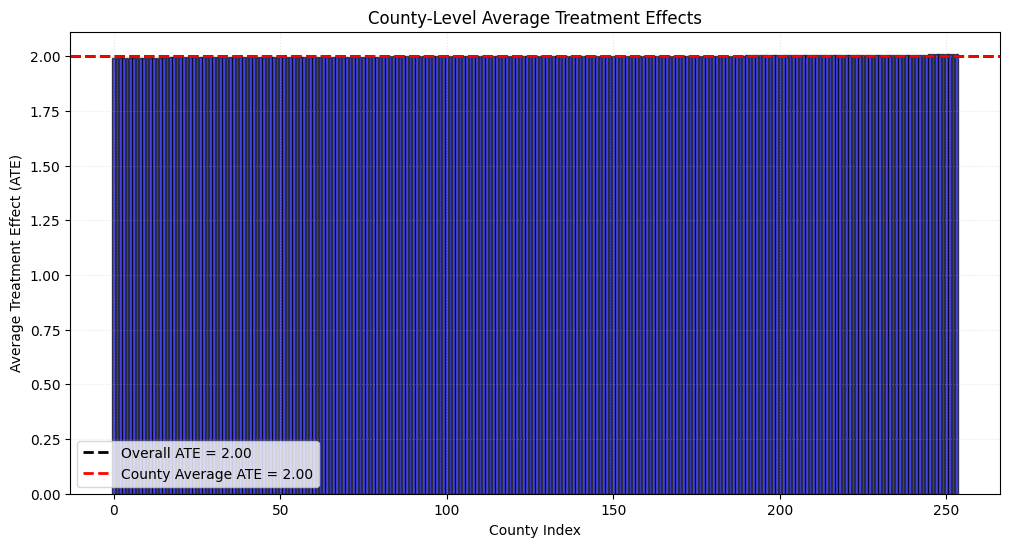
\includegraphics[height=0.7\textheight]{./lecture_includes/tiebout_roy1}
\end{figure}

\end{frame}

\begin{frame}{Selection into Counties is Based on Potential Outcomes}

\begin{itemize}
\item Now assume that people sort into five largest counties have the highest treatment effects ($\delta_i$)
\item Thus the five largest counties are those people for whom concealed carry guns law cause homicides
\item Remaining 249 small counties, in decreasing order, get residents with lower treatment effects (i.e., for whom concealed carry reduces murders)
\end{itemize}

\end{frame}

\begin{frame}{Average County ATE and Overall ATE Differ }

\begin{figure}
    \centering
    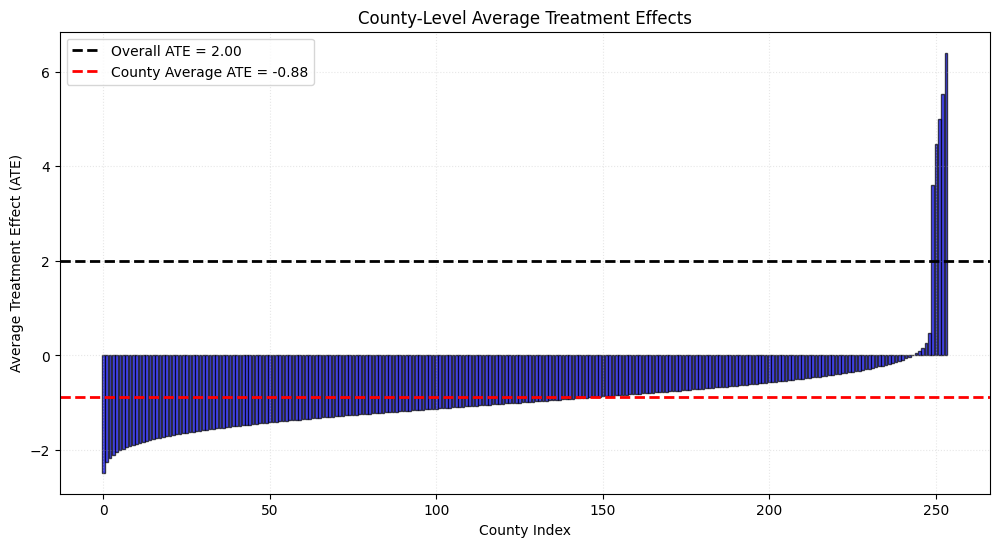
\includegraphics[height=0.7\textheight]{./lecture_includes/tiebout_roy2}
\end{figure}

\end{frame}







\begin{frame}{Both Are Valid, But Not Necessarily Your Research Question}

\begin{itemize}
\item This has implications for what to learn from your dataset which is likely to be aggregated at some level (e.g., individual, city, county, state, country)
\item Do you want to know the ATT for the \emph{average person} or the \emph{average county}?
	\begin{itemize}
	\item It depends on what your study is about
	\item If it about the average person, then you want the overall ATT (i.e., the first case)
	\item If it is about the average county, then you want the county average ATT (i.e., the second case)
	\end{itemize}
\item Since you're averaging over \emph{units} in \emph{data}, it's imperative you make a decision early on as it changes what you decide
\item You can always use population weights but in causal inference, you ask what your target parameter is, and then decide your weights
\end{itemize}

\end{frame}

\subsection{Data Requirements}

\begin{frame}{Longitudinal Data}

\begin{itemize}

\item Diff-in-diff requires four means -- pre and post for two groups
\item Traditionally, the "pre" is a baseline mean at year just prior to treatment, $t-1$ or $b$ depending on author
	\begin{itemize}
	\item Though sometimes you will see people present any interaction as diff-in-diff I will stick to time
	\item Just remember the interaction regression we presented is calculating four means and three subtractions
	\item Interpreting parallel trends is a bit stranger otherwise
	\end{itemize}
\end{itemize}

\end{frame}

\begin{frame}{Longitudinal Data}

\begin{itemize}

\item Two types of longitudinal data:
    \begin{itemize}
      \item Panel Data: same units tracked over time (e.g., National Longitudinal Survey of Youth 1997)
      \item Repeated Cross-Sections: different units sampled at each time (e.g., Census, Current Population Survey)
    \end{itemize}
    \item Violations of parallel trends can arise differently across data types.
\end{itemize}

\end{frame}


% Slide 2
\begin{frame}{What is an Imbalanced Panel?}
  \begin{itemize}
    \item Balanced panel is when all units observed in every period.
    \item Imbalanced panel is when units missing in some periods.
		\begin{itemize}
		\item Anthony is in waves 1-3, 
		\item Bob is in waves 1-3, 
		\item Inez is in waves 1 and 3 only, 
		\item Dignan is in waves 1 and 2 only
		\end{itemize}
    \item Missingness alone does not violate parallel trends, though it does change the parameter.
  \end{itemize}
\end{frame}

\begin{frame}{Example of Balanced ATE}
  \centering
  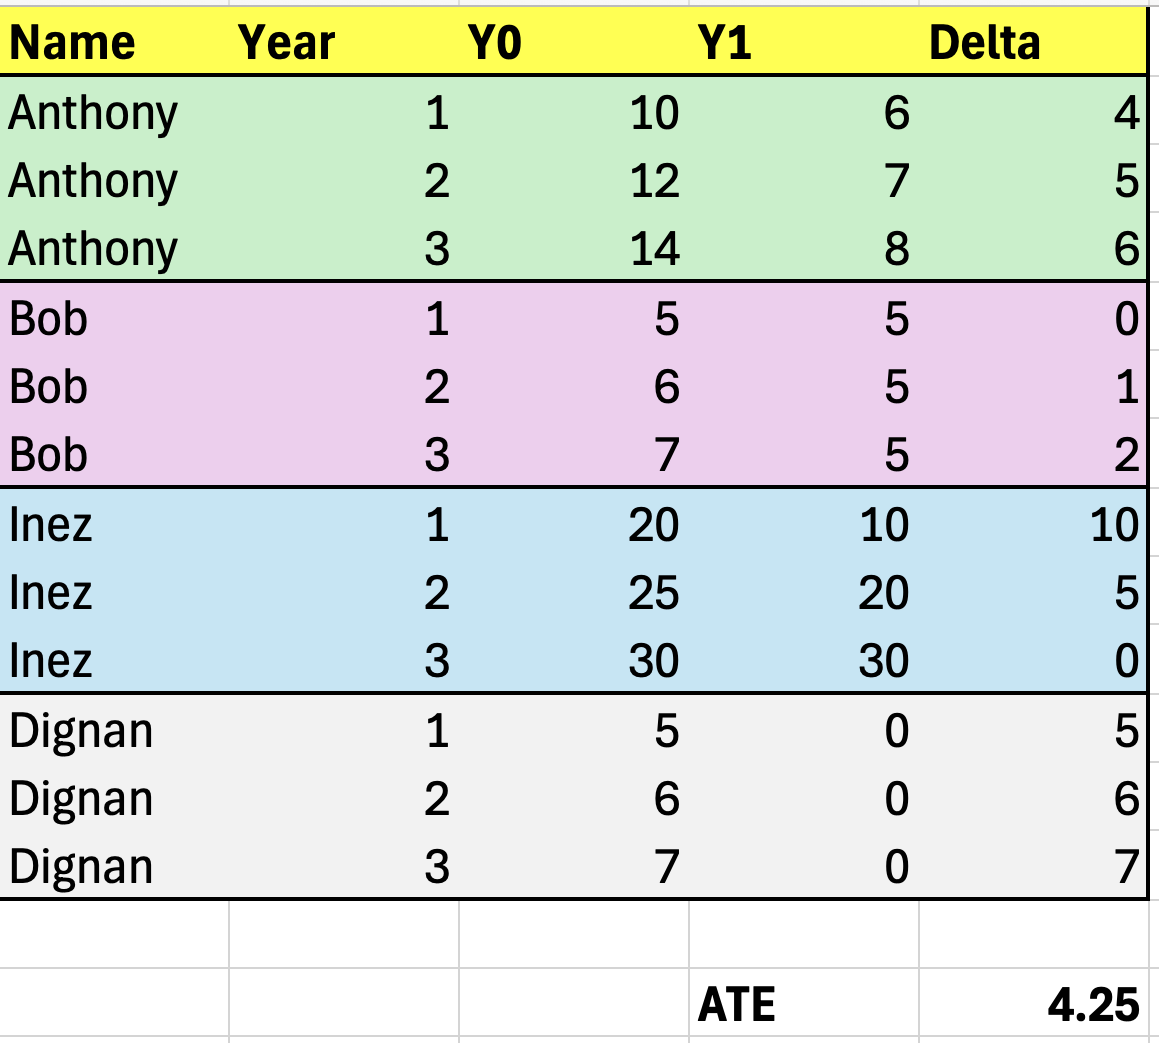
\includegraphics[height=0.85\textheight,keepaspectratio]{./lecture_includes/balanced.png}
\end{frame}


\begin{frame}{How does it change the parameter?}

\begin{itemize}
\item Remember -- in the potential outcomes framework, a treatment effect is defined at the individual level, $\delta_{it}$
\item So if you are missing a person, $i$,  in a period, $t$, then it does not contribute
\item The more heterogeneity in the treatment effects, the more the broken panel will shift away from what you think you're after
\end{itemize}

\end{frame}


\begin{frame}{Imbalanced ATE}
  \centering
  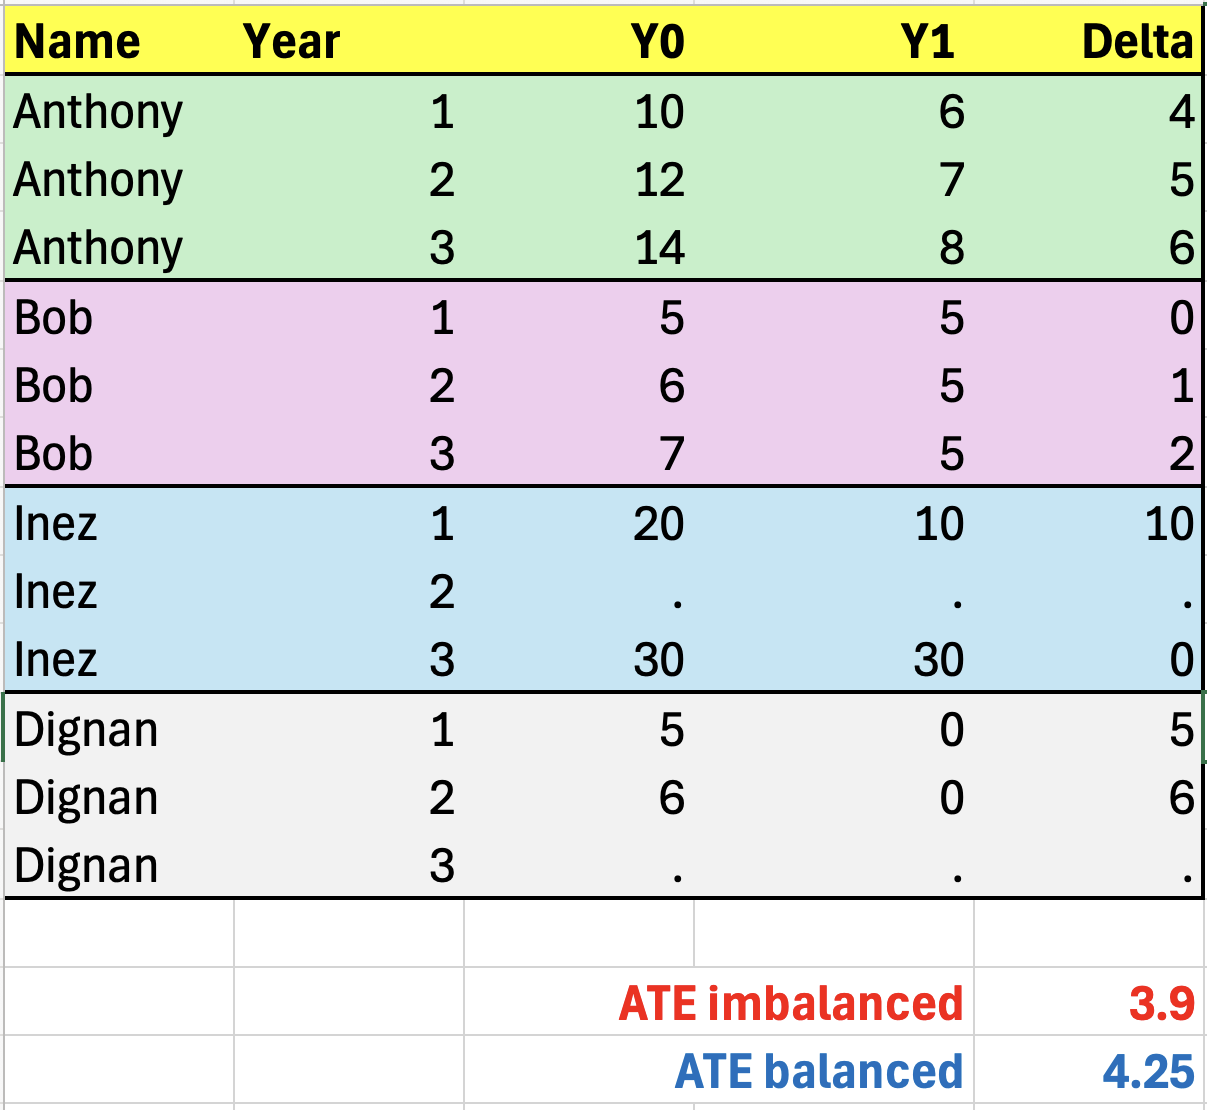
\includegraphics[height=0.85\textheight,keepaspectratio]{./lecture_includes/imbalanced.png}
\end{frame}

% Slide 3
\begin{frame}{Missing at Random (MAR)}
  \begin{itemize}
    \item \textbf{Wooldridge (2010):} MAR does not bias estimation under constant treatment effects.
    \item If missingness is independent of $E[\Delta Y^0]$, then parallel trends will still hold in the large sample.
    \item Wooldridge calls this \emph{Missing At Random (MAR)}
  \end{itemize}
\end{frame}

% Slide 4
\begin{frame}{Non-Random Missingness and Bias}
  \begin{itemize}
    \item But, if the missingness is related to unobservables, then parallel trends may fail.
    \item Example: Small counties with falling murder rates disappear from dataset 
    \item Such selection could bias treatment effects.
  \end{itemize}
\end{frame}

% Slide 5
\begin{frame}{Conditional Missing at Random}
  \begin{itemize}
	\item Might still be salvageable, though there is no prior theory on this and so this is a suggestion for the enterprising student
	\item What if the missing is conditionally random $$Y^0 \perp M \mid X$$
    \item This implies:
    \[ \Pr(M_i = 1 | X_i, Y_i^0, Y_i^1) = \Pr(M_i = 1 | X_i) \]
  \end{itemize}
\end{frame}

\begin{frame}{Conditional Missing at Random}

\begin{itemize}
    \item Missingness depends only on observables
    \item Use methods like Heckman correction or propensity scores
    \item You might explore whether there is something here for you, as it was an idea I had but I haven't worked it out
\end{itemize}

\end{frame}

% Slide 0: Introduction and Value
\begin{frame}
\frametitle{Introduction and Value}
\begin{itemize}
  \item Chained Difference-in-Differences (DiD) (Bellego, Benatia and Dortet-Bernadet 2025) aggregates short-term treatment effects to recover long-term impacts.
  \item It is valuable when balanced panel data is unavailable.
  \item It can be applied to rotating panels (e.g., CPS) as well as imbalanced panels with missing data, making efficient use of overlapping observations.
\end{itemize}
\end{frame}

% Slide 1: Long Difference DID
\begin{frame}
\frametitle{Long Difference DID}
\begin{itemize}
  \item Chained diff-in-diff compares the change in outcomes from a baseline period to a later period for both treated and control groups.
  \item It is defined as: 
    \[
      \text{ATT}(t) = E[Y_t(1) - Y_1(0) \mid \text{D=1}] - E[Y_t(0) - Y_1(0) \mid \text{D=0}]
    \]
  \item This “long difference” cancels out time-invariant characteristics and common trends.
\end{itemize}
\end{frame}

% Slide 2: Overlapping Units
\begin{frame}
\frametitle{Overlapping Units}
\begin{itemize}
  \item Overlap refers to units that are observed in consecutive periods, a common feature in rotating panels.
  \item It is indicated when the sampling indicator satisfies: 
    \[
      S_t \times S_{t+1} = 1
    \]
  \item Such overlap enables the estimation of short-term effects even without a fully balanced panel.
\end{itemize}
\end{frame}

% Slide 3: Exact Calculation (2×2 Formula)
\begin{frame}
\frametitle{Exact Calculation (2×2 Formula)}
\begin{itemize}
  \item For each pair of consecutive periods, the short-term DiD effect is computed as:
    \[
      \text{DiD}_t = E(Y_{t+1} - Y_t \mid \text{treated}) - E(Y_{t+1} - Y_t \mid \text{control})
    \]
  \item The long-term effect is obtained by summing these differences:
    \[
      \text{Long DiD} = \sum_{t=1}^{T-1} \text{DiD}_t
    \]
  \item This formula is consistent with the potential outcomes framework.
\end{itemize}
\end{frame}

% Slide 4: Final Target Parameter
\begin{frame}
\frametitle{Final Target Parameter}
\begin{itemize}
  \item The target parameter is the long-run average treatment effect on the treated (ATT).
  \item It is expressed as:
    \[
      \text{ATT}(t) = E[Y_t(1) - Y_t(0) \mid \text{treated}]
    \]
  \item This represents the cumulative impact of the treatment over time.
\end{itemize}
\end{frame}

% Slide 5: Building Blocks
\begin{frame}
\frametitle{Building Blocks}
\begin{itemize}
  \item The method builds on estimating one-period DID effects between consecutive time periods.
  \item Each building block is given by:
    \[
      \Delta \text{ATT}(\tau) = E(Y_{\tau+1} - Y_\tau \mid \text{treated}) - E(Y_{\tau+1} - Y_\tau \mid \text{control})
    \]
  \item These “chain links” are summed to recover the overall long-term effect.
\end{itemize}
\end{frame}

% Slide 6: Weights
\begin{frame}
\frametitle{Weights and Sampling Indicators}
\begin{itemize}
  \item Recall from earlier \(S_{i,t}\) is an indicator that equals 1 if unit \(i\) is observed in period \(t\) (and 0 otherwise).
  \item Define the overlap indicator as \(S_{i,\tau,\tau+1} = S_{i,\tau} \times S_{i,\tau+1}\), which is 1 if unit \(i\) is observed in both period \(\tau\) and \(\tau+1\).
  \item The weight for unit \(i\) for the period pair \(\tau,\tau+1\) is:
    \[
      w_{i,\tau} = \frac{S_{i,\tau,\tau+1}}{\sum_{j} S_{j,\tau,\tau+1}},
    \]
    ensuring that each short-term DID effect is appropriately scaled based on the number of overlapping observations.
\end{itemize}
\end{frame}

% Slide 7: Standard Error Calculation
\begin{frame}
\frametitle{Standard Error Calculation}
\begin{itemize}
  \item Standard errors are computed by aggregating the variances of the individual short-term DID estimates.
  \item Analytical derivations use influence functions or a generalized method of moments (GMM) approach to combine errors from each link.
  \item Bootstrapping methods (e.g., multiplier bootstrap) are often used to account for clustering and the overlap structure, ensuring robust inference.
\end{itemize}
\end{frame}

\begin{frame}{Code}

\begin{itemize}
\item R package is available at CRAN as \texttt{cdid}
\item Documentation: \url{https://cran.r-project.org/web/packages/cdid/cdid.pdf}
\item Github: \url{https://github.com/joelcuerrier/cdid}
\end{itemize}

\end{frame}


\begin{frame}{Repeated cross-sections and compositional change}
	
	\begin{itemize}
	\item One of the risks of a repeated cross-section is that the composition of the sample may have changed between the pre and post period in ways that are correlated with treatment
	\item Hong (2013) uses repeated cross-sectional data from the Consumer Expenditure Survey (CEX) containing music expenditure and internet use for a random sample of households
	\item Study exploits the emergence of Napster (first file sharing software widely used by Internet users) in June 1999 as a natural experiment
	\item Study compares internet users and internet non-users before and after emergence of Napster
	\end{itemize}

\end{frame}

\begin{frame}{Introduction of Napster and spending on music}
	\begin{figure}
	\includegraphics[scale=0.5]{./lecture_includes/hong_napster}
	\end{figure}
	
\end{frame}


\begin{frame}[plain]
	\begin{figure}
	\includegraphics{./lecture_includes/Hong_1.pdf}
	\end{figure}
	
\end{frame}



\begin{frame}{Repeated Cross Section Risks}

\begin{itemize}
\item Repeated cross sections have their own challenges that panels don't in that the group could be shifting compositionally
\item Detect using a balance table with covariates highly predictive of the missing $E[Y^0|D=1]$ for this exercise 
	\begin{itemize}
	\item Percent of cat owners is probably irrelevant to trends in potential outcomes
	\item But age and income is probably relevant for spending habits
	\item We'll discuss covariates more later, but for now just consider what characteristics are relevant to your outcome
	\end{itemize}
\item Documenting covariates that are cannot be affected by the treatment like this table is a way to check for \emph{compositional changes} in the sample
\end{itemize}

\end{frame}


\begin{frame}{Changes Between Internet and Non-Internet Users Over Time}
  \tiny
  \centering
  \begin{table}[htb]
    \caption{Changes Between Internet and Non-Internet Users Over Time}
    \begin{tabular}{lcccccc}
      \toprule
      \textbf{Characteristic} &
         \multicolumn{2}{c}{\textbf{1997}} &
         \multicolumn{2}{c}{\textbf{1998}} &
         \multicolumn{2}{c}{\textbf{1999}} \\
         & \textbf{User} & \textbf{Non-user} &
           \textbf{User} & \textbf{Non-user} &
           \textbf{User} & \textbf{Non-user} \\
      \midrule
      \emph{Demographics} \\
      Age & 40.2 & 49.0 & 42.3 & 49.0 & 44.1 & 49.4 \\
      Income & \$52,887 & \$30,459 & \$51,995 & \$26,189 & \$49,970 & \$26,649 \\
      High school graduate & 0.18 & 0.31 & 0.17 & 0.32 & 0.21 & 0.32 \\
      Some college & 0.37 & 0.28 & 0.35 & 0.27 & 0.34 & 0.27 \\
      College grad & 0.43 & 0.21 & 0.45 & 0.21 & 0.42 & 0.20 \\
      Manager & 0.16 & 0.08 & 0.16 & 0.08 & 0.14 & 0.08 \\
      \bottomrule
    \end{tabular}
  \end{table}
  

\end{frame}



\begin{frame}{What was this table about?}

\begin{itemize}
\item  Notice that users are getting older and poorer -- both of which predict spending less money on music
\item If these covariates are themselves predictive of trends, then it is suggestive parallel trends could be \emph{mechanically} breaking, so check $$X_{it} = \alpha + \beta_1 D_i + \beta_t Post_t + \delta ( D_i \times Post_t ) + \varepsilon_{it}$$ 
\item Or consider the normalized difference in means table we discuss later
\item If violated, then consider the following fix by Hong (2013) which adjusts for propensity scores in both periods
\end{itemize}

\end{frame}



\begin{frame}{Step 1. Estimate Propensity Scores}
\begin{itemize}
  \item Estimate two separate propensity scores for the treatment group based on observed characteristics:
  \item Pre-treatment period ($T = 0$):
  \begin{equation*}
    P_b = \Pr(D=1 \mid T=0, X)
  \end{equation*}
  \item Post-treatment period ($T = 1$):
  \begin{equation*}
    P_a = \Pr(D=1 \mid T=1, X)
  \end{equation*}
  \item Time-specific scores allow for balancing in each period.
\end{itemize}
\end{frame}

\begin{frame}{Step 2. Weight Observations Using Propensity Scores}
\begin{itemize}
  \item Use inverse probability weighting (IPW) to balance samples:
  \item Pre-treatment ($T = 0$):
  \begin{equation*}
    E_w[Y \mid D = 1, T = 0] = \frac{\sum_{i} w_{i} Y_{i}}{\sum_{i} w_{i}}, \quad w_{i} = \frac{1}{P_b}
  \end{equation*}
  \begin{equation*}
    E_w[Y \mid D = 0, T = 0] = \frac{\sum_{i} (1 - w_{i}) Y_{i}}{\sum_{i} (1 - w_{i})}, \quad w_{i} = \frac{1}{1 - P_b}
  \end{equation*}
  \item Post-treatment ($T = 1$):
  \begin{equation*}
    E_w[Y \mid D = 1, T = 1] = \frac{\sum_{i} w_{i} Y_{i}}{\sum_{i} w_{i}}, \quad w_{i} = \frac{1}{P_a}
  \end{equation*}
  \begin{equation*}
    E_w[Y \mid D = 0, T = 1] = \frac{\sum_{i} (1 - w_{i}) Y_{i}}{\sum_{i} (1 - w_{i})}, \quad w_{i} = \frac{1}{1 - P_a}
  \end{equation*}
\end{itemize}
\end{frame}

\begin{frame}{Step 3. Calculate the Adjusted Difference-in-Differences}
\begin{itemize}
  \item Use the weighted averages to compute the adjusted DiD estimator:
  \begin{align*}
    \text{Adjusted DiD} &= \left( E_w[Y \mid D = 1, T = 1] - E_w[Y \mid D = 0, T = 1] \right) \\
    &\quad - \left( E_w[Y \mid D = 1, T = 0] - E_w[Y \mid D = 0, T = 0] \right)
  \end{align*}
  \item This accounts for compositional change and enhances credibility of ATT estimation in repeated cross-sections.
\end{itemize}
\end{frame}


\begin{frame}{Repeated cross-sections}

\begin{itemize}
\item Surprisingly underappreciated problem with almost no literature around it
\item ``Difference-in-differences with Compositional Changes'' by Pedro Sant'Anna and Qi Xu (2023) is an update to Hong (2013) (in our readings)
\end{itemize}

\end{frame}






\begin{frame}
 
\begin{figure}
    \centering
    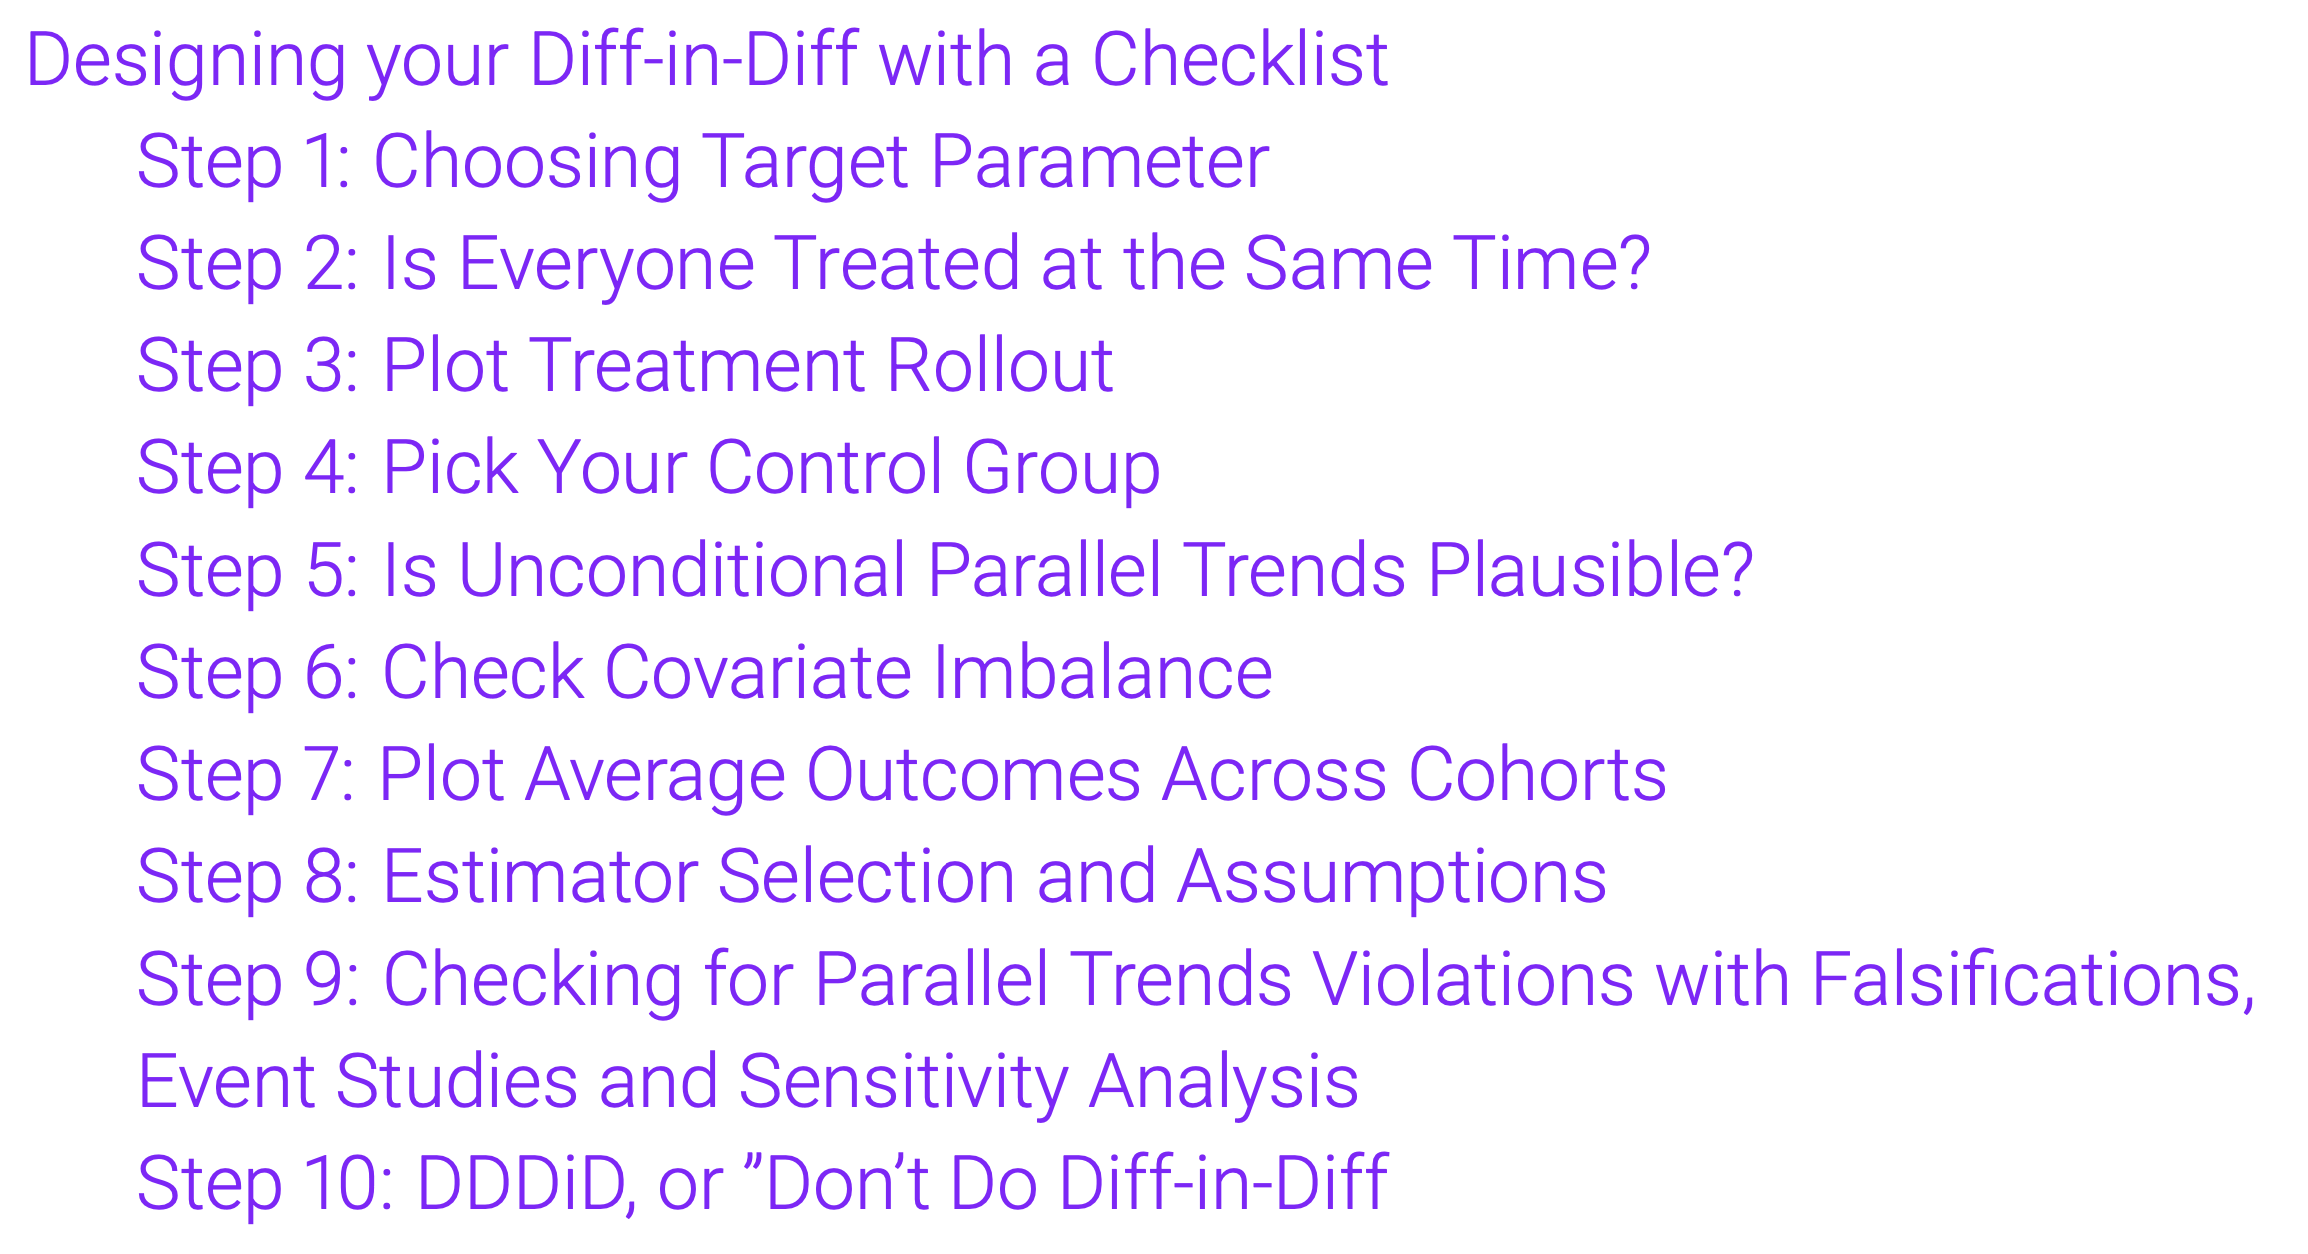
\includegraphics[width=\textwidth]{./lecture_includes/checklist}
\end{figure}

\end{frame}

\begin{frame}{Step 2: Is Everyone Treated at the Same Time?}

\begin{itemize}
\item Cohorts and groups words used interchangeably in diff-in-diff
\item Cohorts describe \emph{when} units were treated at the same time
\item Count those units and show them in a table so that we can see who is in each cohort, how large they are, and when this happened
\item Include the "already treated" and the "never treated" in your counts if they exist
\end{itemize}

\end{frame}

\begin{frame}

\begin{figure}
    \centering
    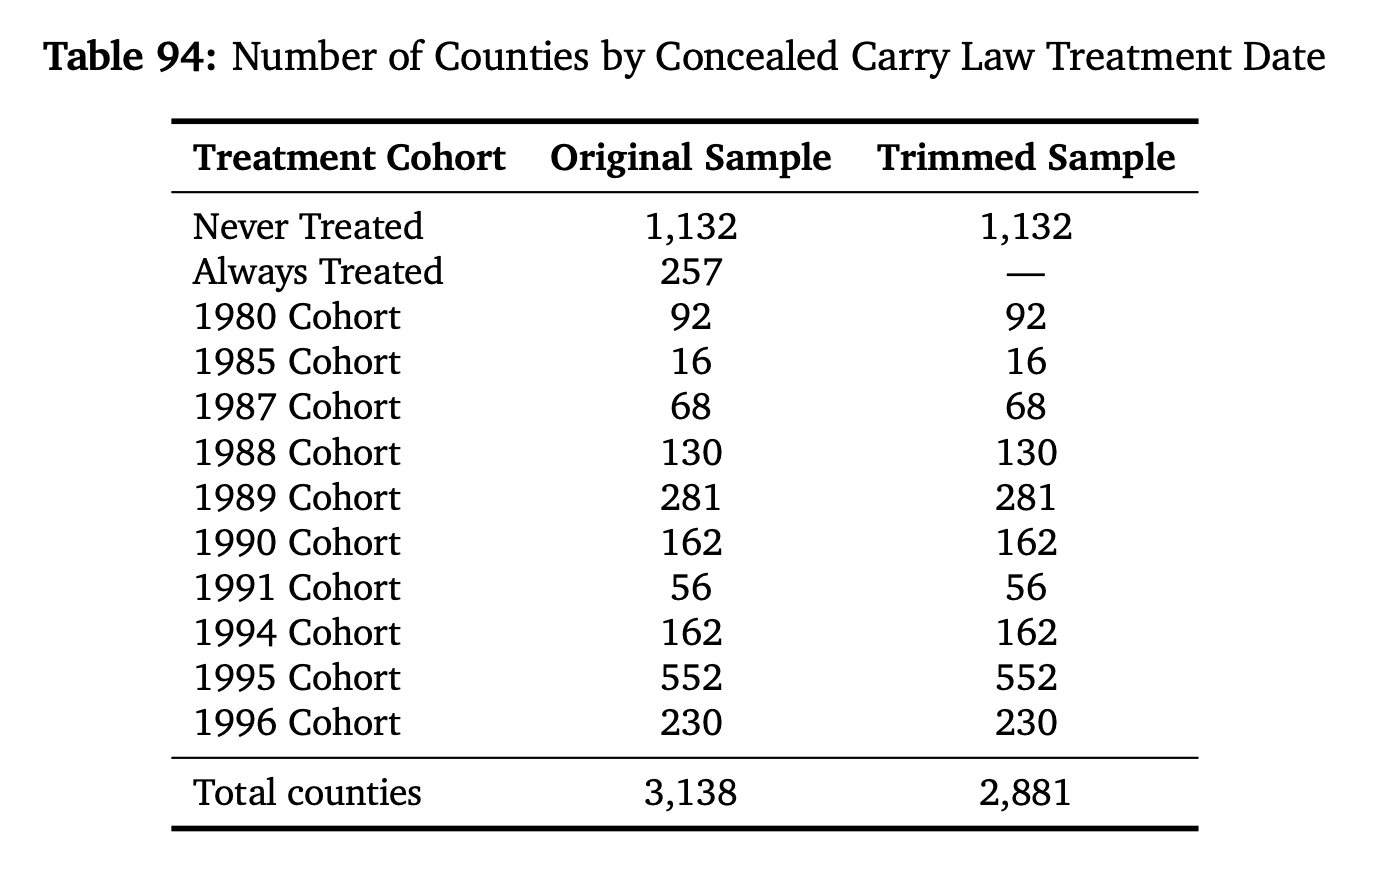
\includegraphics[height=0.8\textheight]{./lecture_includes/treated_at_same_time}
\end{figure}

\end{frame}


\begin{frame}{Why are we doing this?}

\begin{itemize}

\item Slowing down is key to the designing of the process
\item We should be able to say precisely who is and is not in each period, in each group
\item Automating this is best, though, and thankfully ChatGPT can help us automate this process in our code
\item Be sure you count "already treated" because as we will see these are dangerous to have in the sample
\end{itemize}

\end{frame}



\begin{frame}
 
\begin{figure}
    \centering
    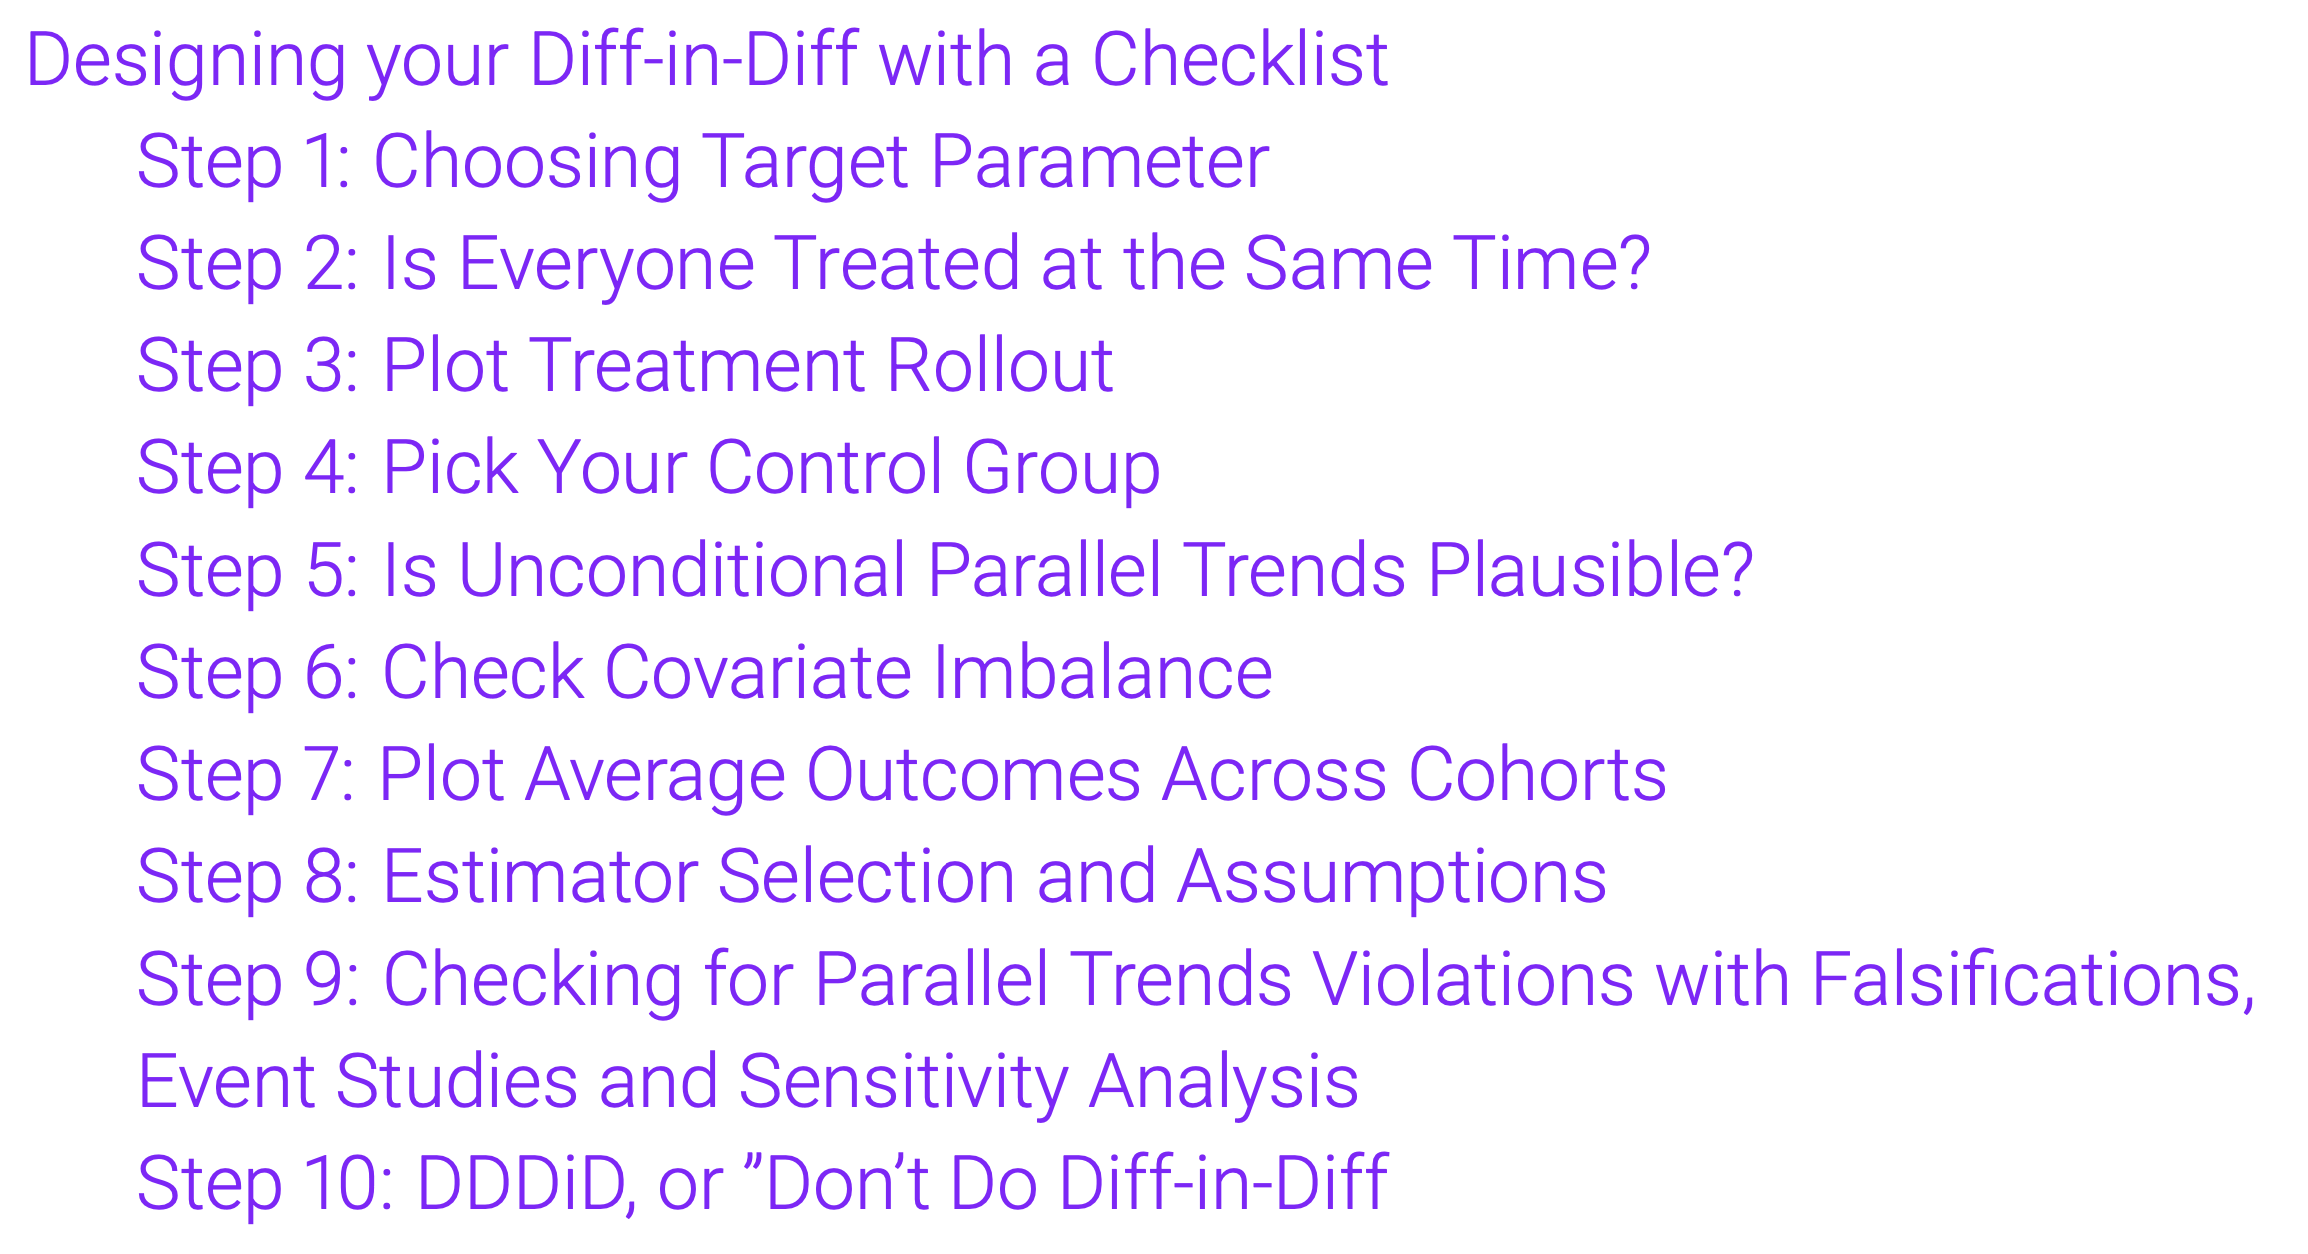
\includegraphics[width=\textwidth]{./lecture_includes/checklist}
\end{figure}

\end{frame}

\begin{frame}{Step 3: Plot the treatment rollout}

\begin{itemize}

\item Step 2 only allowed us to count the size of our cohorts
\item But now we need to see how the treatments spread across time for each group
\item Easy way is to use Yiqing Xu, et al.'s code \texttt{PanelView} available in Stata and R
\item Syntax is very flexible, but I like to show pre, post and never-treated with the outcome specified so I can check the missingness
\end{itemize}

\end{frame}

\begin{frame}{Step 3: Plot Treatment Rollout}

\begin{figure}
    \centering
    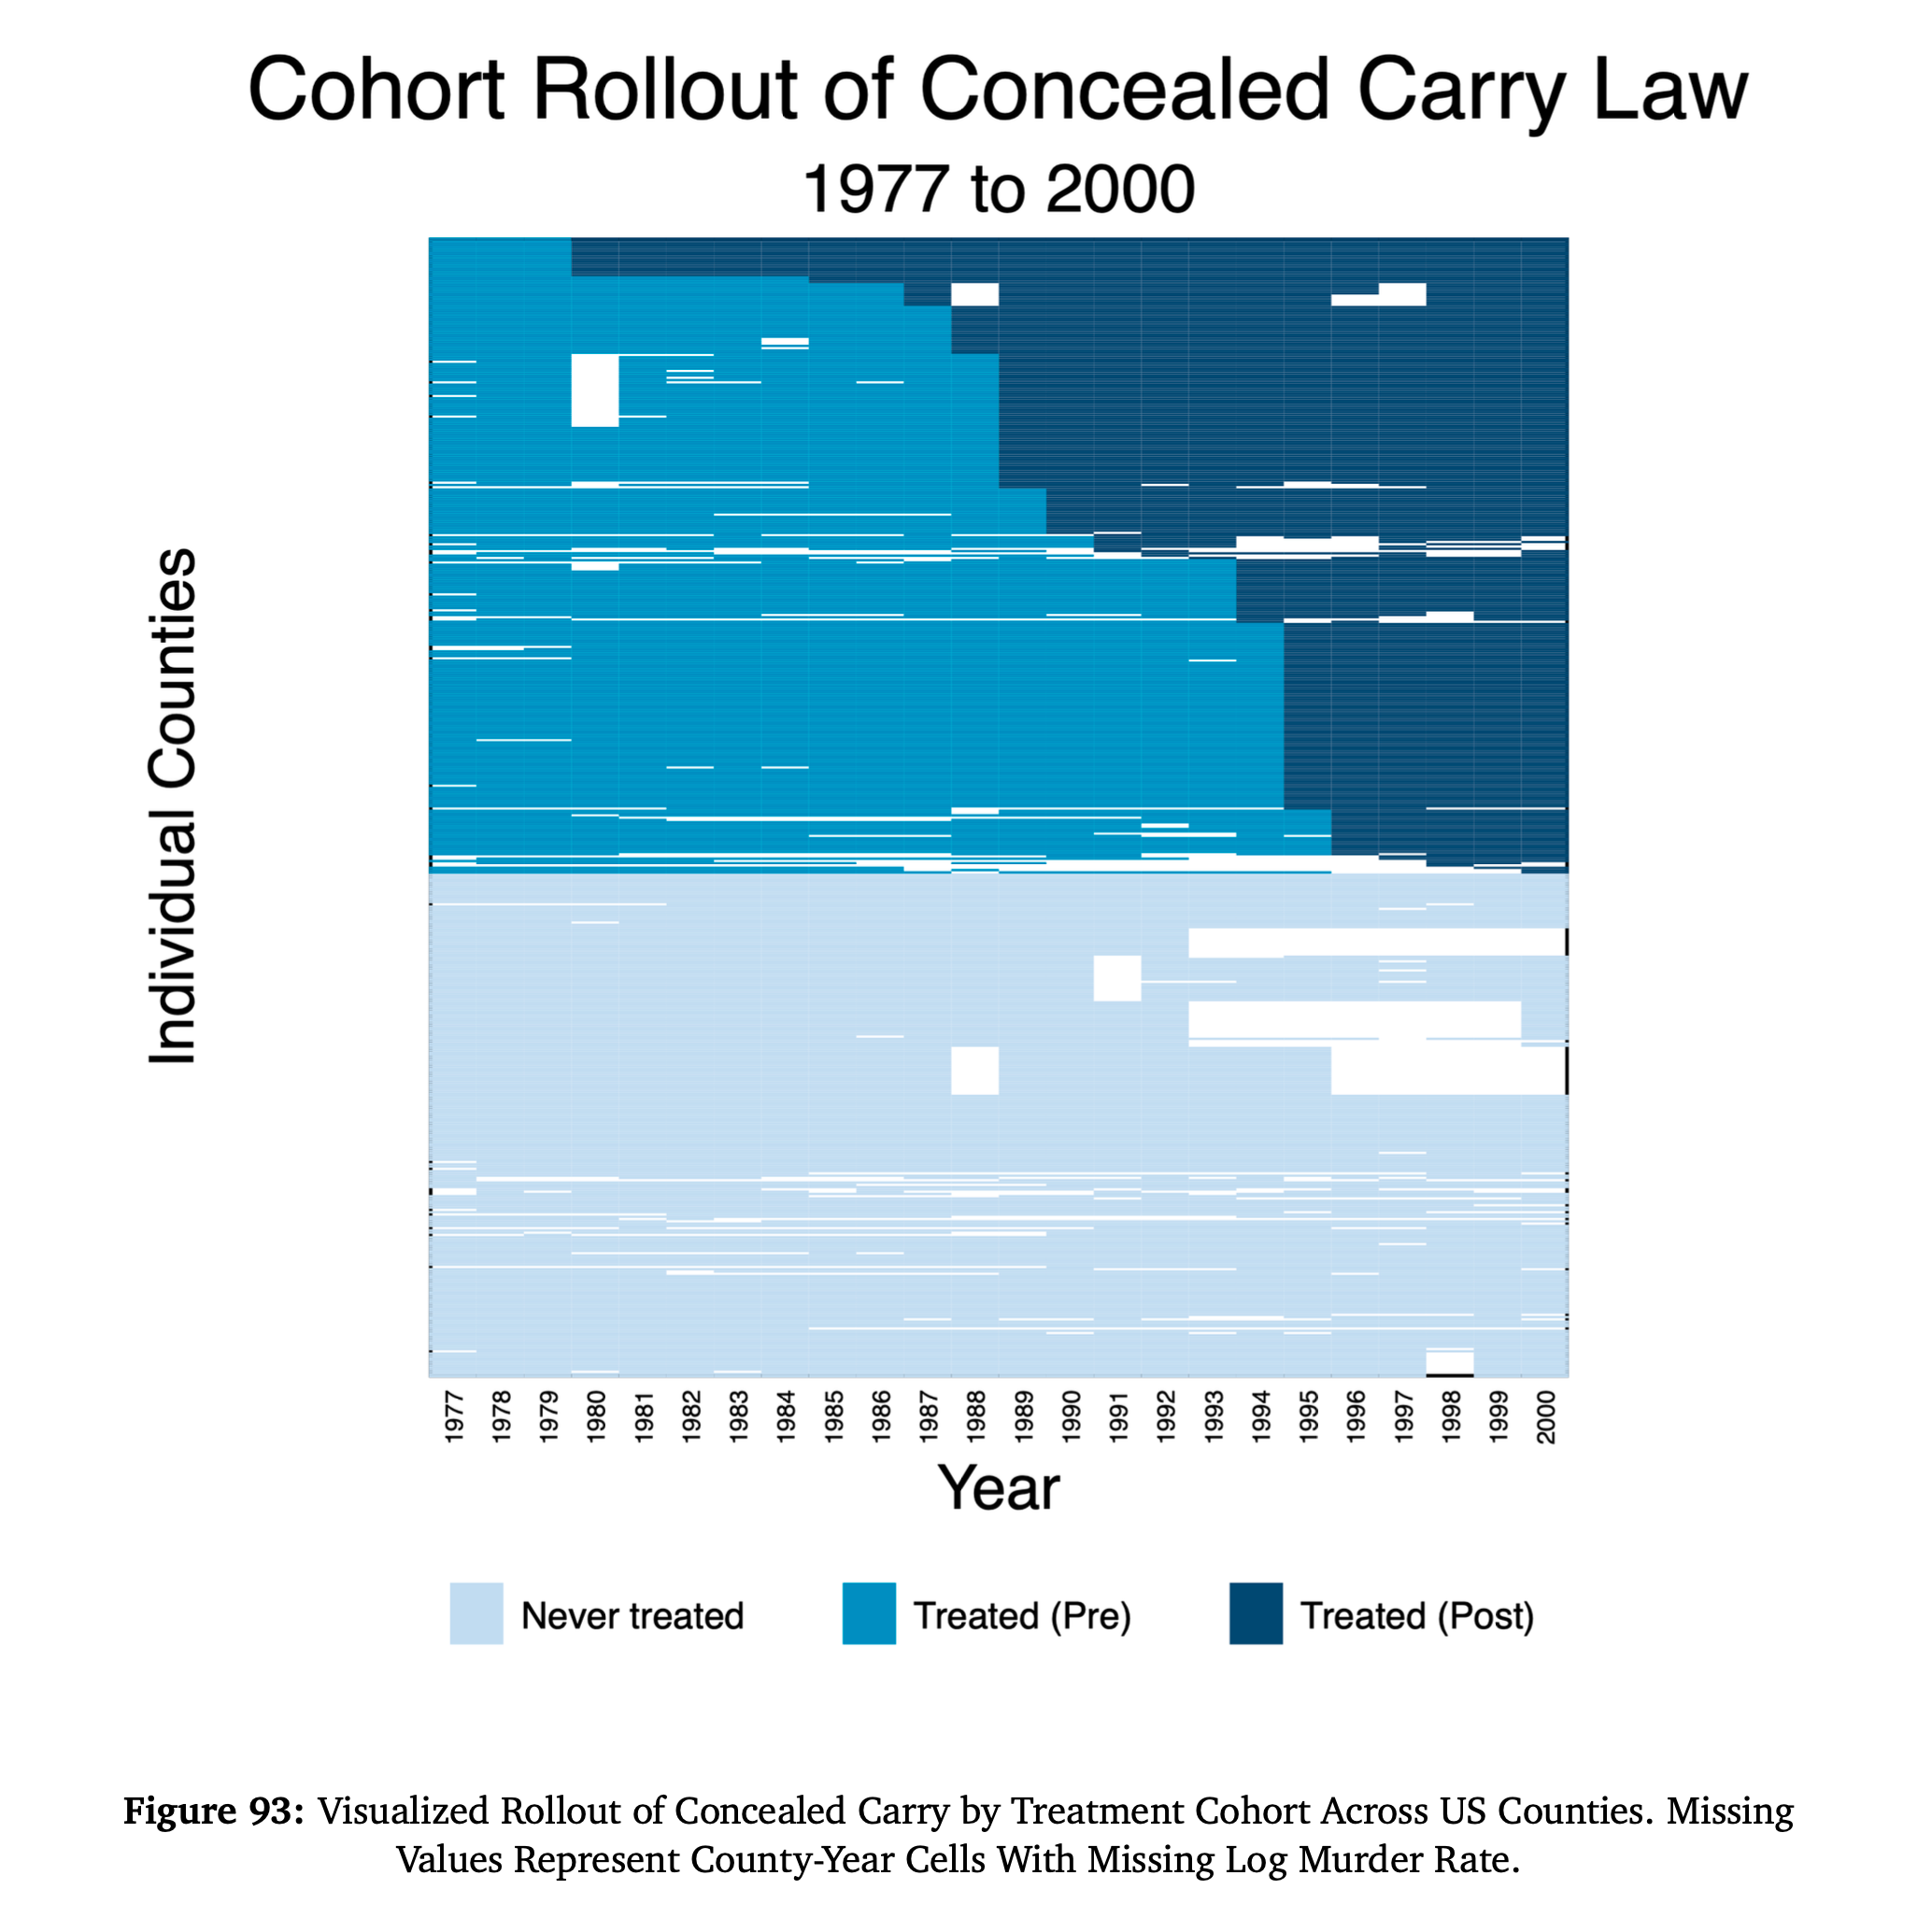
\includegraphics[height=0.95\textheight]{./lecture_includes/step3_panelview}
\end{figure}

\end{frame}


\begin{frame}{Major missingness problems}

\begin{itemize}

\item Could be we will have to dig a bit into these data to salvage it -- this was in fact one of the criticisms of the county level data
\item Could be a candidate for chained diff-in-diff
\item Remember -- if our goal is the county-level target parameter, then simply switching to the state-level crime data would defeat the purpose of the study
\item But now we are realizing what we are up against
\item You \textbf{do not} want to be the last one to realize the problem you have -- God forbid Data Colada figures it out first!

\end{itemize}

\end{frame}

\begin{frame}
 
\begin{figure}
    \centering
    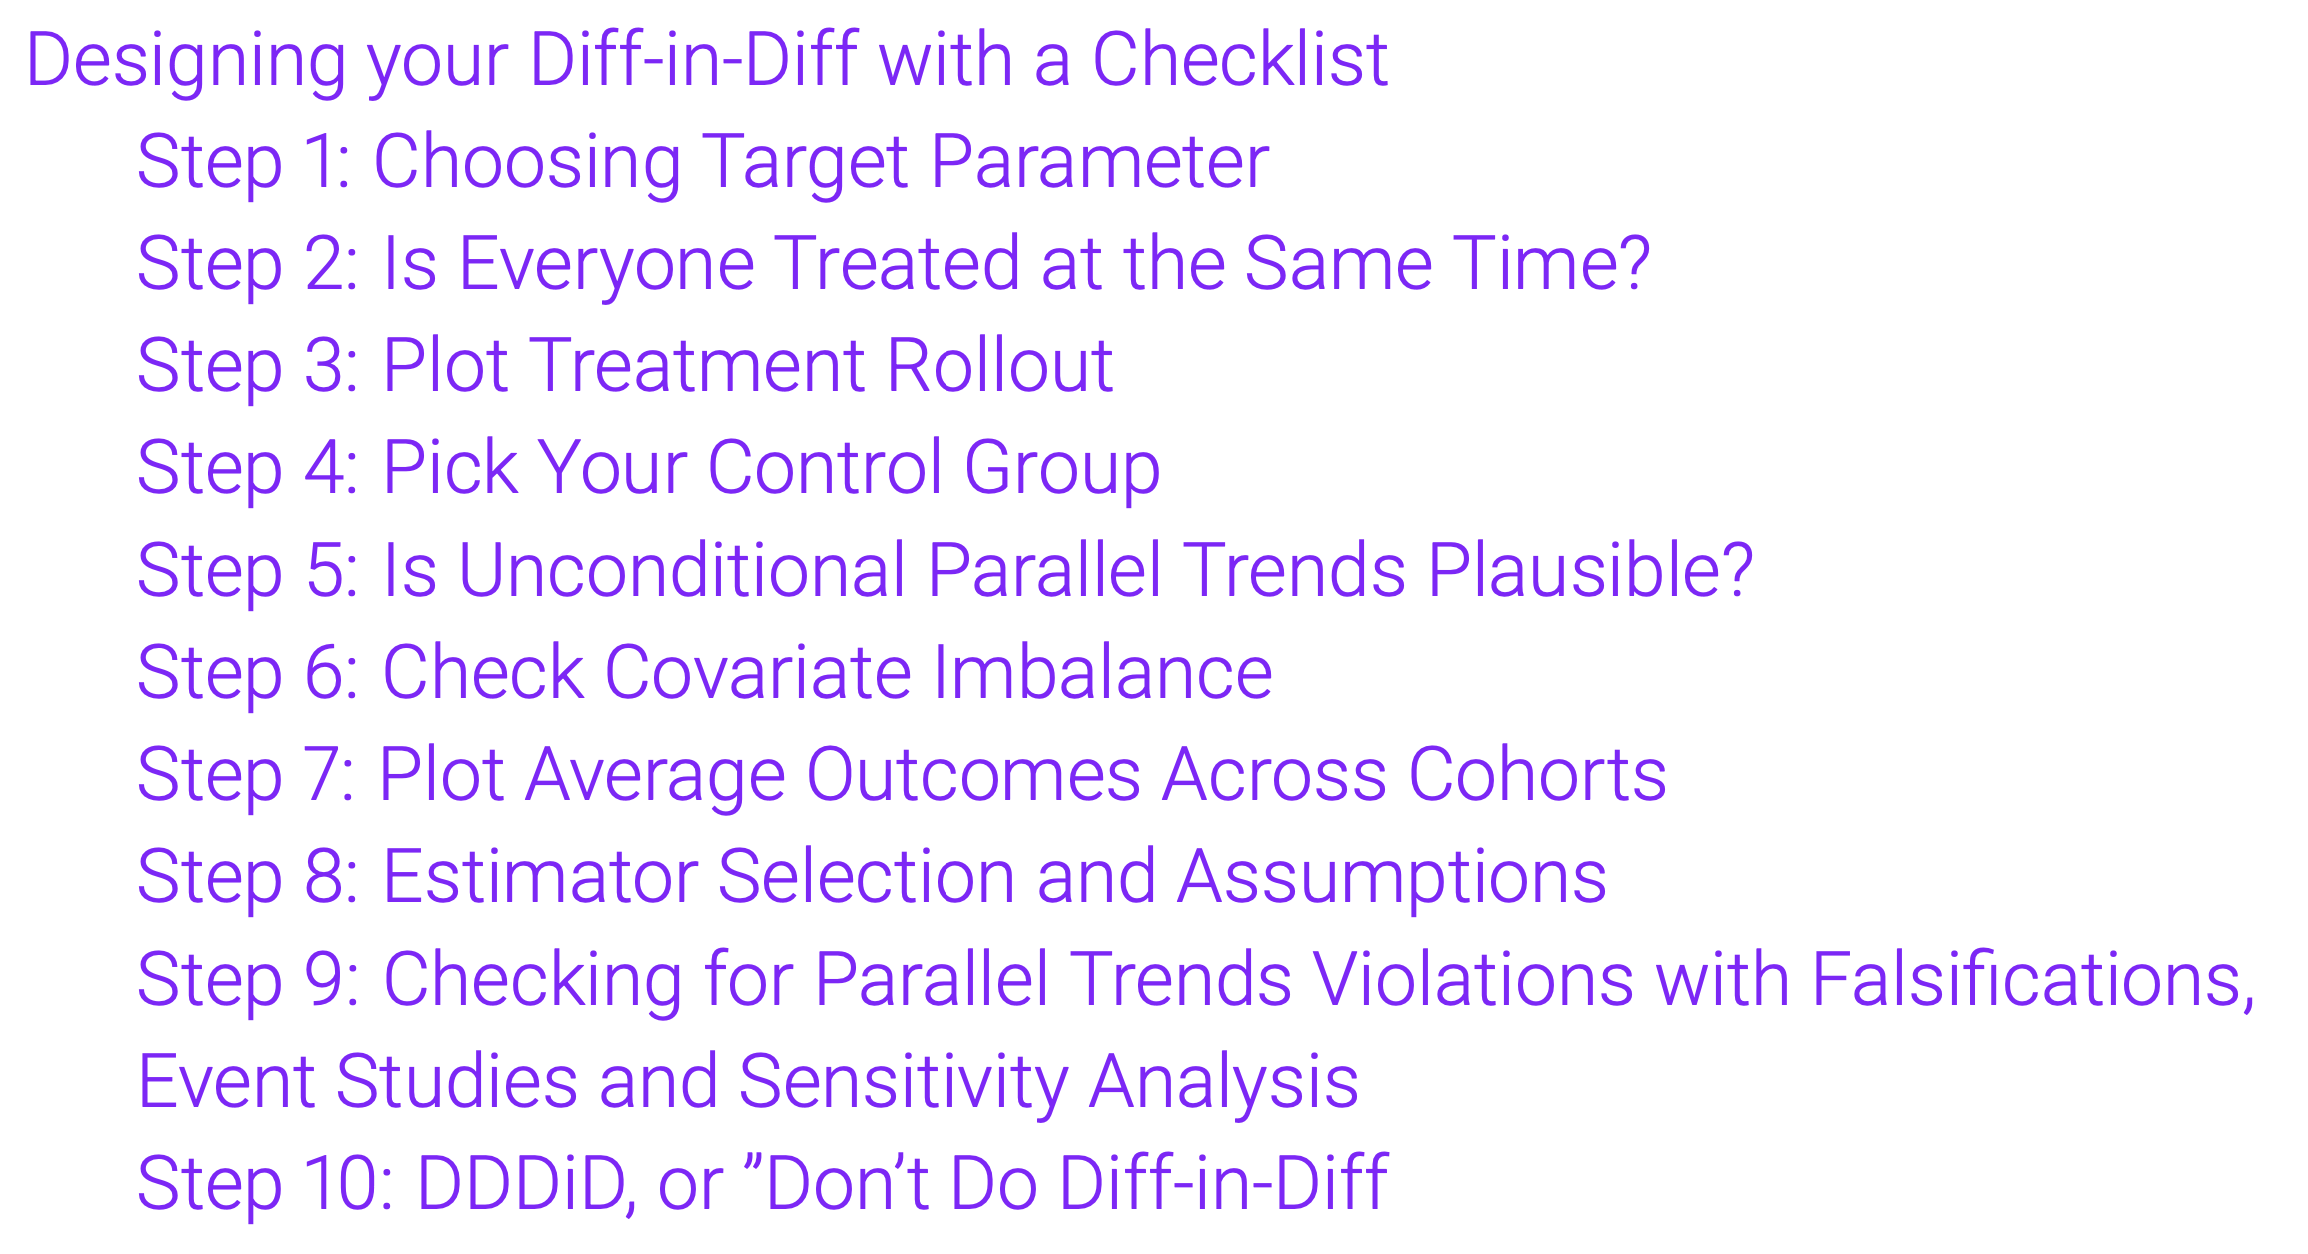
\includegraphics[width=\textwidth]{./lecture_includes/checklist}
\end{figure}

\end{frame}


\begin{frame}{Step 4: Pick Your Control Group}

\begin{itemize}

\item One of the sins created by OLS was the ability to throw the kitchen sink into one model and never know who was being compared to who
	\begin{itemize}
	\item Causal inference is hard and easy -- don't confuse the hard with the easy
	\item If you can't say who the comparison group is, start there because it should be you choosing it, not the model
	\end{itemize}
\item Parallel trends is about whether your control group is a correct proxy for the missing potential outcome for your treatment group, so it's natural to ask who do you want it to be?
\end{itemize}

\end{frame}

\begin{frame}{Step 4: Pick Your Control Group}

\begin{itemize}

\item Do you want to compare treated units with never treated units?
	\begin{itemize}
	\item Weird that they never got treated though right?
	\end{itemize}
\item Or do you want to compare with not-yet-treated?  After all -- didn't they get treated too?
\end{itemize}

\end{frame}

\begin{frame}{Selecting your control group}

\begin{itemize}
\item There's three different control groups you can have in diff-in-diff:
	\begin{enumerate}
	\item \textcolor{red}{Already treated group -- Don't do it}
	\item Never treated group -- maybe do it 
	\item Not-yet-treated group -- maybe do it
	\end{enumerate}
\item Selection is largely shaping which of the second and third ones is more likely to satisfy parallel trends
\item No way to rank it, but we know the more random the assignment, the more likely (2) and (3) are the same thing
\item Share anecdote about driver license law and undocumented workers
\end{itemize}

\end{frame}




\begin{frame}{What does "selection" mean?}

\begin{itemize}
\item Selection is a phrase you hear often but what does it mean?
\item Ex: Some people are in the treatment group and some aren't:
	\begin{enumerate}
	\item \textbf{Who} and \textbf{which} people are treated and aren't is observed and coded with $D$
	\item \textbf{Why} and \textbf{how} is not coded, but matters in causal inference \emph{a lot}
	\end{enumerate}
\item Selection has to do with the "why" and "how" the units were chosen to be treated
\end{itemize}

\end{frame}

\begin{frame}{Two extreme forms of selection}

\begin{itemize}
\item Randomization.  Ten people, 5 treated and 5 aren't, but the assignment happened with coin flips versus
\item Sorting.  The 5 people \emph{chose} the treatment and thus \emph{sorted} into the treated by their own volition and planning
\item Randomization makes causal inference; sorting makes it hard
\item Diff-in-diff needs parallel trends, and some forms of selection will violate it, and some won't, and it affects your control group (Ghanem, et al. 2024)
\end{itemize}

\end{frame}



\begin{frame}{Constant Trends are fine}
\begin{enumerate}
    \item[1.]  \textbf{Constant unit-level trends in $Y^0$}
	\begin{itemize}
	\item Assume our outcome is earnings and the treatment is college
	\item Trivial case: if every person in the dataset has the same trend in $Y^0$, then parallel trends \emph{always} holds
	\item See \texttt{selection_y0} in Stata and R in /labs/selection
	\end{itemize}
\end{enumerate}
\end{frame}

\begin{frame}{Selection on $Y^0$ is fine}
\begin{enumerate}
    \item[2.]  \textbf{Selection on $Y^0$}
	\begin{itemize}
	\item What if we have heterogenous trends in $Y^0$ and the people in the treatment group were "selected" because they had very low values of $Y^0$
	\item Ex: I went to college because my wages if I hadn't were really low
	\item Thankfully, this won't violate parallel trends -- but weird event studies!
	\item See \texttt{selection_y0b} in Stata and R in /labs/selection
	\end{itemize}
\end{enumerate}
\end{frame}

\begin{frame}
 
\begin{figure}
    \centering
    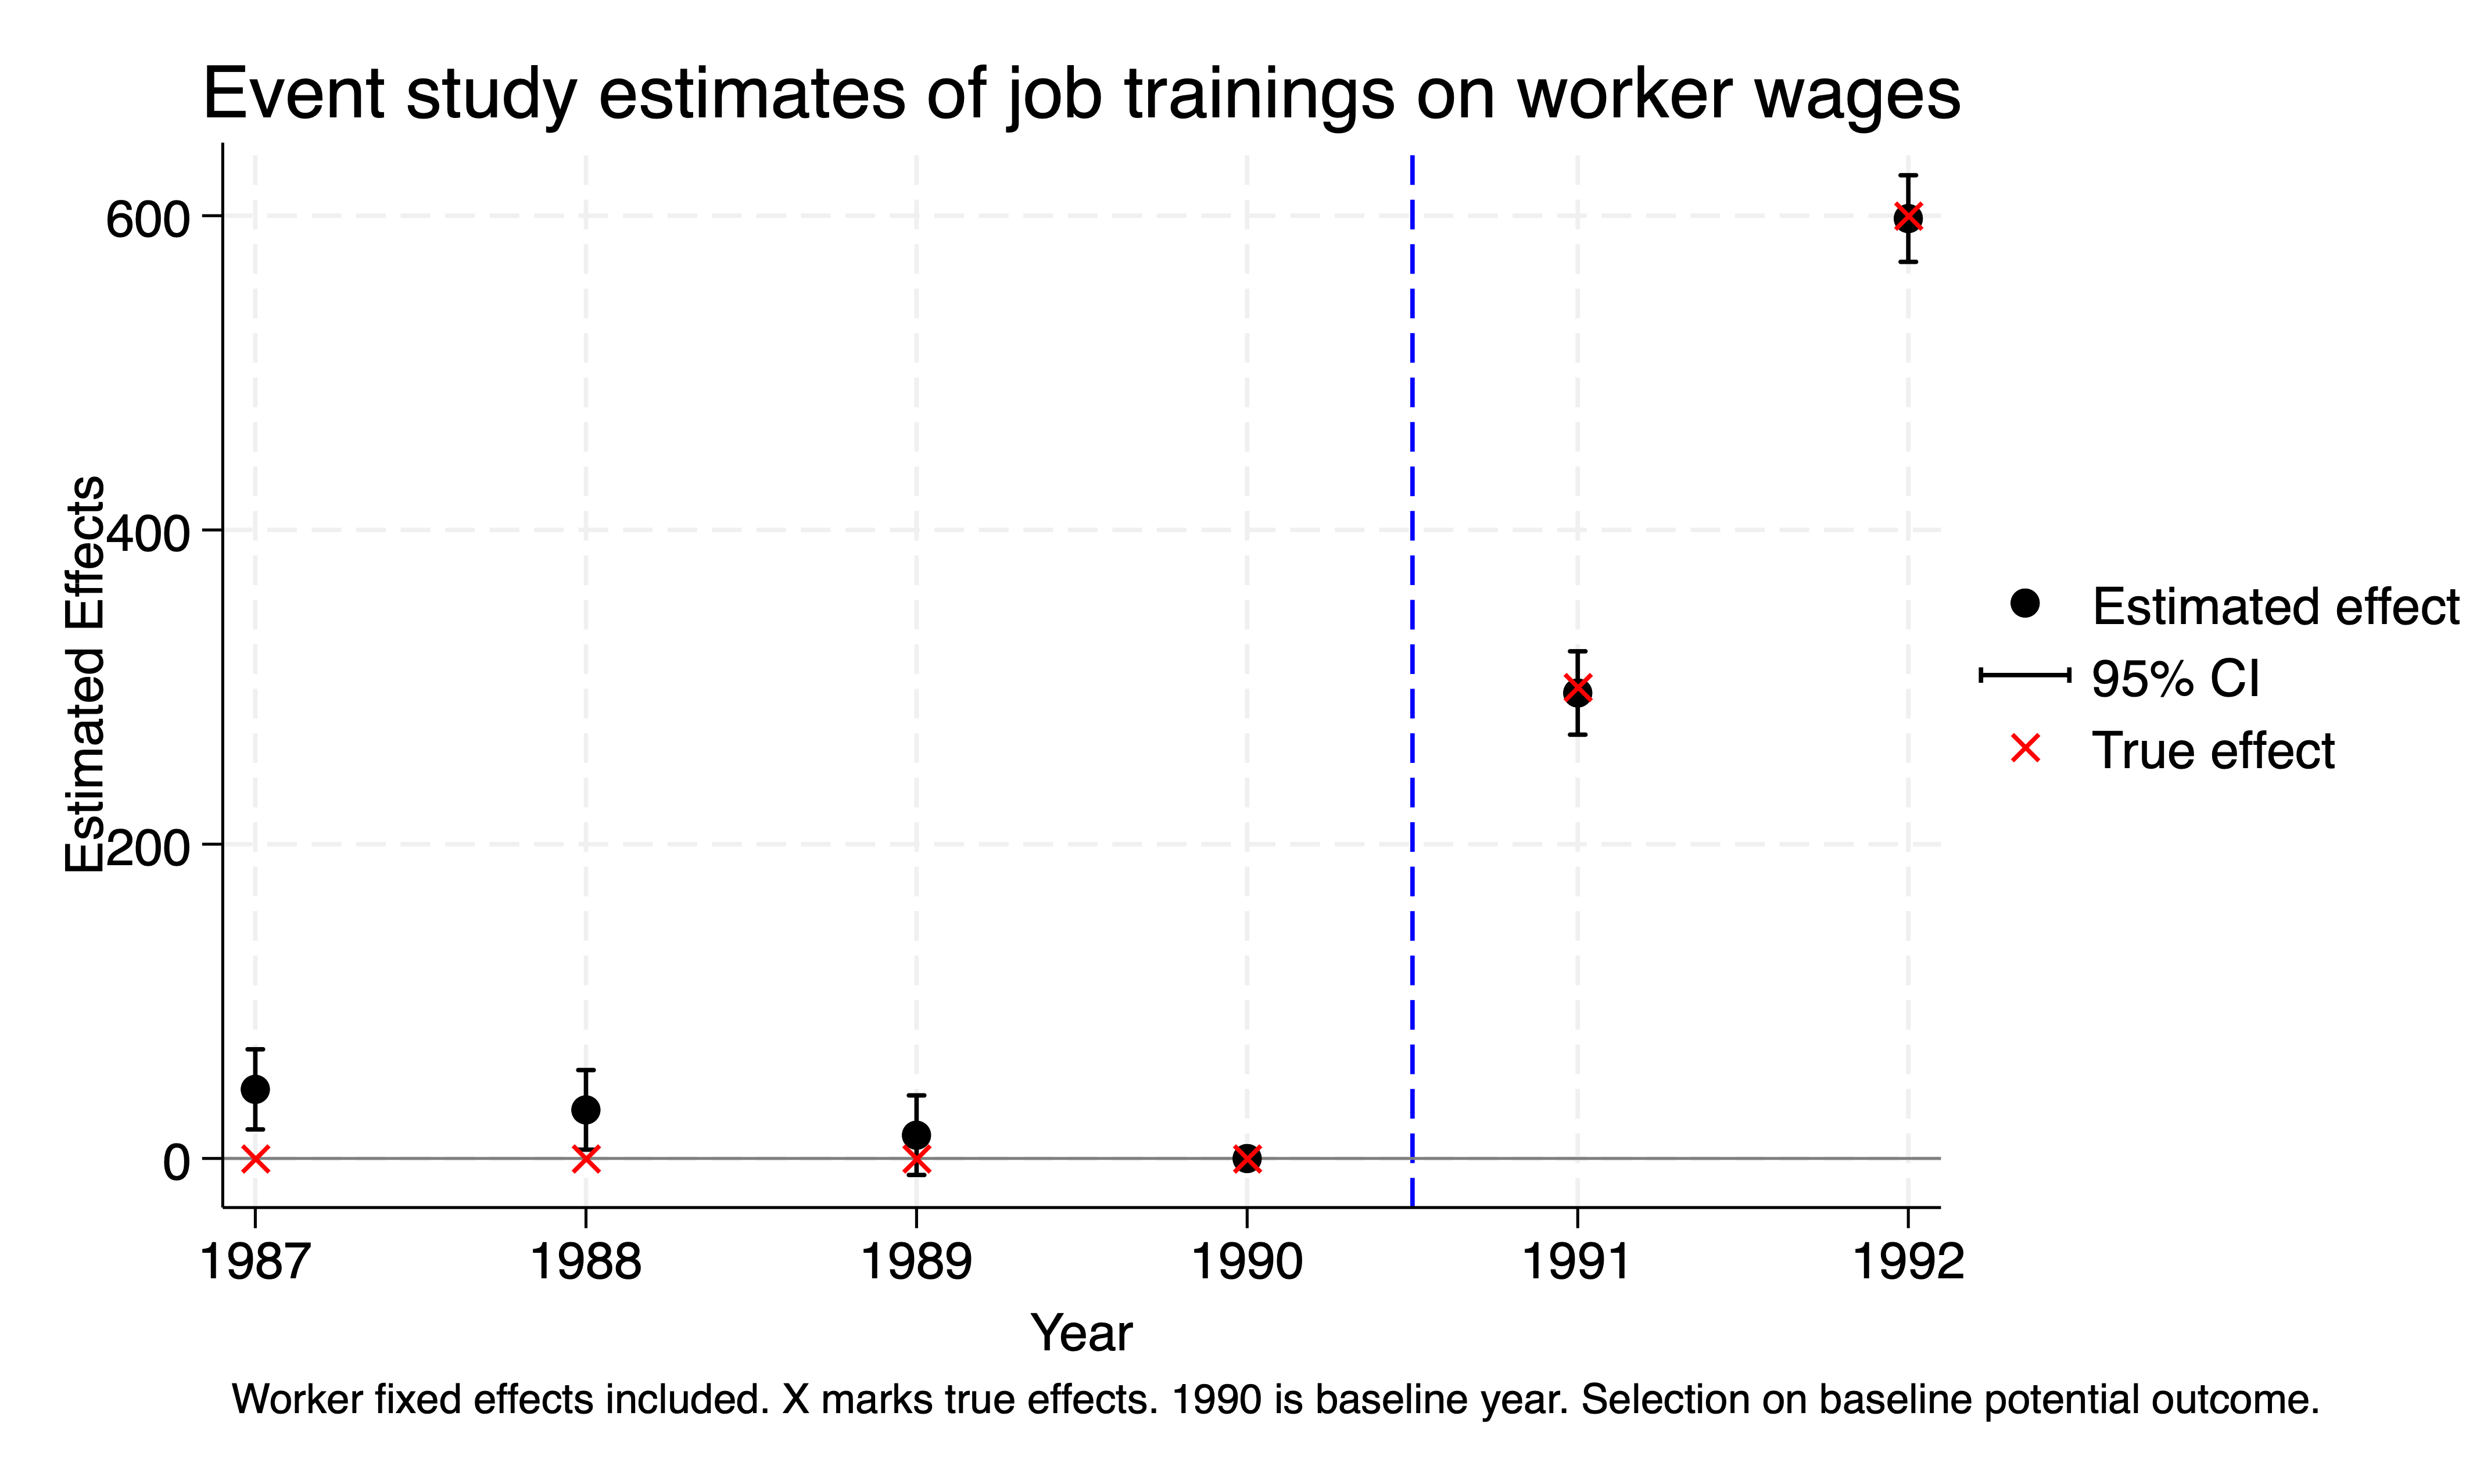
\includegraphics[width=\textwidth]{./lecture_includes/selection_y0.png}
\end{figure}

\end{frame}




\begin{frame}{Selection on observable covariates is fine}
\begin{enumerate}
    \item[3. ] \textbf{Selection on pre-treatment covariates}
    \begin{itemize}
        \item Assignment to treatment depends on observed characteristics before treatment, allowing us to condition on these covariates when assessing trends.
        \item Ex: I went to college because my parents went to college
        \item But you will need to address this in your estimation method (more on this later)
	\item See \texttt{selection_covariates} in Stata and R in /labs/selection
    \end{itemize}
    
    
\end{enumerate}
\end{frame}


\begin{frame}
 
\begin{figure}
    \centering
    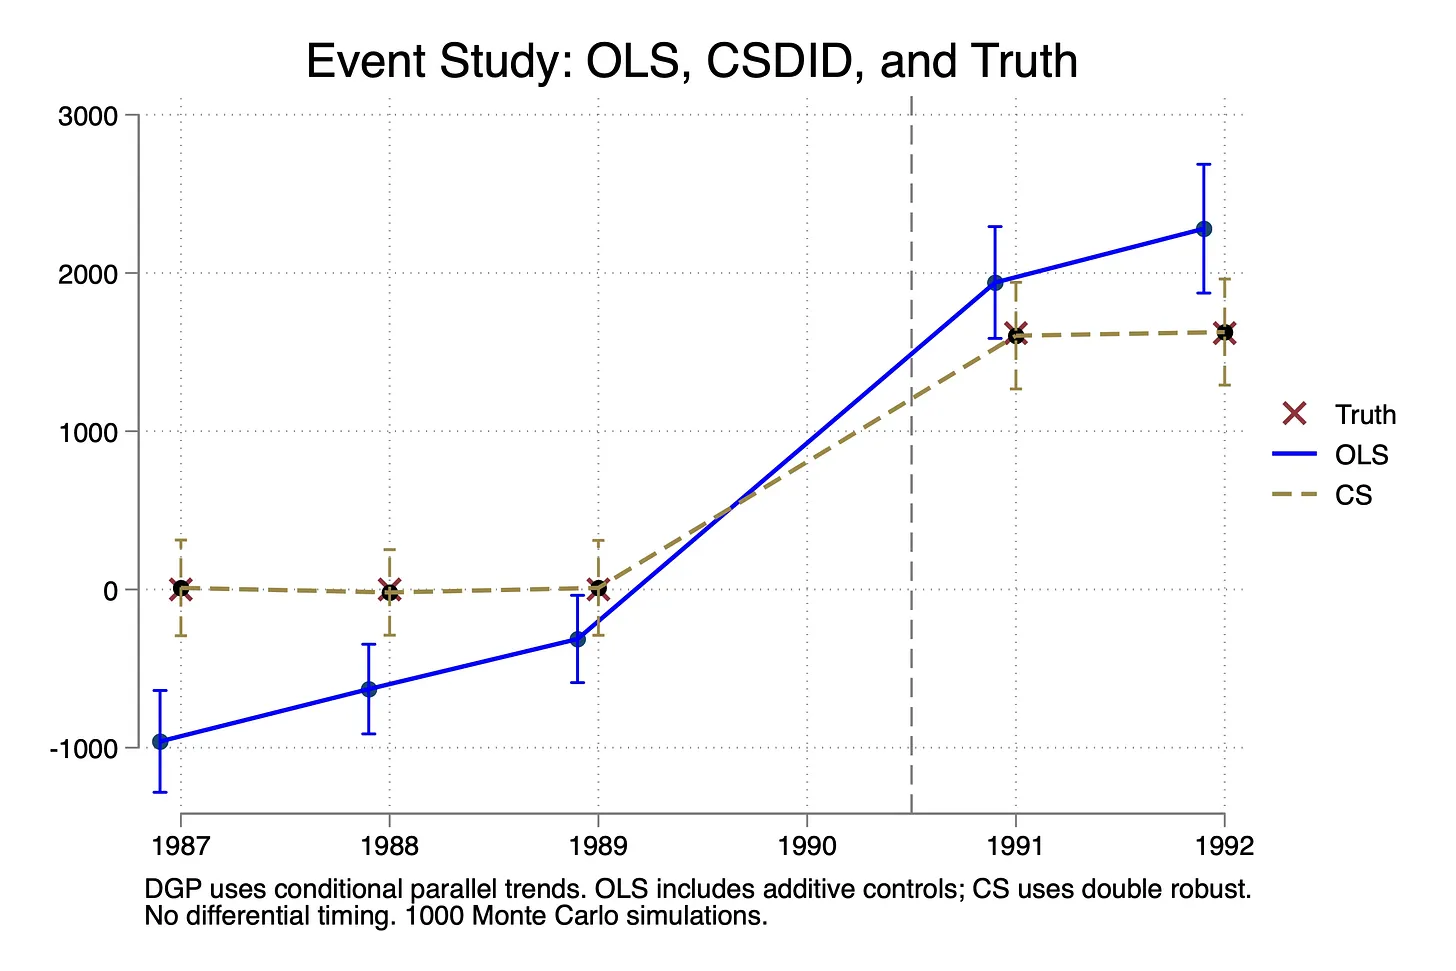
\includegraphics[width=\textwidth]{./lecture_includes/selection_covariates}
\end{figure}

\end{frame}


\begin{frame}{Selection on fixed characteristics is fine}
\begin{enumerate}
    
    \item[4. ] \textbf{Selection on fixed effects}
    \begin{itemize}
        \item Treatment is assigned based on characteristics that do not change over time, such as inherent traits or long-term conditions.
        \item Ex: I went to college because I was born in 1975
        \item See \texttt{selection_fe} in Stata and R in /labs/selection
    \end{itemize}
    
\end{enumerate}
\end{frame}

\begin{frame}
 
\begin{figure}
    \centering
    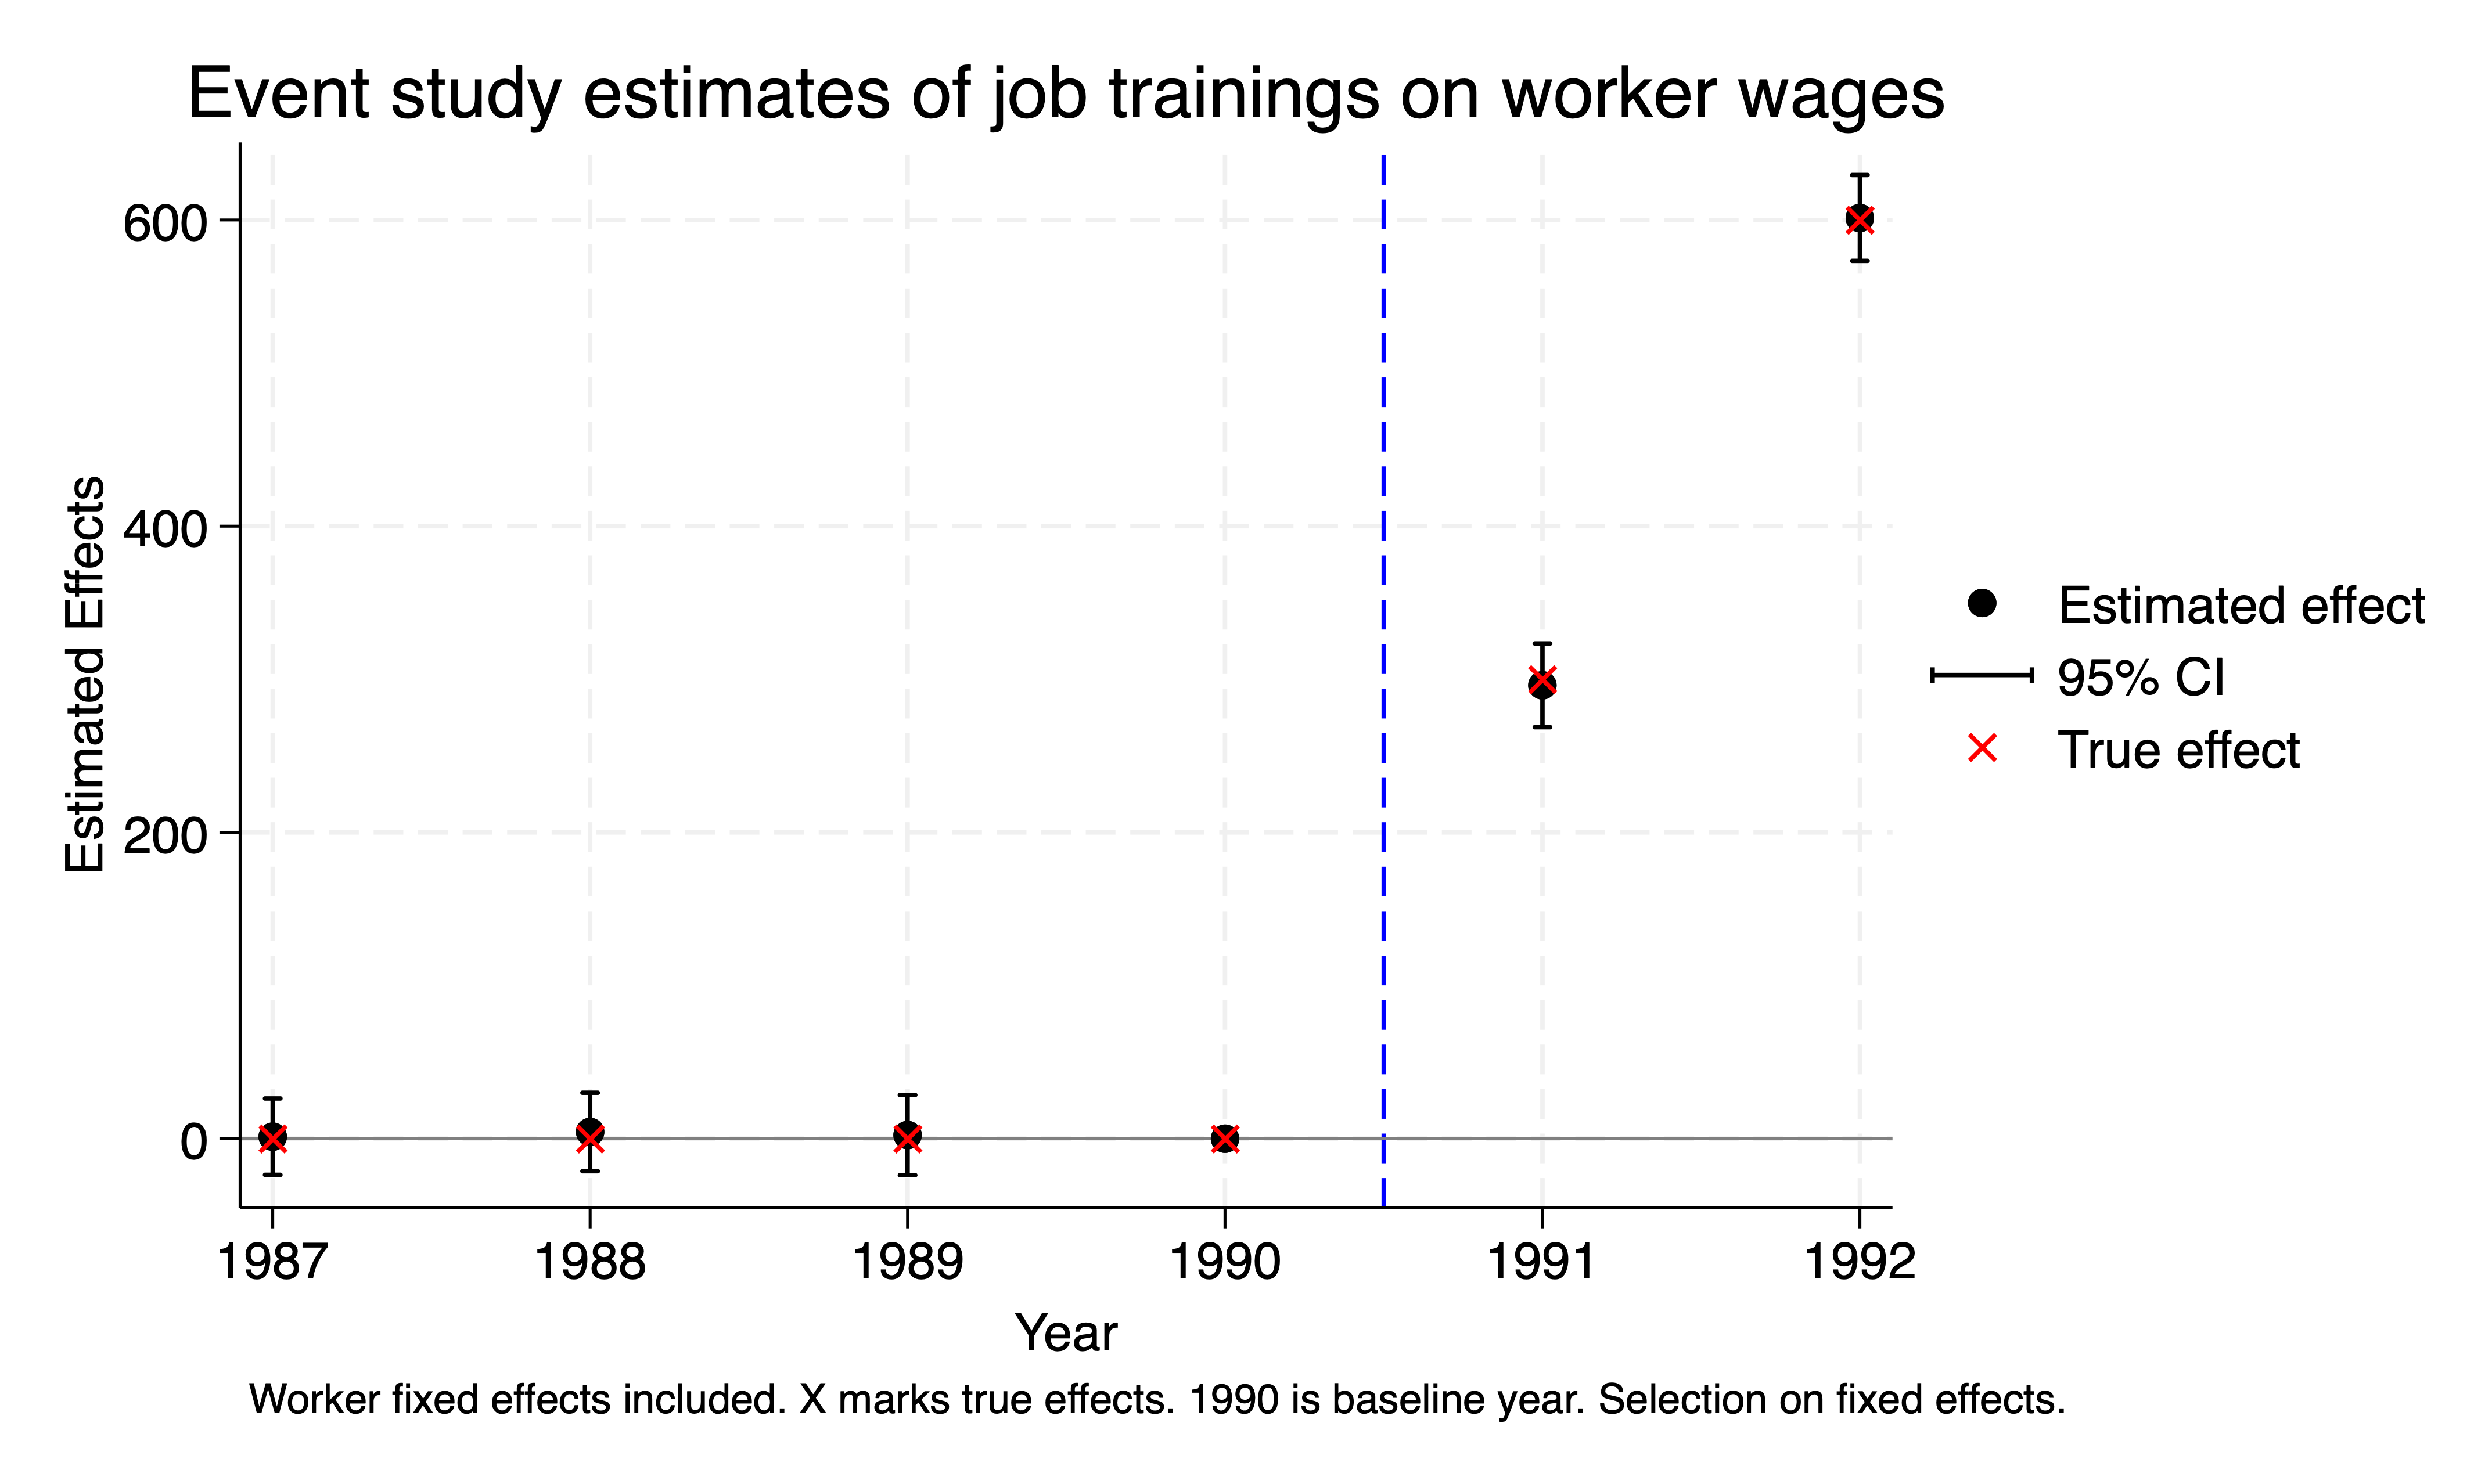
\includegraphics[width=\textwidth]{./lecture_includes/selection_fe.png}
\end{figure}

\end{frame}







\begin{frame}{Even selection on dips in outcomes is fine!}
\begin{enumerate}
    
    \item[5. ] \textbf{Selection on Dips $Y^0$}
    \begin{itemize}
        \item Workers who see \emph{changes} in baseline $Y^0$ from period to period does not violate parallel trends
        \item \dots But it will give you weird pre-trends
        \item Ex: I went to college because the year before, I saw my earnings drop by a lot
        \item See \texttt{selection_dip} in /labs/selection
    \end{itemize}
    
\end{enumerate}
\end{frame}



\begin{frame}
 
\begin{figure}
    \centering
    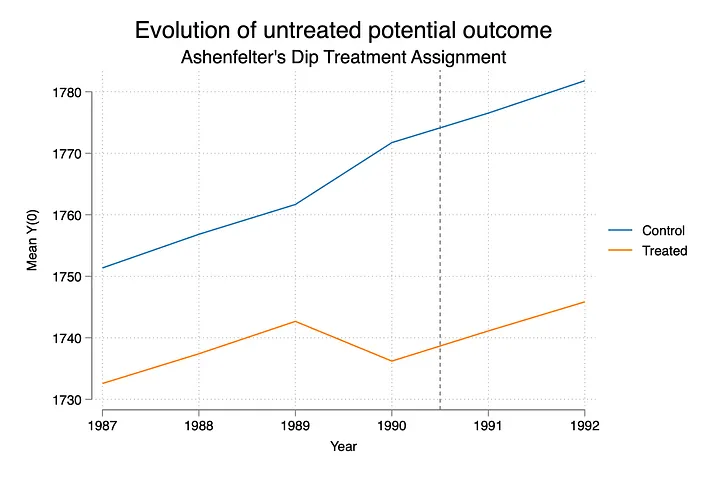
\includegraphics[width=\textwidth]{./lecture_includes/ashenfelter_po}
\end{figure}

\end{frame}

\begin{frame}
 
\begin{figure}
    \centering
    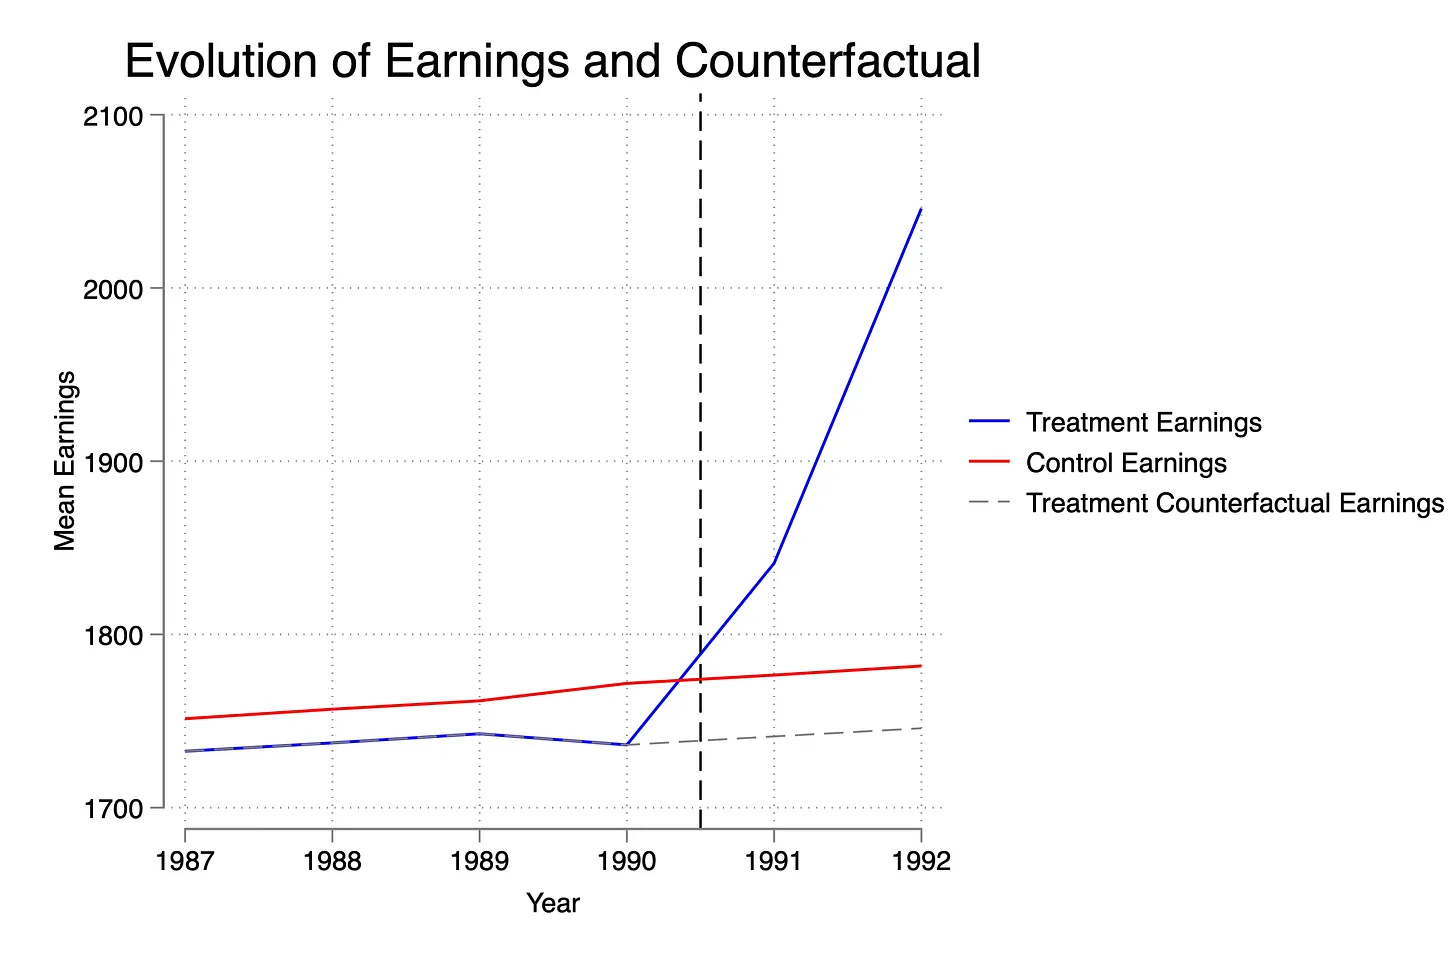
\includegraphics[width=\textwidth]{./lecture_includes/ashenfelter_y0b}
\end{figure}

\end{frame}




\begin{frame}
 
\begin{figure}
    \centering
    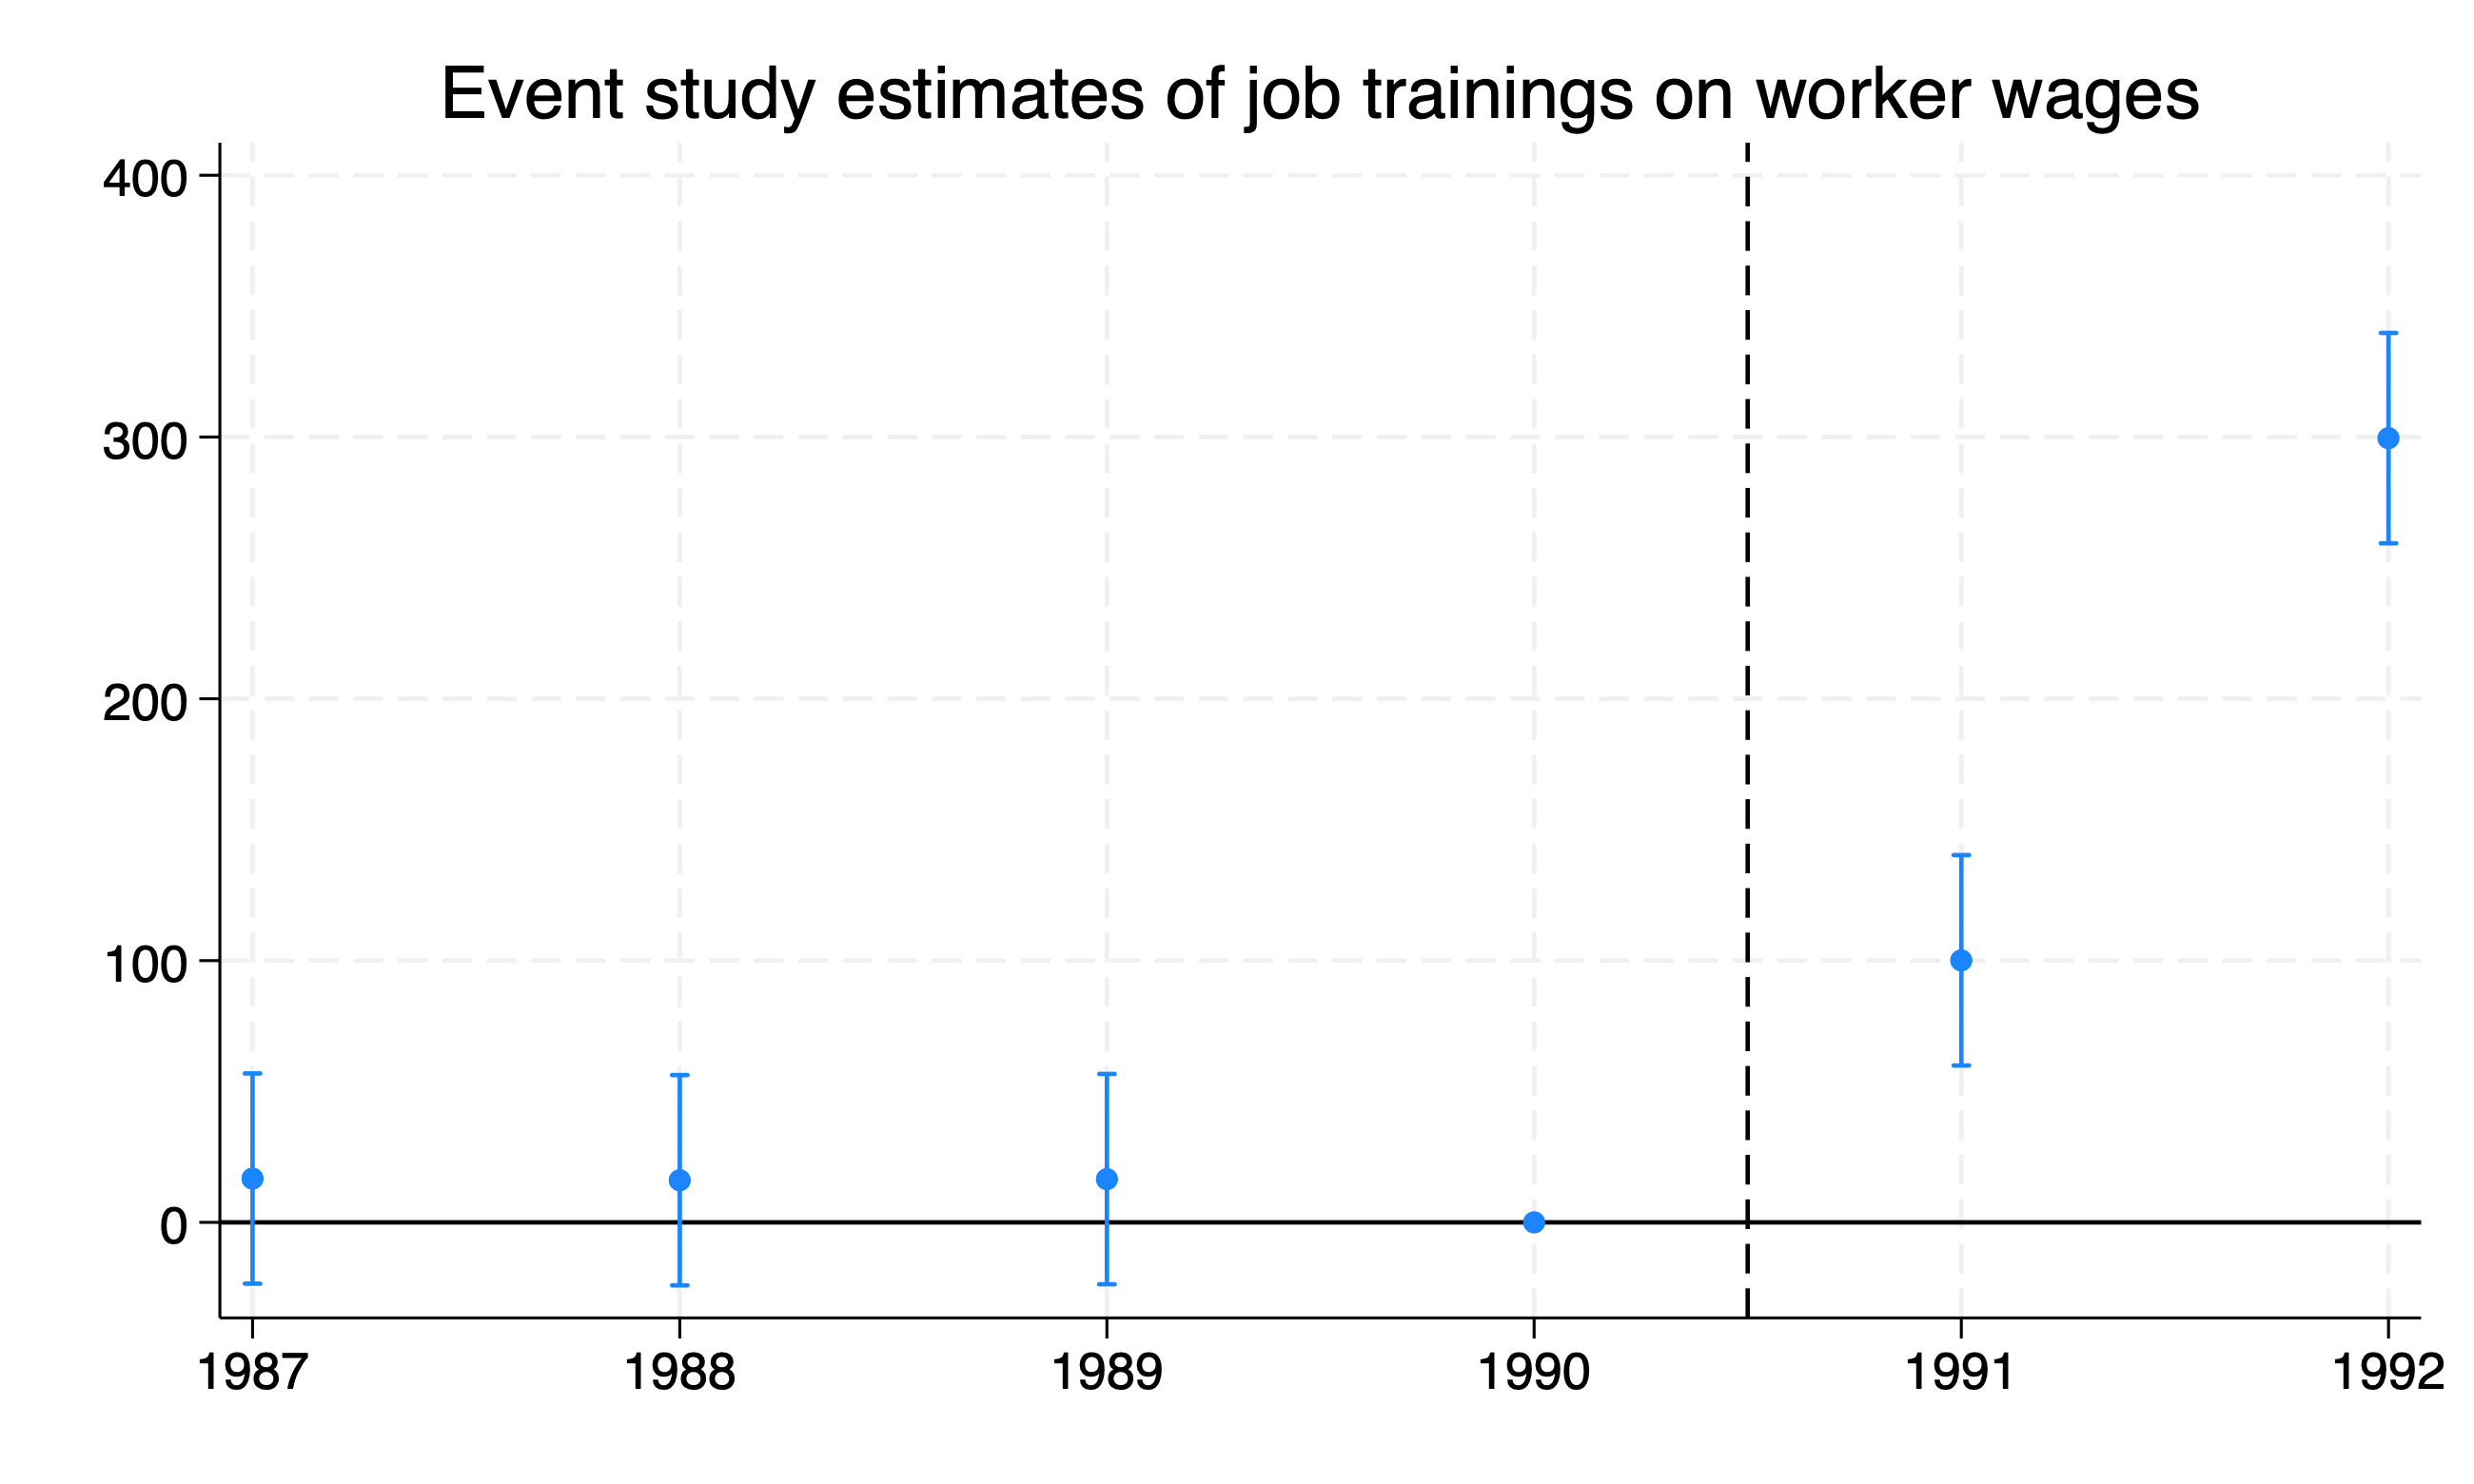
\includegraphics[width=\textwidth]{./lecture_includes/dip_es}
\end{figure}

\end{frame}


\begin{frame}{Some other stuff are also fine}
\begin{enumerate}
    
    \item[6. ] \textbf{Selection on imperfect beliefs about returns}
    \begin{itemize}
        \item Units select into treatment based on their expectations, which may not be accurate. 
        \item This can create an imperfect belief-based selection.
        \item It's when they sort into treatment based on \emph{perfect} foresight that it is a problem
    \end{itemize}
    
    \item[7. ] \textbf{Martingale property}
    \begin{itemize}
        \item The change in outcomes follows a martingale process, where future changes in unobservable factors are independent of past ones, under certain selection conditions.
    \end{itemize}
\end{enumerate}
\end{frame}


\begin{frame}{What We Should Be Concerned About}

\begin{itemize}
    \item \textbf{Time-varying unobservables}
    \begin{itemize}
        \item Unobservable factors that change over time can create biases if they affect treated and control groups differently.
        \item This can lead to violations of the parallel trends assumption if such unobservables are correlated with treatment.
    \end{itemize}
    
\end{itemize}
\end{frame}



\begin{frame}{What We Should Be Concerned About}

    \begin{itemize}
    \item \textbf{Selection based on Treatment Effects}
    \begin{itemize}
        \item If individuals select into treatment based on information they gain after the treatment starts (foresight), this undermines the assumption.
        \item Essential heterogeneity means that the potential outcomes vary systematically with unobserved traits, which complicates inference.
        \item Ex: I went to college because I knew it would cause my earnings to go up, but others didn't because they knew it would cause their earnings to fall
        \item See \texttt{selection_roy} in the /labs/selection for a simulation
    \end{itemize}
    \end{itemize}
    
\end{frame}


\begin{frame}
 
\begin{figure}
    \centering
    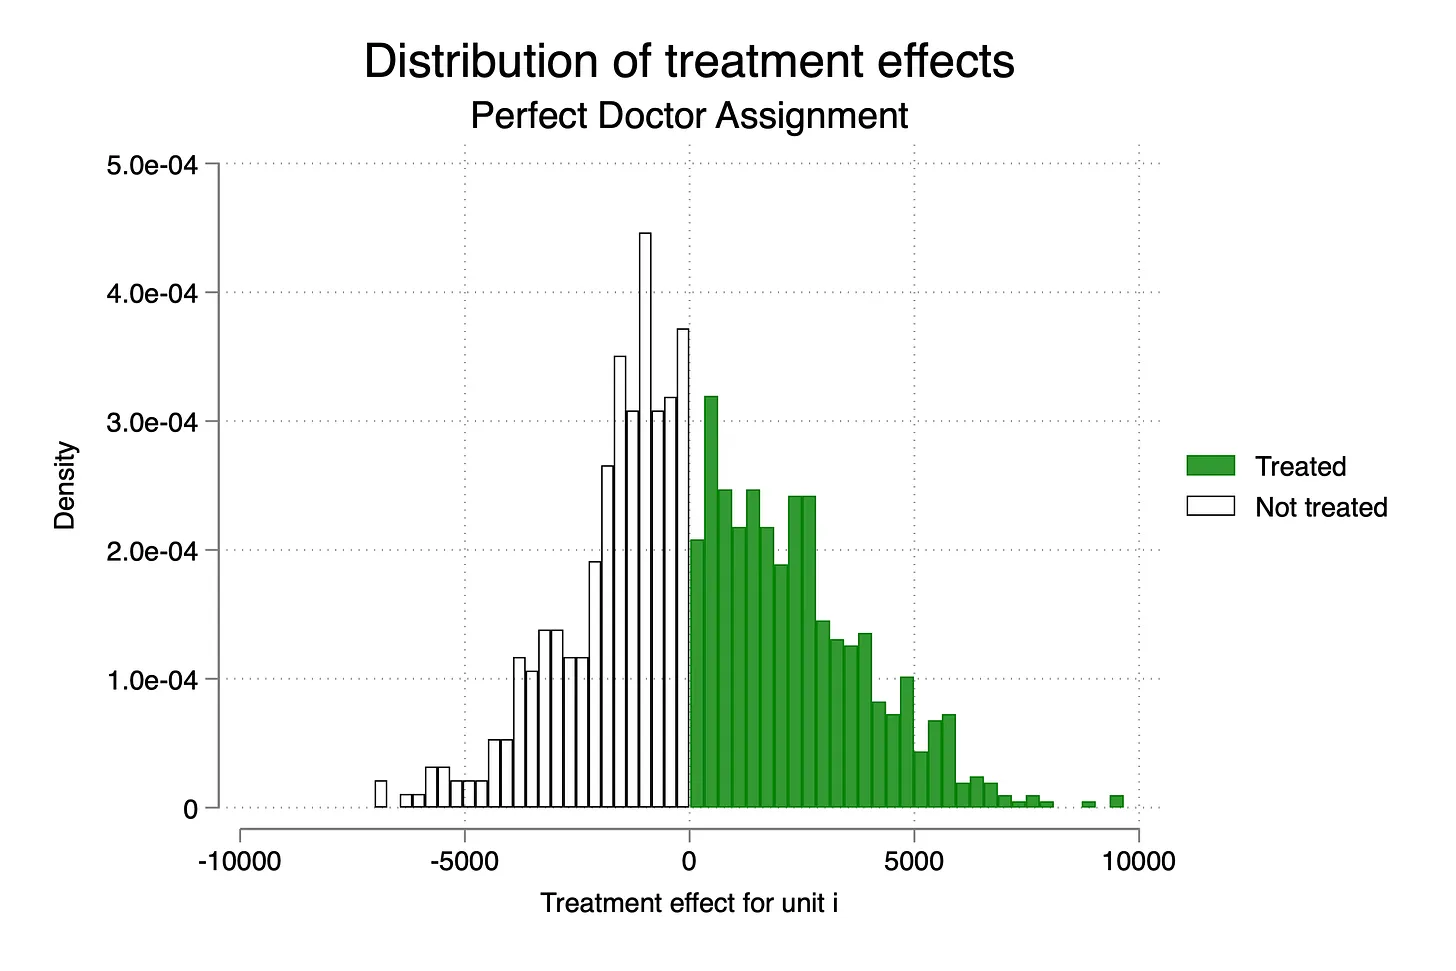
\includegraphics[width=\textwidth]{./lecture_includes/selection_te}
\end{figure}

\end{frame}

\begin{frame}
 
\begin{figure}
    \centering
    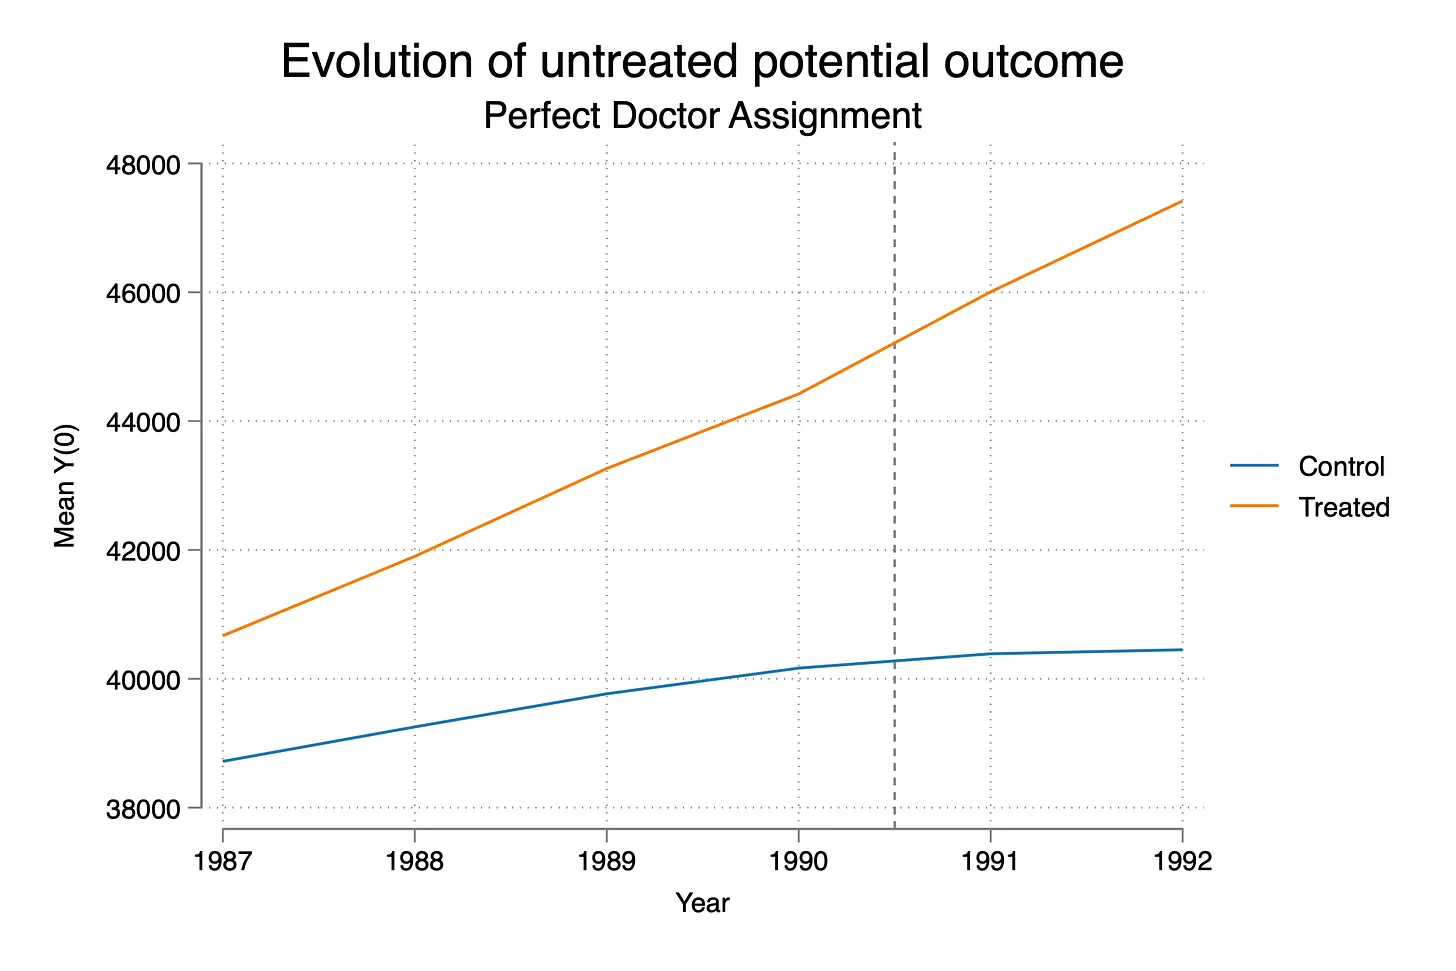
\includegraphics[width=\textwidth]{./lecture_includes/roy_diverging_po}
\end{figure}

\end{frame}





\begin{frame}
 
\begin{figure}
    \centering
    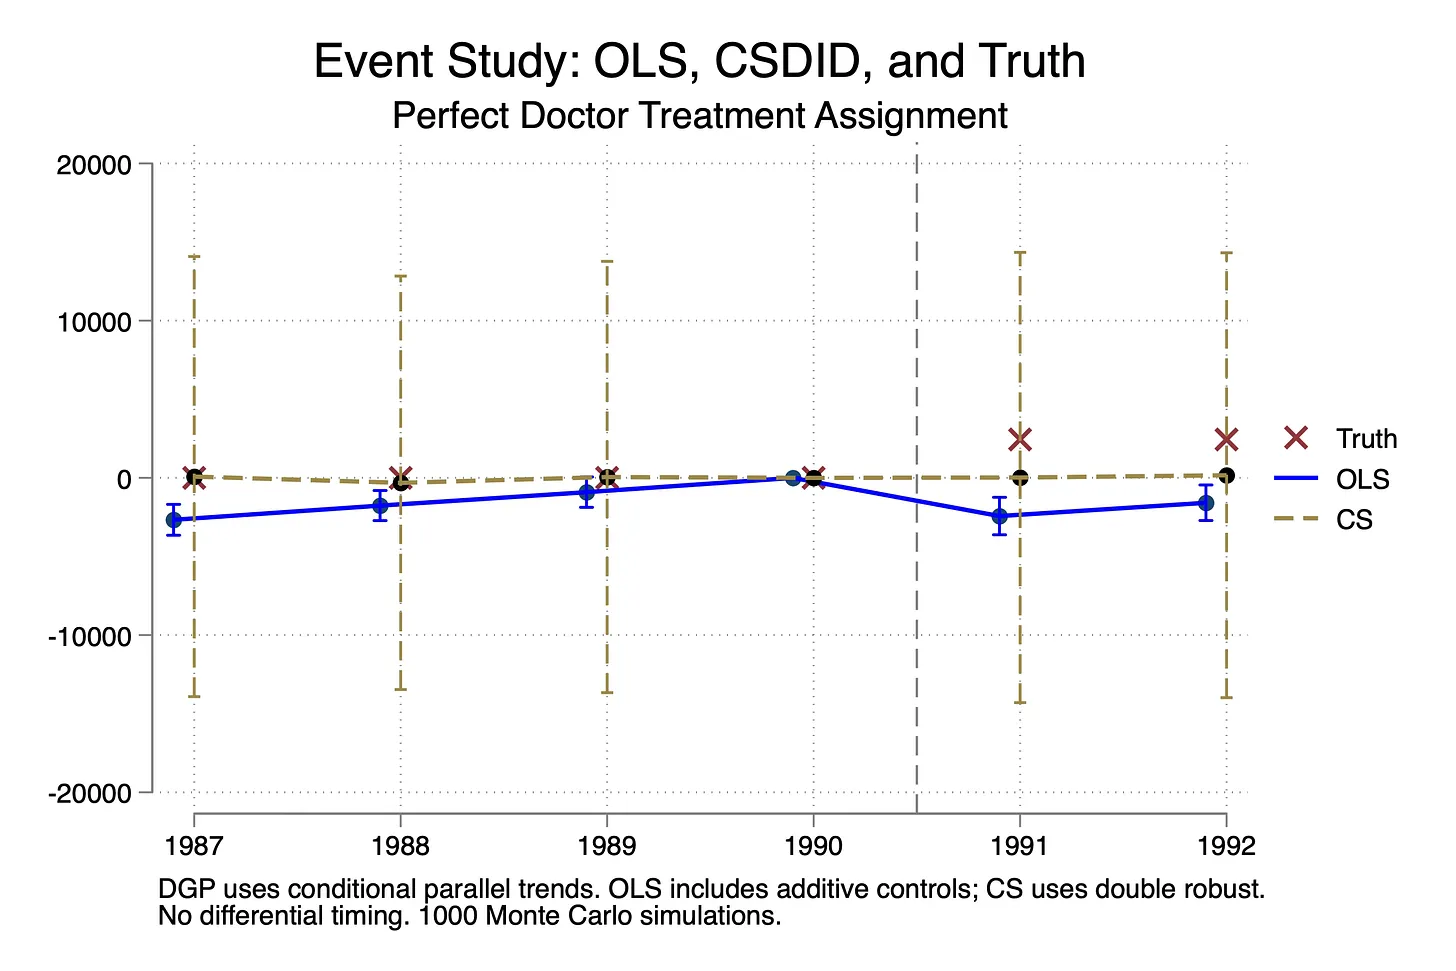
\includegraphics[width=\textwidth]{./lecture_includes/selection_roy}
\end{figure}

\end{frame}




\begin{frame}{Some other stuff aren't fine}

\footnotesize
\begin{itemize}
    
    \item \textbf{Non-stationarity}
    \begin{itemize}
        \item Non-stationarity refers to changing relationships between covariates and outcomes over time, which can lead to inconsistent treatment effect estimates.
        \item Trends in the data that are not stable or stationary across time are particularly problematic.
    \end{itemize}
    
    \item \textbf{Martingale property violation}
    \begin{itemize}
        \item If the unobservable shocks affecting outcomes do not follow a martingale process, meaning future changes are not independent of past outcomes, the model's assumptions may fail.
        \item This can result in time-dependent correlations in unobservable factors that distort trend comparisons.
    \end{itemize}
\end{itemize}
\end{frame}




\begin{frame}
 
\begin{figure}
    \centering
    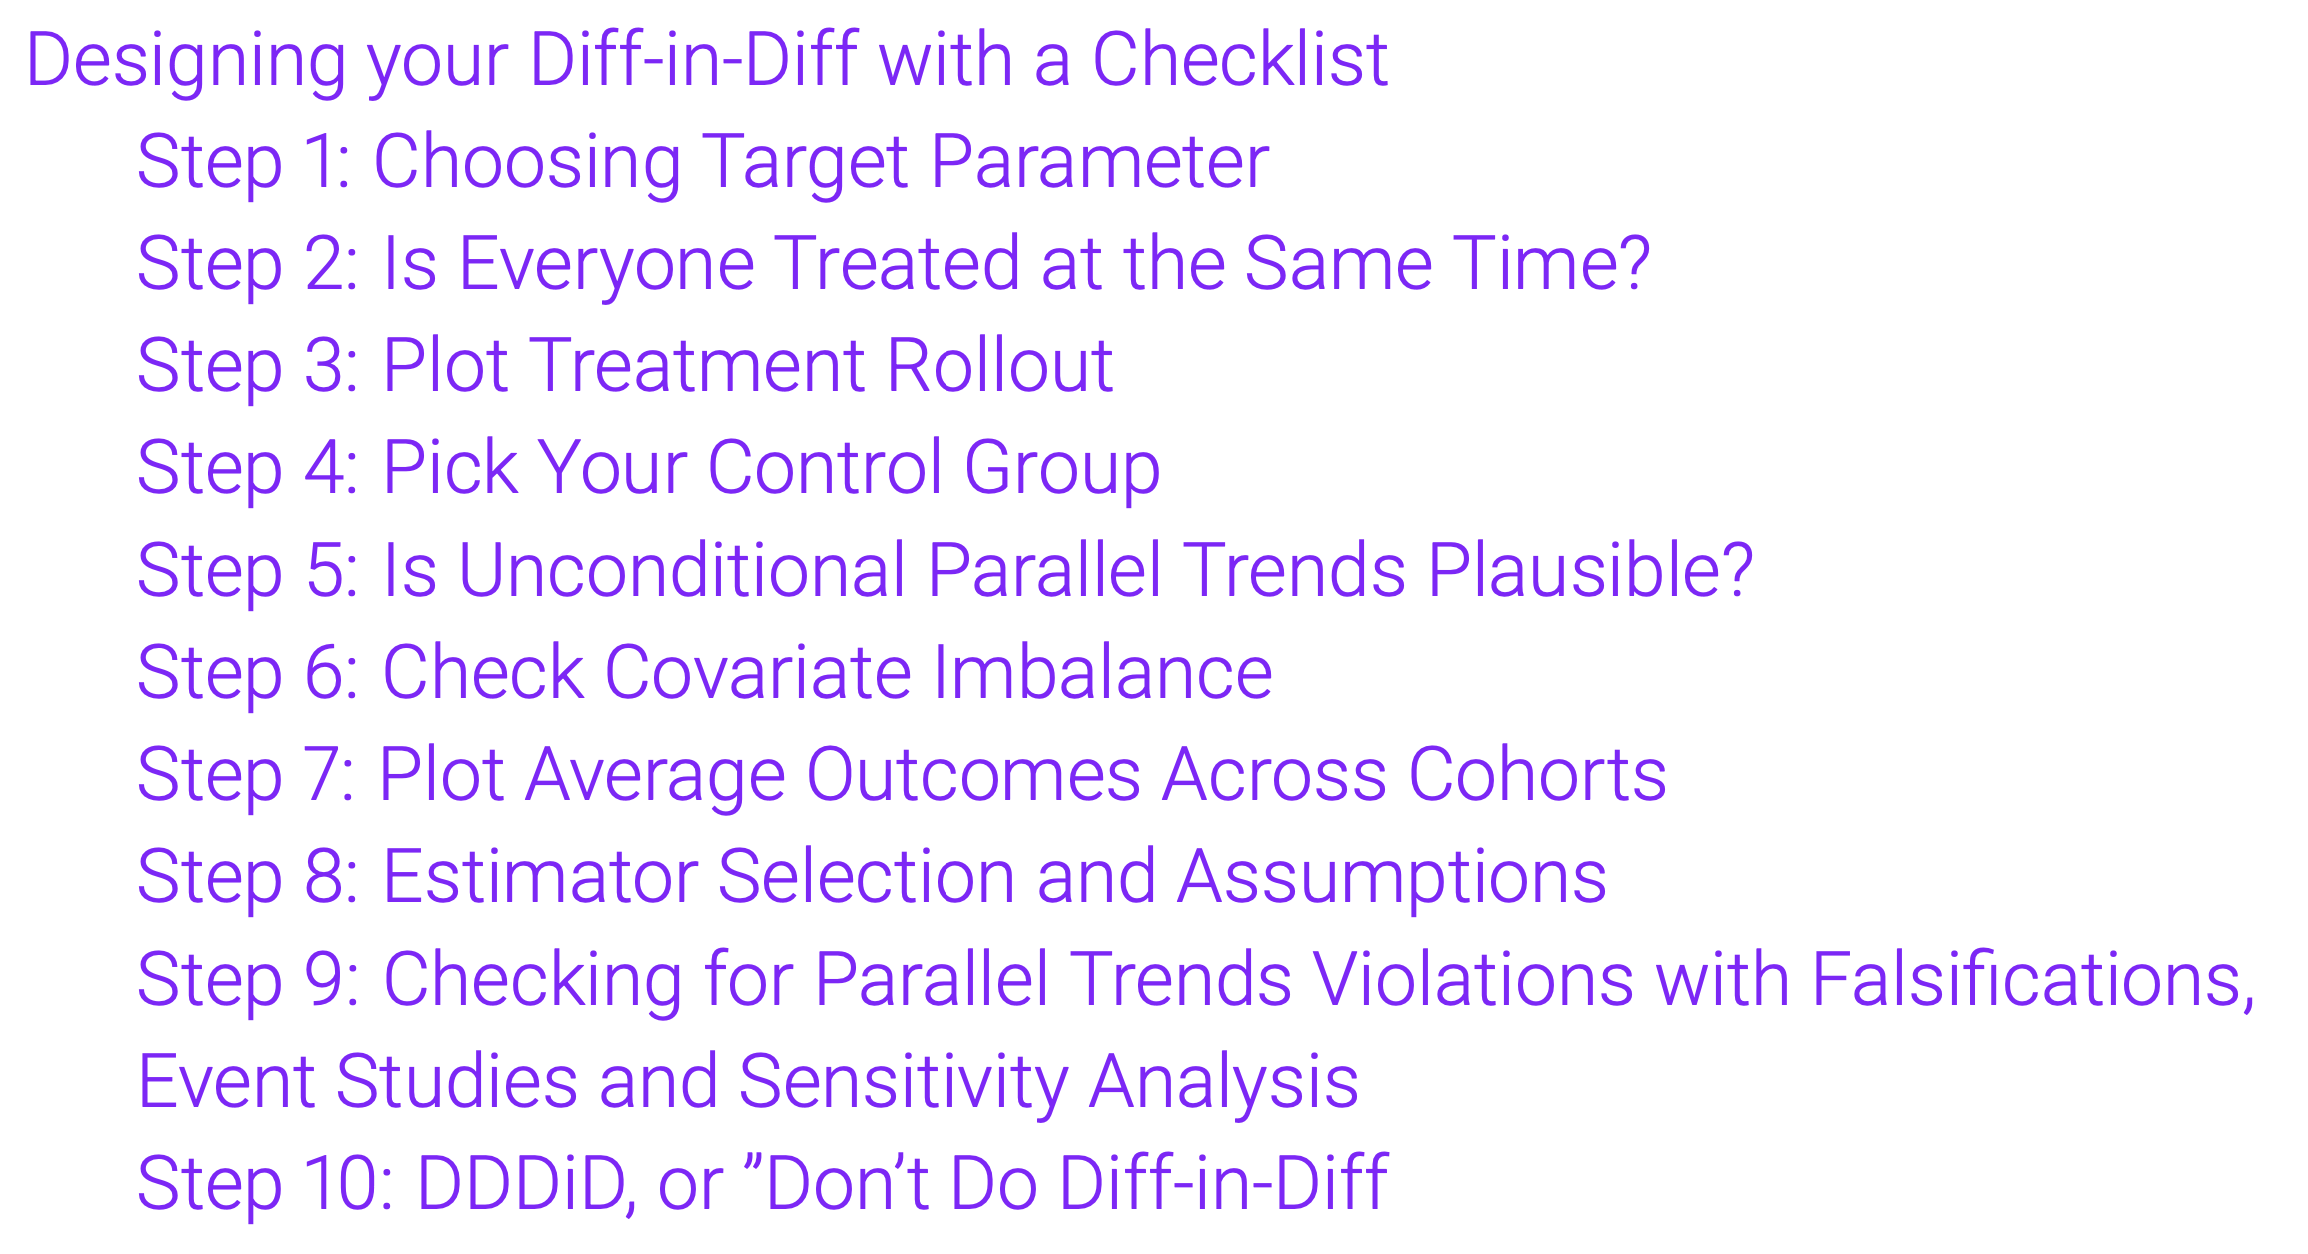
\includegraphics[width=\textwidth]{./lecture_includes/checklist}
\end{figure}

\end{frame}

\begin{frame}{Step 5: Is Unconditional Parallel Trends Plausible?}

\begin{itemize}
\item We drew a bunch of event study graphs, which leads into the next issue regarding "unconditional parallel trends"
\item Unconditional parallel trends is diff-in-diff on $Y^0$ in which the diff-in-diff equals zero
	$$\textcolor{red}{\Delta E[Y^0|D=1]} - \Delta E[Y^0|D=0] = 0$$ 
\item There are two kinds of parallel trends: unconditional and conditional
\item Let's look at a couple of spreadsheets to illustrate precisely what unconditional parallel trends mean
\end{itemize}

\bigskip 

\url{https://docs.google.com/spreadsheets/d/1onabpc14JdrGo6NFv0zCWo-nuWDLLV2L1qNogDT9SBw/edit?usp=sharing}

\end{frame}



\begin{frame}{Unconditional Parallel Trends}

\begin{itemize}
\item Unconditional parallel trends is very close to assuming that the the treatment was as good as random
\item It is not testable, but suspicion is raised when pre-treatment levels are very different as that implies non-random treatment assignment mechanisms
\item Typically, people will evaluate their parallel trends assumptions using two things:
	\begin{enumerate}
	\item Event study graphical plots of pre-trends and post-trends
	\item Falsifications on same outcomes, and similar, but untreated, groups
	\item Falsifications on different impossible outcomes, but same treatment groups
	\end{enumerate}
\item Think of these are more like 'preponderance of evidence' than proof as parallel trends \emph{cannot} be tested and graphs can be misleading
\end{itemize}


\end{frame}



\begin{frame}{Intuition behind event studies}

\begin{itemize}

	\item We cannot directly verify parallel trends, so for a long time researchers have focused on the pre-trends (e.g., Ashenfelter's Dip)
	\item \textcolor{blue}{Parallel pre-trends} are not the same as \textcolor{red}{parallel counterfactual post-trends}, but this is the smoking gun we typically look for nonetheless
	\item Think of it as a type of check for selection bias, but imperfect with false positives and false negatives
	\item Even if pre-trends are the same one still has to worry about other policies changing at the same time (omitted variable bias is a parallel trends violation)

\end{itemize}

\end{frame}



\begin{frame}{Creating event studies}

\begin{itemize}

\item You want to visualize a particularly set of regression coefficients which we will show
\item But if you can show the raw data, do that too as that will show difference in levels as well which will matter for the next section on covariates

\end{itemize}

\end{frame}



\begin{frame}

	\begin{figure}
	\includegraphics[scale=2.5]{./lecture_includes/waldinger_dd_6.pdf}
	\end{figure}

\end{frame}


\begin{frame}{Event study regression}
	
	\begin{itemize}
	\item Alternatively, present estimated coefficients from a dynamic regression specification:
 $$Y_{its} = \alpha + \sum_{\tau=-2}^{-q}\mu_{\tau} (D_s \times \tau_t) + \sum_{\tau=0}^m\delta_{\tau} (D_s \times \tau_t) + \tau_t + D_s + \varepsilon_{ist}$$
		\begin{itemize}
		\item With a simple 2x2, you are interacting treatment indicator with calendar year dummies
		\item Includes $q$ leads (dropping the $t-1$ as baseline) and $m$ lags 
		\item Since treatment did not happen until $\tau=0$, then pre-treatment coefficients only capture differential trends
		\end{itemize}
	\item Estimated $\widehat{\delta}_\tau$ coefficients are estimated ATT for each year under parallel trends but $\widehat{\mu}_\tau$ is your smoking gun evidence 
	\item Just remember that $\mu=0$ is not the same as parallel trends as parallel trends is \textcolor{red}{untestable}.
	\end{itemize}
\end{frame}

\begin{frame}{Reviewing previous slide for emphasis}


\begin{itemize}
\item Under NA, SUTVA and parallel pre-trends, then mechanically $\widehat{\mu_{\tau}}$ will be zero as everything cancels out
	\begin{itemize}
\item There are still specification and power issues that Jon Roth has written about, but I will skip that
	\end{itemize}
\item But also under NA, SUTVA and parallel trends (post trends), then $\widehat{\delta}$ are estimates of the ATT at points in time
\item  Typically you'll plot the coefficients and 95\% CI on all leads and lags
\end{itemize}

\end{frame}

\begin{frame}{Normal DiD coefficient}

\begin{eqnarray*}
\widehat{\delta} &=& \underbrace{E[Y^1_k | Post] - \textcolor{red}{E[Y^0_k | Post]}}_{\mathclap{\text{ATT}}} \\
&& + \bigg [  \underbrace{\textcolor{red}{E[Y^0_k | Post]} - E[Y^0_k | Pre] \bigg ] - \bigg [ E[Y^0_U | Post] - E[Y_U^0 | Pre] }_{\mathclap{\text{Non-parallel trends bias in 2x2 case}}} \bigg ]
\end{eqnarray*}

\bigskip

But this was \emph{post}-treatment.  Still, put that aside -- diff-in-diff equations \emph{always} identify the sum of those terms, even in the pre-period


\end{frame}

\begin{frame}{Pre-treatment DiD coefficient}

\begin{eqnarray*}
\widehat{\delta}_{t-2} &=& \bigg [  \underbrace{\textcolor{black}{E[Y^0_k | t-2]} - E[Y^0_k | t-1] \bigg ] - \bigg [ E[Y^0_U | t-2] - E[Y_U^0 | t-1] }_{\mathclap{\text{Non-parallel trends bias in 2x2 case}}} \bigg ]
\end{eqnarray*}

\bigskip

Under NA, then the $t-1$ period is untreated.  But then so are the other pre-periods so the ATT is implicitly zero and the \emph{only} thing that you can be measuring with pre-trend DiD coefficients is differential trends.  


\end{frame}



\begin{frame}{Event study coefficients}

\begin{itemize}
\item Remember that the OLS specification we discuss collapses to ATT plus parallel trends bias
\item This is \emph{always} true because it's an identity and holds even in the pre-period as much in the post
\item It's just in the pre period, you do not have the missing $E[Y^0|D=1]$ term as no one and nothing is treated in pre-period under NA
\item This means pre-period is basically an opportunity to directly verify parallel pre-trends -- but it's the past's pre-trends, not the counterfactual pre-trend of the present/future
\item And that's how people use the pre-period -- they use the pre-period to evaluate whether they think this is a good control group
\end{itemize}

\end{frame}

\begin{frame}{Event study example}

\begin{itemize}
\item The notion is really simple: if PT held then, you'll argue that it's reasonable it would've still held
\item But this is an assertion, and you need to build the case as we said
\item At this point, it's a lot easier to show you what I'm talking about -- where the art and the science meet -- with a great paper
\end{itemize}

\end{frame}




\begin{frame}{Medicaid and Affordable Care Act example}

\begin{figure}
\includegraphics[scale=0.25]{./lecture_includes/medicaid_qje}
\end{figure}

\end{frame}
\begin{frame}{Their Evidence versus Their Result}

\begin{itemize}
\item \textbf{Bite} -- they will show that the expansion shifted people into Medicaid and out of uninsured status
\item \textcolor{black}{\textbf{Falsifications}} -- they show that there's no effect of Medicaid on a similar group that didn't enroll
\item \textbf{Event study} -- they will lean hard on those dynamic plots
\item \textcolor{red}{\textbf{Main results}} -- with all of this, they will show Medicaid expansion caused near elderly mortality to fall
\item \textcolor{black}{\textbf{Mechanisms}} -- they think they can show it's coming from people treating diseases causing mortality declines to compound over time
\end{itemize}

\end{frame}

\begin{frame}{Bite}

\begin{itemize}
\item Bite is a labor economist's phrase, often used with the minimum wage, to say that the minimum wage actually was binding in the first place
\item Here it means when US states made Medicaid more generous, people got on Medicaid who would not have been on it otherwise
\item And as a bonus, would not have been insured at all without it
\item Not the most exciting result, but imagine if the main results on mortality were shown but there was no evidence for bite -- is it believable?
\end{itemize}

\end{frame}


\imageframe{./lecture_includes/Miller_Medicaid1.png}

\imageframe{./lecture_includes/Miller_Medicaid2.png}

\imageframe{./lecture_includes/Miller_Medicaid3.png}


\begin{frame}{Falsification}

\begin{itemize}

\item Their study focuses on ``near elderly'', which means just under 65
\item They choose just under 65 because in the US, 65 and older are eligible for Medicare so more generous Medicaid is irrelevant
\item \emph{But} probably the near elderly and the elderly are equally susceptible to unobserved factors correlated with the treatment
\item So they painstakingly examine the effects on elderly as a falsification as this will strengthen the parallel trends assumption on the near elderly
\end{itemize}

\end{frame}

\begin{frame}{Falsifications on elderly}

	\begin{figure}
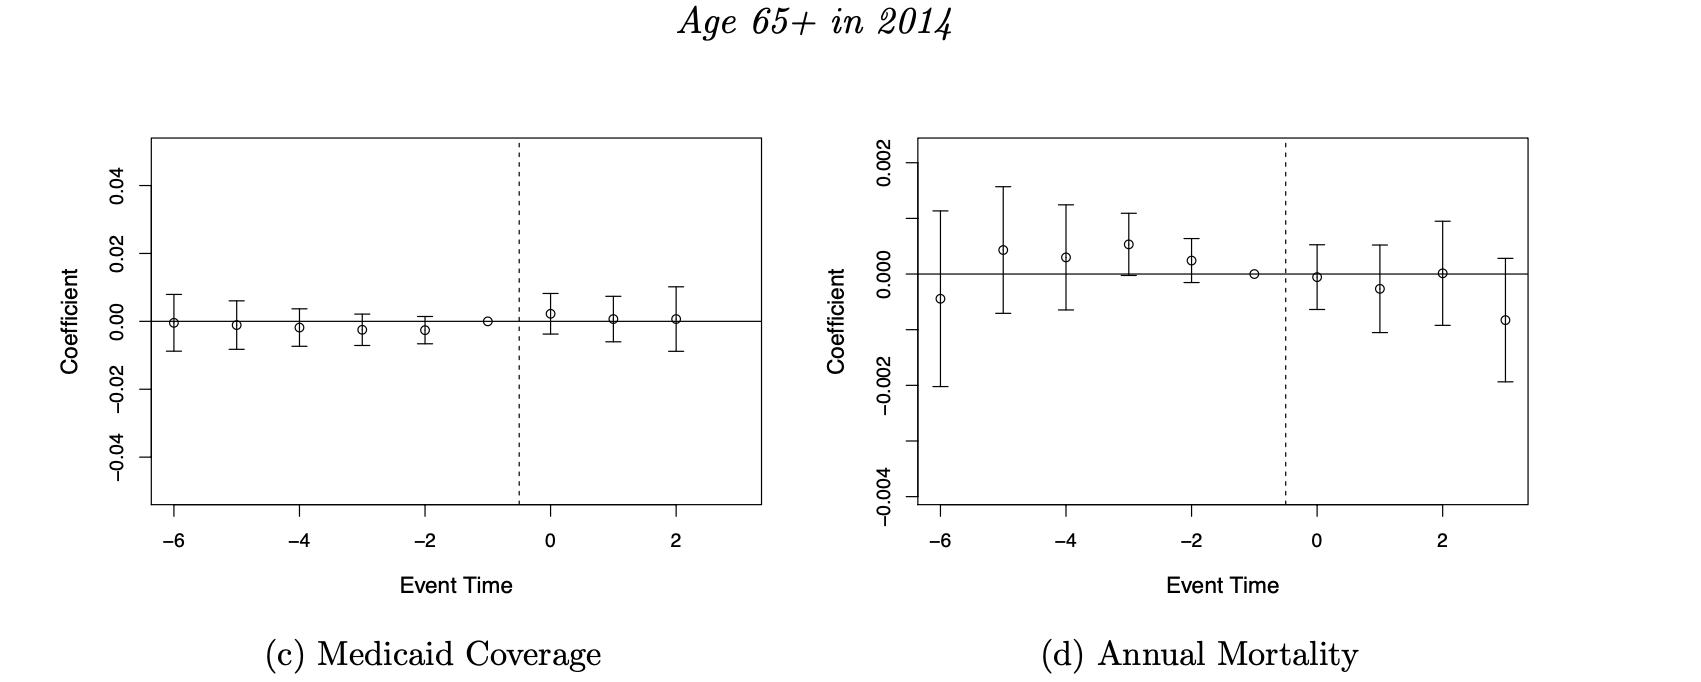
\includegraphics[scale=0.425]{./lecture_includes/placebo_medicaid}
	\end{figure}

\end{frame}

\begin{frame}{Main result}

\begin{itemize}

\item Finally they focus on the main result -- and there's more in the paper than I'm showing
\item Event study plots with same specification as the rest allowing us to look at the pre-trends and the post-treatment coefficients
\item If parallel trends holds, then the post-treatment coefficients are interpreted as ATT parameter estimates for each time period
\item The result alone isn't nearly as strong the result in combination with the rest, but it could still be wrong as parallel trends is ultimately not verfiable
\end{itemize}

\end{frame}



\begin{frame}{Near elderly mortality and Medicaid expansion}

	\begin{figure}
	\includegraphics[scale=0.3]{./lecture_includes/Miller_Medicaid4.png}
	\end{figure}

\end{frame}

\begin{frame}{Summarizing evidence and results}

\begin{itemize}
\item \textbf{Bite}: Increases in enrollment and reductions in uninsured support that there is adoption of the treatment
\item \textbf{Event studies}: Compelling graphics showing similarities between treatment and control
\item \textbf{Falsifications}: no effect on a similar group who isn't eligible
\item \textcolor{red}{Main results}: 9.2\% reduction in mortality among the near-elderly
\item \textcolor{red}{Mechanism}: ``The effect is driven by a reduction in disease-related deaths and grows over time.''
\end{itemize}

\end{frame}

\begin{frame}{Making event study}

\begin{itemize}
\item When there is only one treatment group and one comparison group, then you run a regression with an interaction of the treatment group dummy and the calendar year dummies (plus both separately)
\item You must drop $t-\tau$ as the baseline (e.g., $t-1$) and it must be $Y^0$ untreated comparisons (No Anticipation)
\item I have included in a do file that will do it for you either manually or using coefplot in \texttt{simple\_eventstudy.do} at the shared github labs directory
\end{itemize}

\end{frame}


\begin{frame}{Manually creating the event study}

	\begin{figure}
	\includegraphics[scale=0.20]{./lecture_includes/simple_eventstudy_manual}
	\end{figure}

\end{frame}




\begin{frame}{Creating the event study with Ben Jann's \texttt{coefplot}}

	\begin{figure}
	\includegraphics[scale=0.20]{./lecture_includes/simple_eventstudy.png}
	\end{figure}

\end{frame}


\begin{frame}{Don't ask more of event studies than they can give}

\begin{itemize}
\item Event studies are mandatory -- you must make them
\item But remember, parallel trends cannot be seen in event studies -- only \emph{pre-trends} can
\item Parallel trends can be satisfied and pre-trends be messed up; pre-trends can look good, and parallel trends be violated

\end{itemize}
\end{frame}

\begin{frame}{Proof vs Evidence}

\begin{itemize}
\item Think of event studies as \emph{evidence}, not \emph{proof}
	\begin{itemize}
	\item Prosecutor based on police produces fingerprints, eyewitnesses and imprints in mud
	\end{itemize}
\item Event studies are evidence of pre-trends only, but they are consistent with various forms (but not all) forms of selection
\item Falsifications are post-treatment heuristics based on logic and counter-evidence (Popperian reasoning)
\end{itemize}
\end{frame}



\begin{frame}{Falsification 1: same outcome, but untreated groups}
		
		\begin{figure}
		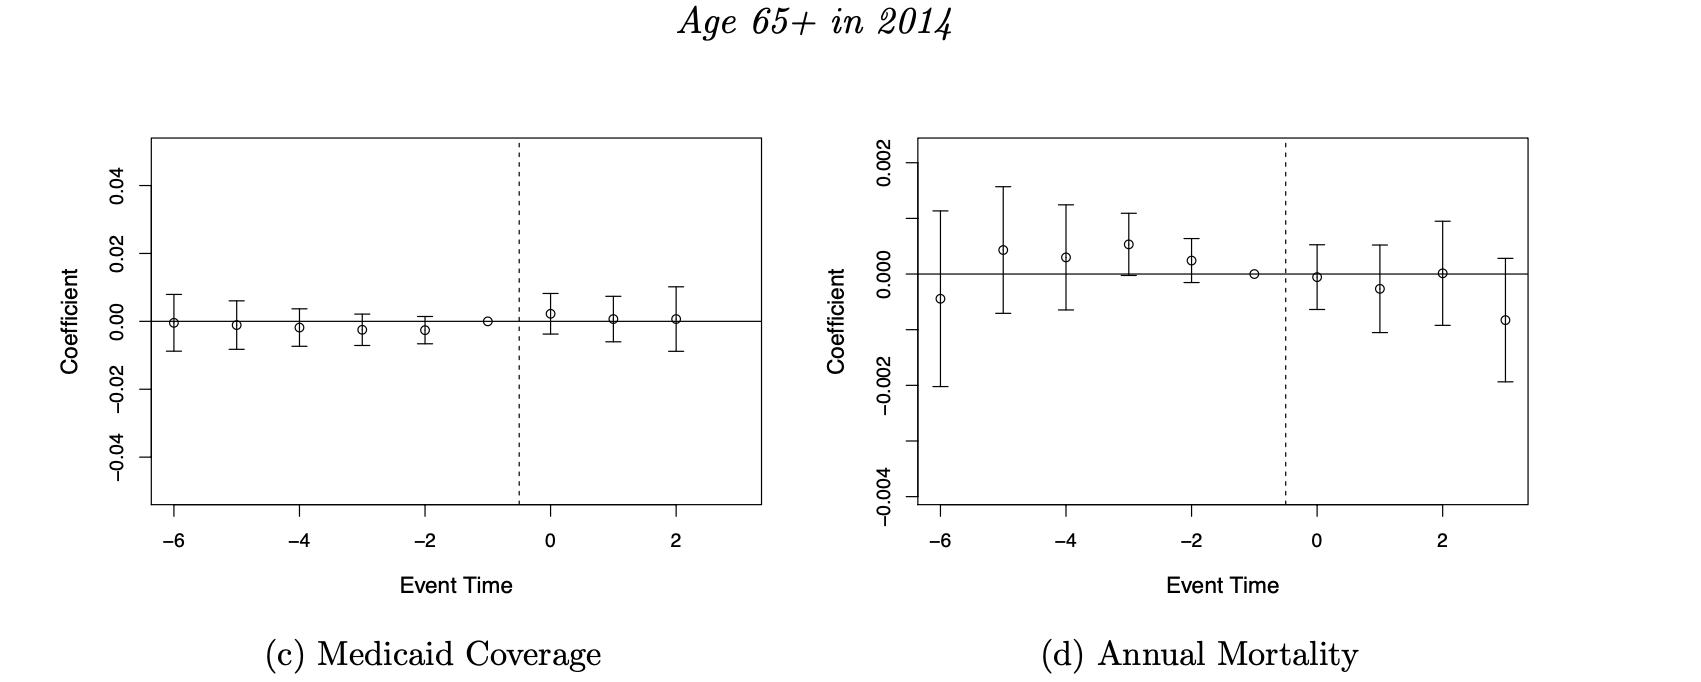
\includegraphics[scale=0.425]{./lecture_includes/placebo_medicaid}
		\end{figure}

\end{frame}

\begin{frame}{Falsification 2: different outcomes, same treatment group}
	\begin{itemize}
	\item Good falsifications make logical sense:  
		\begin{itemize}
		\item They are a similar enough group (near elderly versus elderly) 
		\item They are an outcome that would be susceptible to some omitted variable you're worried about
		\end{itemize}
	\item Two examples
		\begin{itemize}
		\item Cheng and Hoekstra (2013) examine the effect of a gun laws on non-gun related offenses like grand theft auto and find no evidence of an effect 
		\item Cunningham, DeAngelo and Tripp (2024) examine effect of a sex worker platform on irrelevant crime categories
		\end{itemize}
	\end{itemize}
\end{frame}



\begin{frame}{Rational addiction as a placebo critique}


Sometimes, an empirical literature may be criticized using nothing more than placebo analysis

\begin{quote}``A majority of [our] respondents believe the literature is a success story that demonstrates the power of economic reasoning.  At the same time, they also believe the empirical evidence is weak, and they disagree both on the type of evidence that would validate the theory and the policy implications. Taken together, this points to an interesting gap.  On the one hand, most of the respondents claim that the theory has valuable real world implications.  On the other hand, they do not believe the theory has received empirical support.''
\end{quote}

\end{frame}

\begin{frame}{Placebo as critique of empirical rational addiction}

\begin{itemize}
	\item Auld and Grootendorst (2004) estimated standard ``rational addiction'' models (Becker and Murphy 1988) on data with milk, eggs, oranges and apples.  
	\item They find these plausibly non-addictive goods are addictive, which casts doubt on the empirical rational addiction models.
\end{itemize}

\end{frame}

\begin{frame}{Placebo as critique of peer effects}

\begin{itemize}
	\item Several studies found evidence for ``peer effects'' involving inter-peer transmission of smoking, alcohol use and happiness tendencies
	\item Christakis and Fowler (2007) found significant network effects on outcomes like obesity
	\item Cohen-Cole and Fletcher (2008) use similar models and data and find similar network ``effects'' for things that \emph{aren't} contagious like acne, height and headaches
	\item Maybe tall people have tall friends because basketball players are friends with one another?
\end{itemize}

\end{frame}


\begin{frame}{Triple differences is a research design}

\begin{itemize}

\item Many people equate triple differences with falsification exercise, but actually it isn't that -- it is it's own design
\item You use triple differences when you have a parallel trends violation -- that is, when your diff-if-diff is biased
\item Triple differences may sound like a falsification, but it isn't -- it's a research design you use when parallel trends is violated
\item Miller, Johnson and Wherry (2021) didn't use triple differences with near elderly because they didn't think they had a parallel trends violation -- they used a falsification
\end{itemize}

\end{frame}




\begin{frame}{Biased diff-in-diff \#1}

\begin{table}\centering
\scriptsize
		\caption{Biased diff-in-diff \#1: comparing states}
		\begin{center}
		\begin{tabular}{lll|lc}
		\toprule
		\multicolumn{1}{l}{\textbf{States}}&
		\multicolumn{1}{c}{\textbf{Period}}&
		\multicolumn{1}{c}{\textbf{Outcomes}}&
		\multicolumn{1}{c}{$D_1$}&
		\multicolumn{1}{c}{$D_2$}\\
		\midrule
		Experimental states & Before & $Y=NJ$ \\
		& After & $Y=NJ + NJ_t + D$ & $\textcolor{red}{NJ_t}+D$\\
		\midrule
		& & & & $D + (\textcolor{red}{NJ_t}- PA_t)$ \\
		\midrule
		Non-experimental  & Before & $Y=PA$ \\
		states& After & $Y=PA + PA_t$ & $PA_t$\\
		\bottomrule
		\end{tabular}
		\end{center}
	\end{table}

\begin{eqnarray*}
\widehat{\delta}^{true}_{did} = D + (\textcolor{red}{NJ_t}- PA_t)
\end{eqnarray*}The ATT is D. Assume, though, that parallel trends does not hold, $(\textcolor{red}{NJ_t} \neq PA_t)$

\end{frame}


\begin{frame}{Biased Placebo diff-in-diff}

\begin{table}\centering
\scriptsize
		\caption{Biased placebo diff-in-diff: comparing states but single men and older women}
		\begin{center}
		\begin{tabular}{lll|lc}
		\toprule
		\multicolumn{1}{l}{\textbf{States}}&
		\multicolumn{1}{c}{\textbf{Period}}&
		\multicolumn{1}{c}{\textbf{Outcomes}}&
		\multicolumn{1}{c}{$D_1$}&
		\multicolumn{1}{c}{$D_2$}\\
		\midrule
		Experimental states & Before & $Y=NJ$ \\
		& After & $Y=NJ + NJ_t $ & $\textcolor{red}{NJ_t}$\\
		\midrule
		& & & & $ (\textcolor{red}{NJ_t}- PA_t)$ \\
		\midrule
		Non-experimental  & Before & $Y=PA$ \\
		states& After & $Y=PA + PA_t$ & $PA_t$\\
		\bottomrule
		\end{tabular}
		\end{center}
	\end{table}

\begin{eqnarray*}
\widehat{\delta}^{placebo}_{did} = (\textcolor{red}{NJ_t}- PA_t)
\end{eqnarray*}Assume that parallel trends does not hold, $(\textcolor{red}{NJ_t} \neq PA_t)$

\end{frame}


\begin{frame}{Two biased diff-in-diffs}

\begin{itemize}


\item Parallel trends does not hold, $(\textcolor{red}{NJ_t} \neq PA_t)$, but what if that's the same bias in our placebo DiD?
\item Then we can subtract the second from the first: $$ \widehat{\delta}_{ddd} = \widehat{\delta}^{true}_{did} - \widehat{\delta}^{placebo}_{did}$$
\item Triple differences is a ``real design'' with one parallel trends assumption: $$(\textcolor{red}{NJ_t}^{true}- PA_t^{true}) = (\textcolor{red}{NJ_t}^{placebo}- PA_t^{placebo})$$

\end{itemize}

\end{frame}

\begin{frame}{Triple differences by Gruber (1995)}
	
	\begin{figure}
	\includegraphics{./lecture_includes/gruber_ddd_3.pdf}
	\end{figure}
	
\end{frame}

\begin{frame}{Triple differences commentary}

\begin{itemize}
\item Some people think that it requires that the placebo DiD be zero, but that's incorrect

\item In Gruber's 1995 article, it isn't clear why he needed triple differences in the first place -- his triple differences yielded -0.054 which is almost the same as what he found with his first diff-in-diff (-0.062)
\item The main value of triple differences is that you use it when you believe the parallel trends assumption doesn't hold

\end{itemize}

\end{frame}


\begin{frame}[shrink=20]

\begin{table}\centering
		\caption{Difference-in-Difference-in-Differences (Gruber version)}
		\tiny
		\begin{center}
		\begin{tabular}{lll|l|lll}
		\toprule
		\multicolumn{1}{l}{\textbf{Groups}}&
		\multicolumn{1}{c}{\textbf{States}}&
		\multicolumn{1}{c}{\textbf{Period}}&
		\multicolumn{1}{c}{\textbf{Outcomes}}&
		\multicolumn{1}{c}{$D_1$}&
		\multicolumn{1}{c}{$D_2$}&
		\multicolumn{1}{c}{$D_3$}\\
		\midrule
		&&After	&$NJ+MW+\textcolor{blue}{NJ_t}+\textcolor{red}{MW_t}+D$					\\
	&Experimental			&&&$\textcolor{blue}{NJ_t}+MW_t + D$			\\
		&states&Before	&$NJ+MW$					\\
Married women 					&&&&&$D+\textcolor{blue}{NJ_t} -PA_t 	$	\\
20-40							&&&&&$$\\
    		&&After	&$PA+MW+PA_t+MW_t$					\\
	&Non-experimental		&&	&$PA_t+MW_t$				\\
		&states&Before	&$PA+MW$					\\
								\\
&&&&&&$\textcolor{black}{D}$
\\
		&&After	&$NJ+SO+NJ_t+SO_t$				\\
	&Experimental 			&&&$NJ_t+SO_t$ \\				
		&states&Before	&$NJ+SO$					\\
Single men 					&&&&&$NJ_t  - PA_t$		\\
Older women					&&&&&$$		\\
	     	&&After	&$PA+SO+PA_t+SO_t$					\\
	&Non-experimental		&&&	$PA_t+SO_t$				\\
		&states&Before	&$PA+SO$					\\
		\bottomrule
		\end{tabular}
		\end{center}
	\end{table}

\begin{center}
\textbf{Triple diff assumption}
\end{center}

$\widehat{\delta}_{DDD}= D + \underbrace{[(\textcolor{blue}{NJ^{MW}_t} - PA^{MW}_t) -( NJ^{SO}_t - PA^{SO}_t )]}_{\mathclap{\text{Equally biased  DiD \#1 and \# 2}}}$

\bigskip
Triple differences requires two diff-in-diff, from different groups, with the same bias. Parallel bias


\end{frame}







\begin{frame}{DDD in Regression}
	
	\begin{eqnarray*}
	Y_{ijt} &=&\alpha +  \beta_2 \tau_t + \beta_3 \delta_j  + \beta_4 D_i + \beta_5(\delta \times \tau)_{jt} \\
	&& +\ \beta_6(\tau \times D)_{ti} +  \beta_7(\delta \times D)_{ij} +  \textcolor{red}{\beta_8(\delta \times \tau \times  D)_{ijt}}+  \varepsilon_{ijt}
	\end{eqnarray*}
	
	\begin{itemize}
	\item Your dataset will be stacked by group $j$ and state $i$
	\item $\widehat{\beta_8}$ estimates the ATT
	\item Parallel bias, NA and SUTVA necessary and sufficient for identification
	\end{itemize}
	
\end{frame}



\begin{frame}{Simulation}

In /Labs/DDD I have a simulation to illustrate this for us called ddd2.do.  The ATT is -\$5,000 but the biased DiD is -\$7487.  The non-parallel trends bias is -\$2,487.  So I replicate Gruber (with simulated data) where the placebo DiD is close (-\$2,507).  I then present a triple differences which gives us -\$4,972. Let's look at the final product.

\end{frame}

\begin{frame}{Triple differences event study}

\begin{figure}
\includegraphics[scale=0.25]{./lecture_includes/ddd_simulation}
\end{figure}



\end{frame}  

\begin{frame}{Great new paper to learn more}

\begin{figure}
\includegraphics[scale=0.25]{./lecture_includes/olden_moen_2022_ddd.png}
\end{figure}

\end{frame}


\begin{frame}{Summarizing DDD}

\begin{itemize}
\item Used to be people thought DDD required two parallel trends assumptions but it does not -- it is a real design and requires one parallel trends assumption
\item Parallel trends assumption is ``parallel bias'' -- that the bias of the true DiD is the same as the bias of the placebo DiD
\item The ladder of evidence still holds -- you'll want to present the event study plot, and my code provides it for you, because you need to evaluate the parallel bias assumption
\item Given the lack of triple diff literacy, you may have to write this anticipating reader and maybe editor confusion and so "educate" as you go -- overlaying all three plots could be help

\end{itemize}

\end{frame}



\begin{frame}
 
\begin{figure}
    \centering
    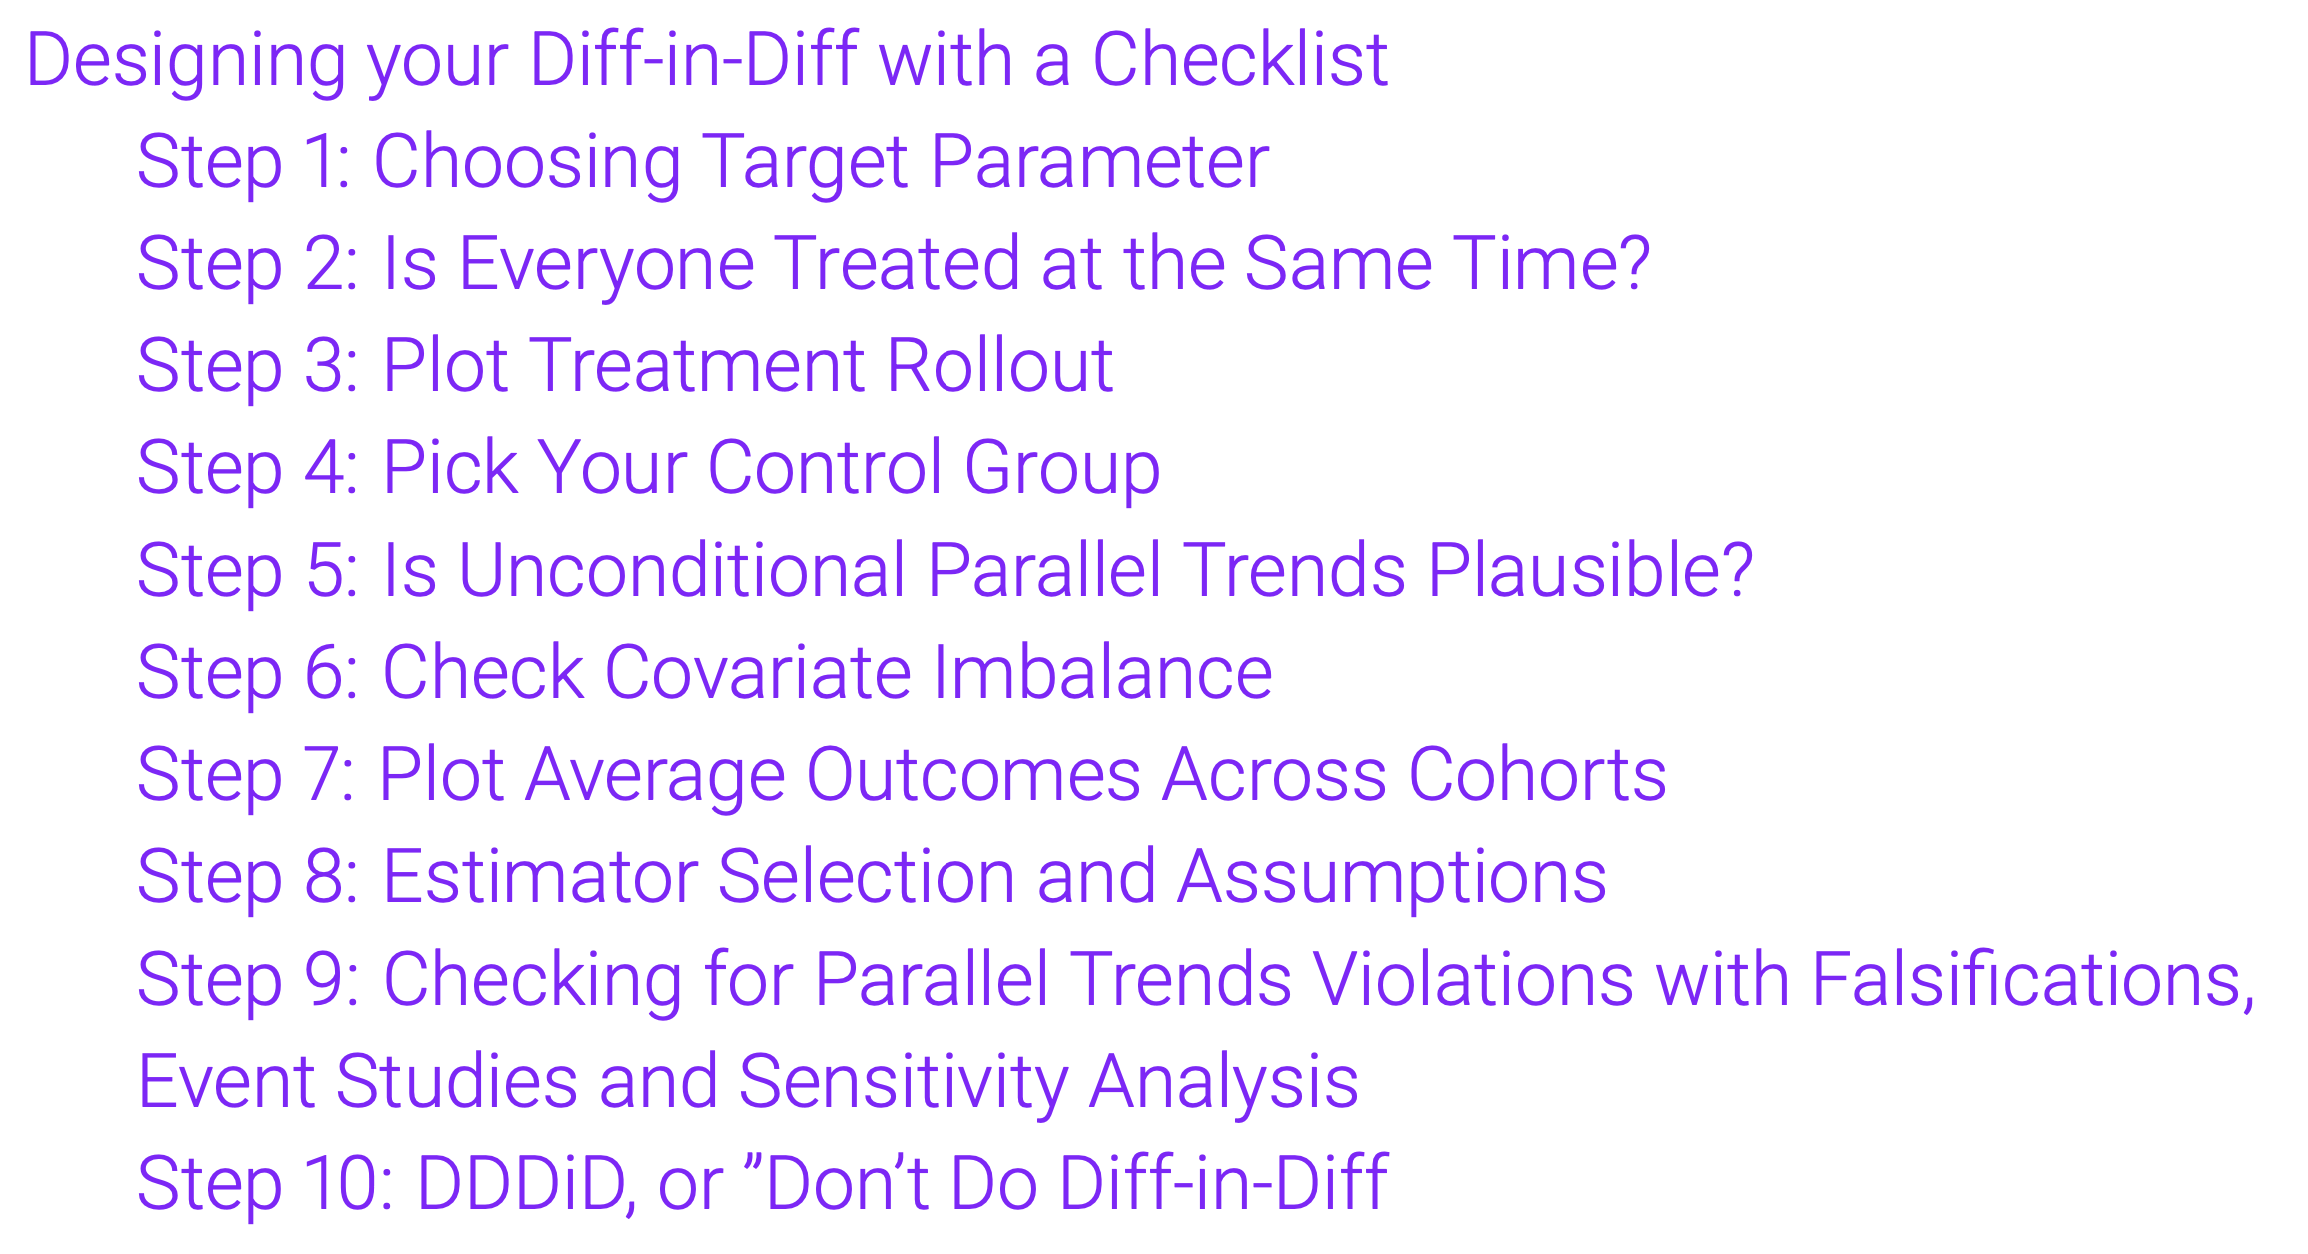
\includegraphics[width=\textwidth]{./lecture_includes/checklist}
\end{figure}

\end{frame}

\begin{frame}{Step 5. Is Unconditional Parallel Trends Plausible?}

\begin{itemize}

\item We have been working with a parallel trends assumption that requires the two \emph{groups} have the same trend in average $Y^0$

\item But what if these two groups were so different from one another that their potential outcomes didn't add up to be the same?

\item What if the workers in the job training program were poor and the control group was rich -- do we think the earnings of those two groups would have been evolved similarly?  Why/why not?



\end{itemize}

\end{frame}


\begin{frame}{You may need a \emph{different} PT assumption}

\begin{itemize}
\item Parallel trends for sub-populations, but not the whole population:
	\begin{enumerate}
	\item Unconditional parallel trends:  parallel trends holds for the overall average treatment and control groups
	\item Conditional parallel trends: parallel trends only has to hold for observable sub-groups, but not necessarily the whole group
	\end{enumerate}
\item Example: Male versus female earnings growth
	\begin{itemize}
	\item Assume male earnings grow by $+2$, female by $+1$, 
	\item Treatment is 75\% male, control is 25\% is male
	\item $E[\Delta Y^0|D=1]=1.75$ but $E[\Delta Y^0|D=0]=1.25$
	\end{itemize}
\item Unconditional parallel trends won't hold because the groups aren't balanced on the characteristics that cause trends 
\end{itemize}

\end{frame}



\begin{frame}{Conditional parallel trends}
Conditional parallel trends (CPT) is a weakened version of the parallel trends assumption requiring that it holds \emph{within} the dimensions of the selected covariates:
\begin{align*}
CPT: \textcolor{red}{E[Y^0_k|Post, X]} - E[Y^0_k|Pre, X] = E[Y^0_U|Post, X] - E[Y^0_U|Pre, X]
\end{align*}
First time it shows up is Heckman, Ichimura and Todd (1997). Idea can be abstract so let's look at a graph to help us decipher what it means and what we can do. And it's still not directly testable due to still missing the first potential outcome (i.e., counterfactual). 
\end{frame}

\begin{frame}{Which covariates do you need?}

\begin{itemize}
\item Conditional parallel trends is tricky because it first assumes you know the covariates you need to satisfy it
\item But how do we decide which variables do this and which ones don't?
\item Econometrics is no help here -- you need common sense, theory, logic, and expertise
\item When selecting covariates, use "confounders" logic -- but confounders of the \emph{trend}?
\end{itemize}

\end{frame}
	



\begin{frame}{Graphs Can Help Pick Covariates}

\begin{figure}[h!]
    \centering
    \begin{tikzpicture}[
        node distance=2.5cm,
        every node/.style={align=center},
        line/.style={->, thick},
    ]
    % Nodes
    \node (X) {Covariates \\ \( X \)};
    \node (D) [below left of=X, xshift=-1cm, yshift=-1cm] {\( D \)};
    \node (DeltaY0) [below right of=X, xshift=1cm, yshift=-1cm] {\( \Delta E\left[Y^0\right] \)};
    % Arrows
    \draw[line] (X) -- (DeltaY0);
    \draw[line] (X) -- (D);
    \end{tikzpicture}
\caption{DAG representing differences in county-level covariate composition (\(X\)) across treatment and control groups (\(D\)) and their determination of the untreated potential outcome trends (\(\Delta E\left[Y^0\right]\)).}
\end{figure}

\end{frame}



\begin{frame}{Example: Concealed Carry Gun Laws and Murder}

\begin{itemize}
\item Become an expert on your left-hand-side variable because you need to know $X \rightarrow \Delta Y^0$
	\begin{itemize}
	\item Drugs and gangs (i.e., crack cocaine epidemic)
	\item Cities had different homicide rates than rural counties
	\item Police, incarceration
	\item Demographics (e.g., race shares, age shares) and economic things (e.g., poverty, per capital income, AFDC rolls)
	\item Maybe throw it all into LASSO using only the $Y^0$ values (maybe pre-treatment murders)
	\end{itemize}
\end{itemize}

\end{frame}



\begin{frame}
 
\begin{figure}
    \centering
    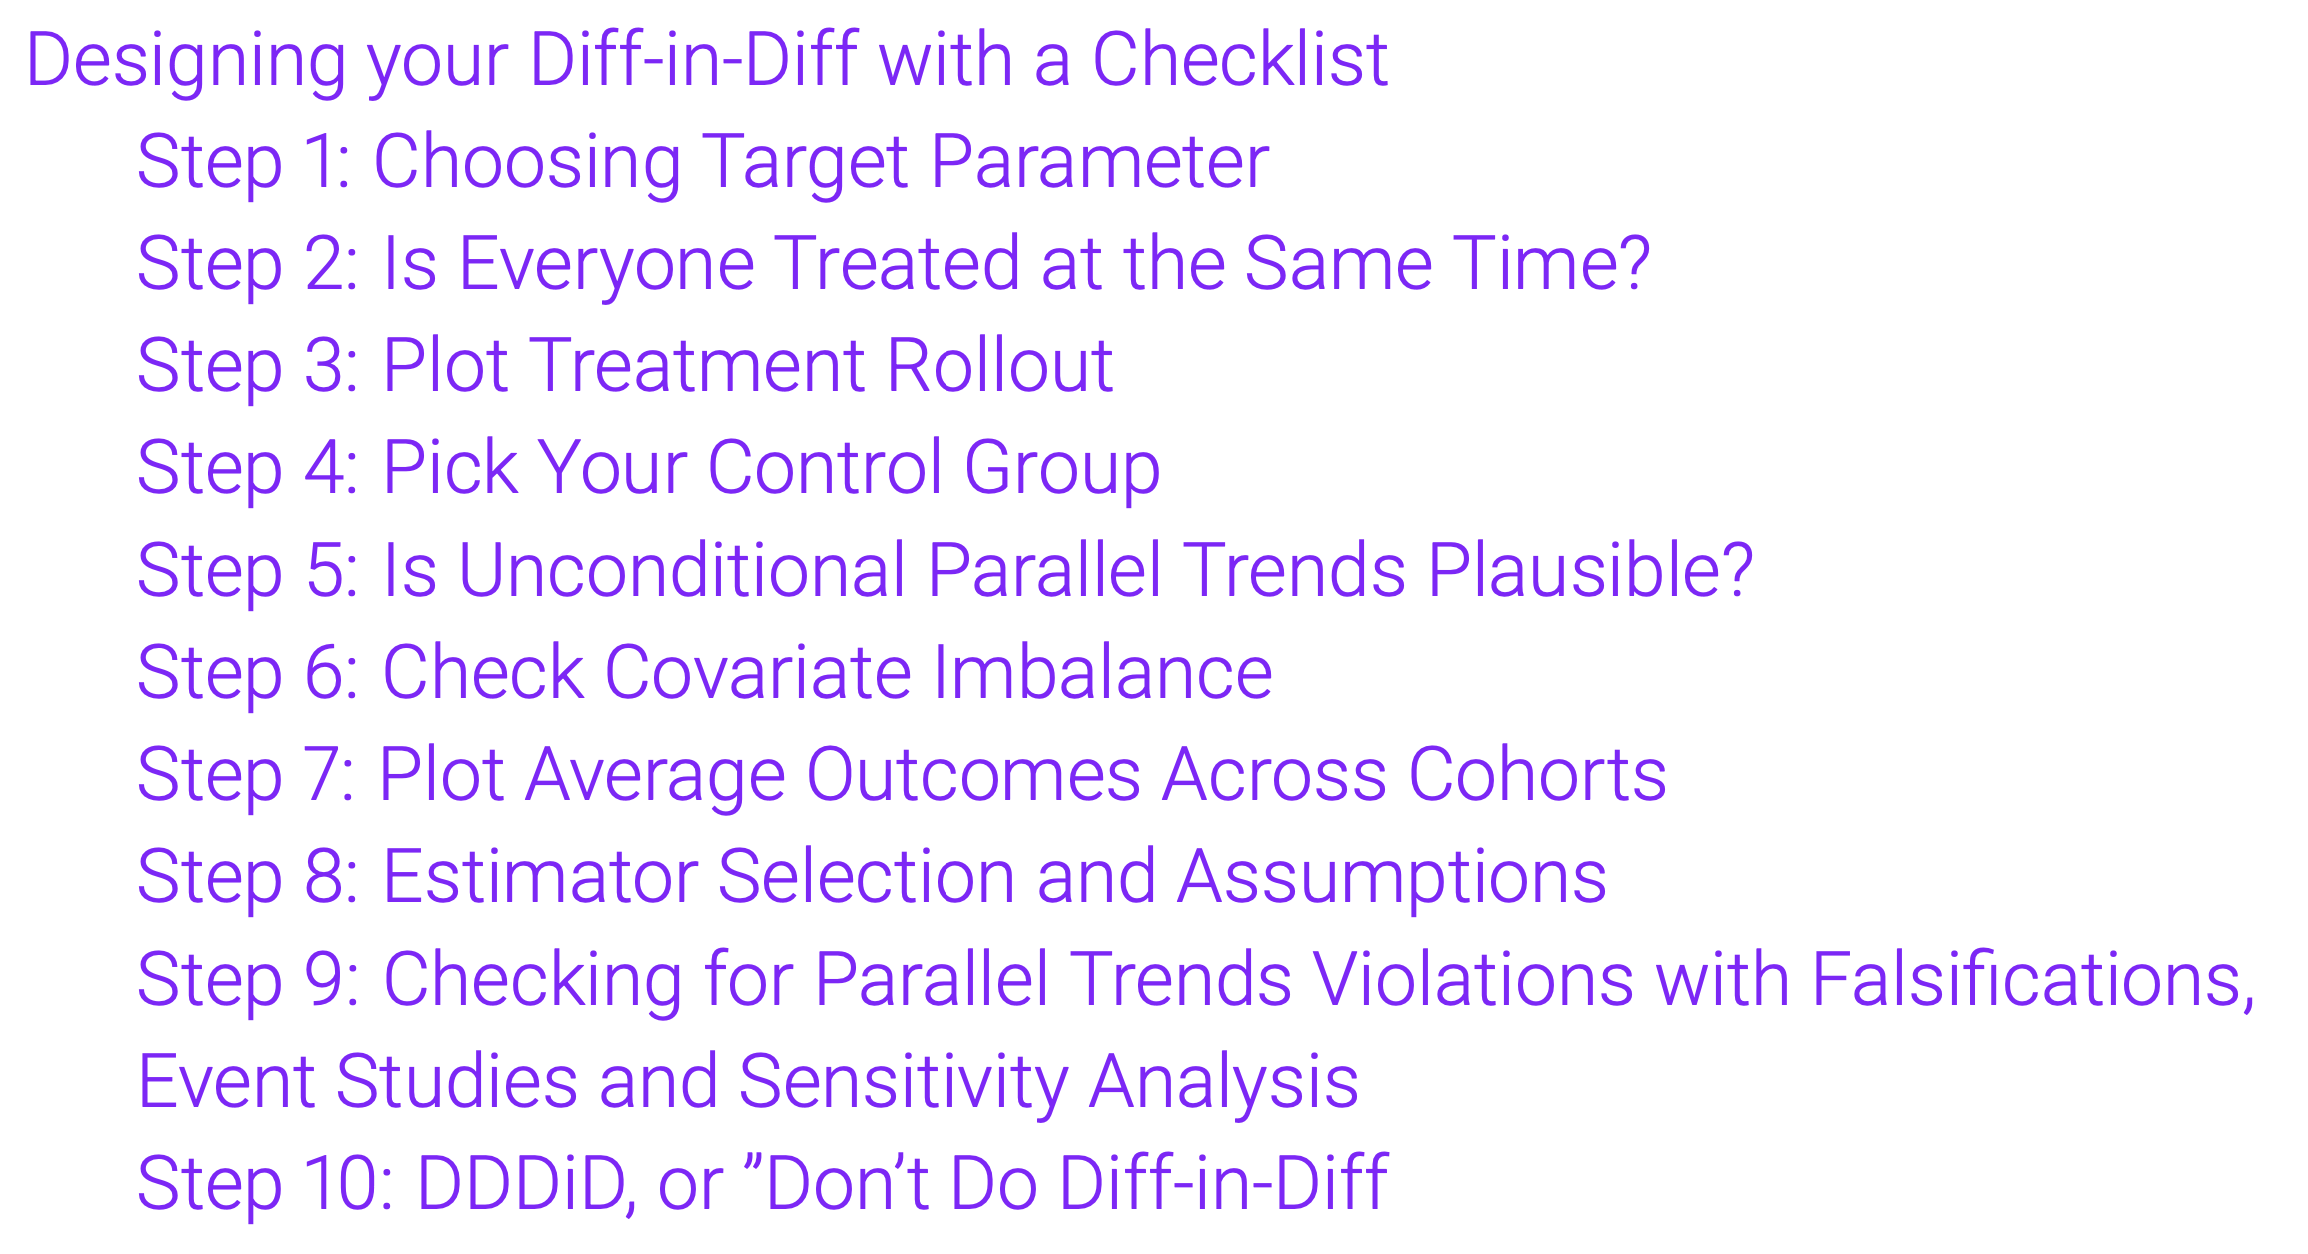
\includegraphics[width=\textwidth]{./lecture_includes/checklist}
\end{figure}

\end{frame}

\begin{frame}{Step 6. Covariate Imbalance}
    \begin{itemize}
	\item Kahn-Lang and Lang (2020) say that if your two groups are different at baseline on outcomes, treatment was not random, is likely caused by covariates, and you need to explain why that matters or does not
	\item Randomized treatment will balance covariates, hence why we don't need to include them as controls in RCT \emph{even though they cause the outcome}
	\item But if they aren't balanced in your diff-in-diff, and they cause \emph{trends}, then parallel trends won't hold
\item So, next you focus on $X \rightarrow D$, which is to say, check the imbalance in covariates you need for conditional parallel trends
\end{itemize}
\end{frame}



\begin{frame}{Create a balance table}

\begin{figure}
    \centering
    \includegraphics[height=0.80\textheight]{./lecture_includes/step6_imbalance}
\end{figure}

\end{frame}


\begin{frame}
    \frametitle{Baseline Covariates and Normalized Difference}
    \begin{itemize}
        \item Baseline covariates are measured before treatment ($t-1$). 
        \item Report the averages of covariates for both groups in a table and the "normalized difference in means" calculated as:
        $$ \text{Norm. Diff}_\omega = \frac{\overline{X}_{\omega,T} - \overline{X}_{\omega,C}}{\sqrt{(S_{\omega,T}^2 + S_{\omega,C}^2)/2}} $$
        \item The normalized difference measures imbalance; it should be less than 0.25 in absolute value to avoid problematic imbalance (Imbens and Rubin 2015).
    \end{itemize}
\end{frame}


\begin{frame}
    \frametitle{Summarizing}
    \begin{itemize}
    \item So, when choosing covariates, remember that there are two steps involved
    	\begin{enumerate}
	\item $X \rightarrow \Delta E[Y^0]$. Pick covariates that are needed to satisfying conditional parallel trends 
	\item $X \rightarrow D$. Check for imbalance using the normalized difference in means equation to determine if you have "problematic imbalance"
	\end{enumerate}
\item And the heuristic I am suggesting is to select covariates that are the "ordinary determinants of $Y^0$" (i.e., become an expert on your left-hand-side variable)
    \end{itemize}
\end{frame}

\begin{frame}
 
\begin{figure}
    \centering
    \includegraphics[width=\textwidth]{./lecture_includes/checklist}
\end{figure}

\end{frame}





\begin{frame}{Step 7: Plot Average Outcomes Across Cohorts}

\begin{itemize}
\item We are literally \textbf{seven} steps into the checklist and this is the first time we are looking at the outcomes (except for baseline)
\item You want to avoid "peeking" at the outcome because you're not wanting to bias yourself and you want this to mimic the RCT as best as you can
\item This is another reason I get frustrated with TWFE -- you can't separate the design from the estimation because the left-hand-side and right-hand-side are both there 
\item Plot the evolution of the mean homicides over time \emph{for each cohort}
\end{itemize}

\end{frame}

\begin{frame}

\begin{figure}
    \centering
    \includegraphics[height=0.85\textheight]{./lecture_includes/step7_outcomes}
\end{figure}

\end{frame}





\subsection{Four Estimators for Covariates}

\begin{frame}
 
\begin{figure}
    \centering
    \includegraphics[width=\textwidth]{./lecture_includes/checklist}
\end{figure}

\end{frame}



\begin{frame}{Step 8. Estimators for Covariates}

\begin{itemize}

\item But, let's say that we feel we have to assume conditional parallel trends
\item What estimators can accomodate that assumption with the least amount of assumptions?
\item We will review four now:
	\begin{enumerate}
	\item Inverse probability weighting
	\item Outcome regression
	\item Double robust
	\item Regressions
	\end{enumerate}
\end{itemize}

\end{frame}


\begin{frame}{Three key covariate estimators in diff-in-diff}

Three papers (though sometimes you see others) about covariate adjustment in DiD:
\begin{enumerate}
\item Abadie (2005) on semiparametric DiD -- reweights the comparison group part of the DID equation using a propensity score based on X
\item Heckman, Ichimura and Todd (1997) on outcome regression uses baseline X and control group only to impute the missing counterfactual $Y^0$ for treatment group units in a DiD equation
\item Sant'Anna and Zhao (2020) is double robust which means the method does both of these at the same time so that you don't have to choose between them
\end{enumerate}

\bigskip

We will discuss both of them and then compare their performance with the more straightforward fixed effects model

\end{frame}






\begin{frame}{Inverse probability weighting}


 Abadie (2005) proposed a model that simply reweights the control group in the DiD equation using a particular specification (``semiparametric'') of the propensity score on pretreatment covariates
 
	\begin{enumerate}
	\item Calculate each unit's ``after minus before'' (DiD equation)
	\item Estimate the conditional probability of treatment based on baseline covariates (propensity score estimation)
	\item Weight the comparison group's DiD equation with the propensity score 
	\end{enumerate}

Remember -- ATT is only missing $Y^0$ for treatment, so we only have to apply weights to the comparison group units

\end{frame}

\begin{frame}{Novel elements of time in Abadie's model}

\begin{itemize}
\item There is only one treatment group so therefore there is only one relevant treatment date, $t$
\item The period prior to treatment is called the baseline, or $b$, period and it is when treated units were not treated 
\item $X_b$ are ``baseline'' covariates meaning the value of $X$ in the pre-treatment period for either the treated or comparison group units
\item Propensity scores are estimated off the $b$ period \emph{only} 
\item Abadie ``throws away'' covariates after treatment because this is all about re-establishing parallel trends which is a \emph{baseline} concept recall
\end{itemize}

\end{frame}

\begin{frame}{Assumptions}

Five main assumptions

\begin{enumerate}
\item No anticipation 
\item SUTVA (no spillovers)
\item Conditional parallel trends $$E[Y^0_t - Y^0_b|D=1,X_b] = E[Y^0_t - Y^0_b | D=0, X_b]$$ 
\item Common support $$Pr(D=1)>0; Pr(D=1|X)<1$$ 
\item Propensity score model is properly specified 
\end{enumerate}

\end{frame}

\begin{frame}{Propensity scores as dimension reduction}

\begin{itemize}

\item Propensity scores are ways of dealing with a conditioning set $X$ that has large dimensions
\item Dimensions are not the same as covariates -- if you have continuous $X$, then it has infinite dimensions
\item Common support means that \emph{within} all combinations of the covariates (e.g., white male 47yo versus whites, males, age) there are units in treatment and control

\end{itemize}

\end{frame}

\begin{frame}{Common support example}

Think of common support like ``exact matches'' but on the propensity score

\bigskip

I'm a white male 47 years old with a PhD; can I find a white male 47 years old without a PhD

\bigskip

If I can, that's common support; if I cannot that's off support

\end{frame}


\begin{frame}{Propensity scores as dimension reduction}

\begin{itemize}

\item Propensity score theorem (Rosenbaum and Rubin 1983) showed that if you need $X$ to satisfy some assumption, the propensity score will satisfy too
\item Propensity scores essentially transform your large dimensional problem into a single scalar called the propensity score, which is the conditional probability of treatment (conditional on $X$)
\item But we need to estimate the propensity score because we don't usually know it (only an experimentalist ``knows'' the true propensity score)

\end{itemize}

\end{frame}

\begin{frame}{Common support and the propensity score}

\begin{itemize}
\item Exact matches mean you have people who are identical on covariate values in both treatment and control
\item Common support and the propensity score means you have people nearly identical on their probability of treatment
\item I am 47yo white male with a PhD with a propensity score of 0.75, but you are an Asian female 27yo without a PhD and have a propensity score of 0.75
\item Same idea, but for this to work, we need to have ``matches'' like that (just on the propensity score)
\end{itemize}

\end{frame}


\begin{frame}{How do these work together?}

Since we are identifying the ATT, and the ATT is missing $Y^0$ for the treated group, we are using the control group $Y^0$ in its place 

\bigskip

Under conditional parallel trends and common support, some of the comparison group units are recovering the parallel trends because of their $X$ values creating projections that in their differences perfectly aligned in expectation with the missing $\Delta E[Y^0|D=1]$

\bigskip

But we have to have all three for it to work

\end{frame}

\begin{frame}{Visualizing propensity score to get common support}

	\begin{figure}
	\includegraphics[scale=0.05]{./lecture_includes/common_support_abadie.png}
	\end{figure}

\end{frame}

\begin{frame}{Definition and estimation}

Defining the ATT parameter of interest
\begin{eqnarray*}
ATT &=& E[Y^1_t - \textcolor{red}{Y^0_t} |D=1] \\
&=&E[Y^1_t  | D = 1 ] - \textcolor{red}{E[Y^0_t | D=1]}
\end{eqnarray*}

\bigskip
Abadie's inverse probability weighting (IPW) estimator
\begin{eqnarray*}
E\bigg [ \frac{Y_t - Y_b}{Pr(D=1)} \times \frac{D - Pr(D=1|X_b)}{1-Pr(D=1|X_b)} \bigg ]
\end{eqnarray*}

\bigskip

The first is our causal parameter; the second is our reweighted DiD equation that \emph{estimates} our causal parameter, but we need to estimate that propensity score


\end{frame}

\begin{frame}{Abadie's IPW estimator}

Look closely; what happens mathematically when you substitute $D=1$ vs $D=0$?

\begin{eqnarray*}
E\bigg [ \frac{Y_t - Y_b}{Pr(D_t=1)} \times \frac{D_t - Pr(D=1|X_b)}{1-Pr(D=1|X_b)} \bigg ]
\end{eqnarray*}

\bigskip

The reweighting with the propensity only happens to the comparison group's first differences -- not the treatment groups!  Why?  Because it's the $Y^0$ that is missing, not the $Y^1$

\end{frame}



\begin{frame}{Propensity scores}

\begin{itemize}
\item It's common to hear people say that we don't know the propensity score; we can only estimate it. Same here -- we approximate it with regressions
\item Paper is titled ``Semi-parametric DiD'' because Abadie imposes structure on the polynomials used to construct the propensity score (``series logit'')
\end{itemize}

\end{frame}







\begin{frame}{Doubly Robust Difference-in-differences}

\begin{itemize}
\item DR models control for covariates twice -- once using the propensity score, once using outcomes adjusted by regression -- and are unbiased so long as:
	\begin{itemize}
	\item The regression specification for the outcome is correctly specified
	\item The propensity score specification is correctly specified
	\end{itemize}
\item Sant'Anna and Zhao (2020) incorporated DR into DiD by combining inverse probability weighting and outcome regression into a single DiD model
\item It's in the engine of Callaway and Sant'Anna (2020) that we discuss later so it merits close study
\end{itemize}

\end{frame}




\begin{frame}{Identification assumptions I: Data}

Assumption 1: Assume panel data or repeated cross-sectional data

\bigskip

Handling repeated cross-sectional data is possible but assumes stationarity which is a kind of stability assumption, but I'll use panel representation. 

\bigskip

Cross-sections will be potentially violated with changing sample compositions (e.g., the Napster example). 

\end{frame}

\begin{frame}{Identification assumptions II: Modification to parallel trends}

Assumption 2: Conditional parallel trends

\bigskip

Counterfactual trends for the treatment group are the same as the control group for all values of $X$

\begin{eqnarray*}
E[Y_1^0 - Y_0^0 | X, D=1] = E[Y^0_1 - Y^0_0 | X, D=0]
\end{eqnarray*}

\end{frame}

\begin{frame}{Identification assumptions III: Common support}

Assumption 3: Common support

\bigskip

For some $e>0$, the probability of being in the treatment group is greater than $e$ and the probability of being in the treatment group conditional on $X$ is $\leq1-e$. 

\bigskip

Heckman, et al doesn't use the propensity score so we need a more general expression of support

\end{frame}

\begin{frame}{Estimating DD with Assumptions 1-3}

\begin{itemize}
\item Assumptions 1-3 gives us a couple of options of estimating the DiD
\item We can either use the outcome regression (OR) approach of Heckman, et al 1997 (will require correct model too)
\item Or we can use the inverse probability weighting (IPW) approach of Abadie (2005) (will require correct model too)
\end{itemize}

\end{frame}



\begin{frame}{Outcome regression}

This is the Heckman, et al. (1997) approach where the potential outcome evolution for the treatment group is imputed with a regression based only on $X_b$ for the control group \emph{only}

\bigskip

\begin{eqnarray*}
\widehat{\delta}^{OR} = \bigg [ \overline{Y}_{1,1} -  \overline{Y}_{1,0} \bigg ] -  \bigg [ \frac{1}{n^T} \sum_{i|D_i=1} ( \widehat{\mu}_{0,1}(X_i) - \widehat{\mu}_{0,0}(X_i)) \bigg ]
\end{eqnarray*}

where $\overline{Y}$ is the sample average of $Y$ among units in the treatment group at time $t$ and $\widehat{\mu}(X)$ is an estimator of the true, but unknown, $m_{d,t}(X)$ which is by definition equal to $E[Y_t|D=d,X=x]$.

\end{frame}




\begin{frame}{Outcome regression}

\begin{eqnarray*}
\widehat{\delta}^{OR} = \bigg [ \overline{Y}_{1,1} -  \overline{Y}_{1,0} \bigg ] -  \bigg [ \frac{1}{n^T} \sum_{i|D_i=1} ( \widehat{\mu}_{0,1}(X_i) - \widehat{\mu}_{0,0}(X_i)) \bigg ]
\end{eqnarray*}

\begin{enumerate}
\item Regress changes $\Delta Y$ on $X$ among untreated groups using baseline covariates only
\item Get fitted values of the regression using all $X$ from $D=1$ only.  Average those
\item Calculate change in this fitted $Y$ among treated with the average fitted values
\end{enumerate}

\end{frame}

\begin{frame}{Inverse probability weighting}

This is the Abadie (2005) approach where we use weighting

\begin{eqnarray*}
\widehat{\delta}^{ipw} = \frac{1}{E_N[D]} E \bigg [ \frac{D-\widehat{p}(X)}{1-\widehat{p}(X)} (Y_1-Y_0) \bigg ]
\end{eqnarray*}

where $\widehat{p}(X)$ is an estimator for the true propensity score. Reduces the dimensionality of $X$ into a single scalar.

\end{frame}

\begin{frame}{These models cannot be ranked}

\begin{itemize}
\item Outcome regression needs $\widehat{\mu}(X)$ to be correctly specified, whereas
\item Inverse probability weighting needs $\widehat{p}(X)$ to be correctly specified
\item It's hard to ``rank'' these two in practice with regards to model misspecification because each is inconsistent when their own models are misspecified
\item But what if you could do both of them at the same time and not pay for it?
\end{itemize}

\end{frame}

\begin{frame}{Double Robust DR}

\begin{itemize}
\item Doubly robust combines them to give us insurance; we now get two chances to be wrong, as opposed to just one
\item Two papers:
	\begin{enumerate}
	\item Chang (2020) incorporates DR with double/debiased ML
	\item Sant'Anna and Zhao (2020) is based on the IPW (Abadie 2005) and OR (Heckman, Ichimura and Todd 1997)
	\end{enumerate}
\item For now, I've prepped the latter, but will soon get Chang (2020) incorporated -- I just have been relying on Brigham Frandsen to teach the DML material
\end{itemize}

\end{frame}



\begin{frame}{Double Robust DiD}
\begin{eqnarray*}
\delta^{dr} = E \bigg [ \bigg ( \frac{D}{E[D]} -\frac{ \frac{p(X)(1-D)}{(1-p(X))} }{E \bigg [\frac{p(X)(1-D)}{(1-p(X))} \bigg ]} \bigg  )( \Delta Y - \mu_{0,\Delta}(X)) \bigg ]
\end{eqnarray*}

\begin{eqnarray*}
&&p(x): \text{propensity score model} \\
&& \Delta Y = Y_1 - Y_0 = Y_{post} - Y_{pre} \\
&& \mu_{d,\Delta} = \mu_{d,1}(X) - \mu_{d,0}(X), \text{ where } \mu(X) \text{ is a model for} \\
&& m_{d,t} = E[Y_t|D=d,X=x]
\end{eqnarray*}So that means $\mu_{0,\Delta}$ is just the control group's change in average $Y$ for each $X=x$

\end{frame}

\begin{frame}{Double Robust DiD}

\begin{eqnarray*}
\delta^{dr} = E \bigg [ \bigg ( \frac{D}{E[D]} -\frac{ \frac{p(X)(1-D)}{(1-p(X))} }{E \bigg [\frac{p(X)(1-D)}{(1-p(X))} \bigg ]} \bigg  )( \Delta Y - \mu_{0,\Delta}(X)) \bigg ]
\end{eqnarray*}

Notice how the model controls for $X$: you're weighting the adjusted outcomes using the propensity score

\bigskip

The reason you control for $X$ twice is because you don't know which model is right.  DR DiD frees you from making a choice without making you pay too much for it


\end{frame}

\begin{frame}{Efficiency}

\begin{itemize}
\item Authors exploit all the restrictions implied by the assumptions to construct semiparametric bounds
\item This is where the influence function comes in, which those who have studied the DID code closely may have noticed
\item One of the main results of the paper is that the DR DiD estimator is also DR for inference
\end{itemize}

\end{frame}


\begin{frame}{Standard TWFE Model}

Consider our earlier TWFE specification:

\begin{eqnarray*}
Y_{it} = \alpha_1  + \alpha_2 T_t + \alpha_3 D_i +  \delta (T_i \times D_t)  + \varepsilon_{it}
\end{eqnarray*}

\bigskip

Just add in covariates then right?

\begin{eqnarray*}
Y_{it} = \alpha_1  + \alpha_2 T_t + \alpha_3 D_i  + \delta (T_i \times D_t) + \theta \cdot X_{it} + \varepsilon_{it}
\end{eqnarray*}

Sure! If you're willing to impose three \emph{more} assumptions

\end{frame}




\begin{frame}{Decomposing TWFE with covariates}

TWFE places restrictions on the DGP. Previous TWFE regression under assumptions 1-3 implies the following:

\bigskip

\begin{eqnarray*}
E[Y^1_1|D=1,X] = \alpha_1 + \alpha_2 + \alpha_3 + \delta + \theta X
\end{eqnarray*}

\bigskip

Conditional parallel trends implies

\small
\begin{eqnarray*}
&&E[Y^0_{1} - Y^0_{0}|D=1,X]= E[Y^0_{1} - Y^0_{0}|D=0,X] \\
&&E[Y^0_{1}|D=1,X] - E[Y^0_{0}|D=1,X]= E[Y^0_{1}|D=0,X] - E[Y^0_{0}|D=0,X] \\
&&E[Y^0_{1}|D=1,X] = E[Y^0_{0}|D=1,X] + E[Y^0_{1}|D=0,X] - E[Y^0_{0}|D=0,X] \\
&&E[Y^0_{1}|D=1,X] = E[Y_{0}|D=1,X] + E[Y_{1}|D=0,X] - E[Y_{0}|D=0,X] \\
\end{eqnarray*}


\end{frame}

\begin{frame}{Switching equation substitution}

Last line from the switching equation. This gives us:

\begin{eqnarray*}
E[Y^0_{1}|D=1,X] = \alpha_1  + \alpha_2 + \alpha_3 + \theta X
\end{eqnarray*}

Now compare this with our earlier $Y^1$ expression

\begin{eqnarray*}
E[Y^1_1|D=1,X] = \alpha_1 + \alpha_2 + \alpha_3 + \delta + \theta X
\end{eqnarray*}

We can define our target parameter, the ATT, now in terms of the fixed effects representation

\end{frame}


\begin{frame}{Collecting terms}

TWFE representation of our conditional expectations of the potential outcomes
\begin{eqnarray*}
&&E[Y^1_1|D=1,X] = \alpha_1 + \alpha_2 + \alpha_3 + \delta + \theta_1 X \\
&&E[Y^0_{1}|D=1,X] = \alpha_1  + \alpha_2 + \alpha_3 + \theta_2 X \\
\end{eqnarray*}

Substitute these into our target parameter

\begin{eqnarray*}
ATT &=& E[Y^1_1|D=1,X]  - E[Y^0_{1}|D=1,X]   \\
&&=(\alpha_1 + \alpha_2 + \alpha_3 + \delta + \theta_1 X) - ( \alpha_1  + \alpha_2 + \alpha_3 + \theta_2 X )\\
&&=\delta + (\theta_1 X - \theta_2 X)
\end{eqnarray*}

\bigskip

What if $\theta_1 X \neq \theta_2 X$?

\end{frame}

\begin{frame}{Assumption 4: Homogeneous treatment effects in X}


TWFE requires homogenous treatment effects in $X$ (i.e., the treatment effect is the same for all $X$)

\bigskip

If $X$ is sex, then effects are the same for males and females.

\bigskip

  If $X$ is continuous, like income, then the effect is the same whether someone makes \$1 or \$1 million.

\end{frame}

\begin{frame}{X-specific trends}

TWFE also places restrictions on covariate trends for the two groups too.  Take conditional expectations of our TWFE equation. 

\begin{eqnarray*}
E[Y_1|D=1] &=& \alpha_1 + \alpha_2 + \alpha_3 + \delta + \theta X_{11} \\
E[Y_0|D=1] &=& \alpha_1 + \alpha_3 + \theta X_{10} \\
E[Y_1|D=0] &=& \alpha_1 + \alpha_2 + \theta X_{01} \\
E[Y_0|D=0] &=& \alpha_1 + \theta X_{00}
\end{eqnarray*}


\end{frame}


\begin{frame}{X-specific trends}

Now take the DiD formula:

\begin{eqnarray*}
\delta^{DD} = &&\bigg ( (\alpha_1 + \alpha_2 + \alpha_3 + \delta + \theta X_{11} ) - (\alpha_1 + \alpha_3 + \theta X_{10} ) \bigg )- \\
&& \bigg ( (\alpha_1 + \alpha_2 + \theta X_{01}) - (\alpha_1 + \theta X_{00}) \bigg )
\end{eqnarray*}

\bigskip

Eliminating terms, we get:

\begin{eqnarray*}
\delta^{DD} = &&\delta + \\
&& (\theta X_{11} - \theta X_{10} ) - (\theta X_{01} - \theta X_{00} )
\end{eqnarray*}

\bigskip

Second line requires that trends in X for treatment group equal trends in X for control group.

\end{frame}


\begin{frame}{Assumption 5 and 6}

We need ``no X-specific trends'' for the treatment group (assumption 5) and comparison group (assumption 6)

\bigskip

\textbf{Intuition}: No X-specific trends means the evolution of potential outcome $Y^0$ is the same regardless of $X$. This would mean you cannot allow rich people to be on a different trend than poor people, for instance.

\bigskip

Without these six, in general TWFE will not identify ATT. 

\end{frame}

\begin{frame}{Why not both?}

\begin{itemize}
\item Let's review the problem.  What if you claim you need $X$ for conditional parallel trends?
\item You have three options:
	\begin{enumerate}
	\item Outcome regression (Heckman, et al. 1997) -- needs Assumptions 1-3
	\item Inverse probability weighting (Abadie 2005) -- needs Assumptions 1-3
	\item TWFE (everybody everywhere all the time) -- needs Assumptions 1-6
	\end{enumerate}
\item Problem is 1 and 2 need the models to be correctly specified
\item Let's look at a couple of Monte Carlos -- one by Pedro Sant'Anna, and then one by me
\end{itemize}

\end{frame}






\begin{frame}{R and Stata Code}

There is code in R and Stata (all DiD estimators are now beautifully arranged at a website hosted by Asjad Naqvi)
\begin{itemize}
\item Stata: \textbf{drdid}
\item R: \textbf{drdid}
\end{itemize}

\bigskip

\url{https://asjadnaqvi.github.io/DiD/docs/01_stata/}

\bigskip

Remember -- it's for 2x2 with covariates (i.e., one treatment group). 

\end{frame}


\begin{frame}{Monte Carlo Simulations}

\begin{itemize}

\item First we will look at the use of these estimators using a simulation named \texttt{covariates.do} and \texttt{covariates.R}

\item We will do it both with a single run, as that's faster, and then run a simulation of 1,000 simulated regenerated data (i.e., Monte Carlo simulation) to get a distribution

\item We will examine all four estimators: (1) OLS, (2) IPW, (3) OR and (4) DR

\end{itemize}

\end{frame}

\begin{frame}{Simulation}
    \centering
    \includegraphics[width=0.6\textwidth]{./lecture_includes/covariates.jpg}
\end{frame}



\begin{frame}{Event studies can mislead}

\begin{itemize}

\item People mistakenly equate parallel trends with parallel pretrends, but you can have one without the other, both or neither
\item One of the ways you can have parallel pre-trends but violate parallel trends is if the trends change differentially by covariate over time (called x-specific trends)
\item Code is called \texttt{misleading_eventstudy.do} and \texttt{misleading_eventstudy.R}
\item Note how well the unconditional parallel trends assumption appears to be when reviewing the graphs only
\end{itemize}

\end{frame}

\begin{frame}{Event studies can mislead}

\begin{figure}
    \centering
    \includegraphics[height=0.75\textheight]{./lecture_includes/es_flawed.png}
\end{figure}

\end{frame}


\begin{frame}{Event studies can mislead}

\begin{figure}
    \centering
    \includegraphics[height=0.75\textheight]{./lecture_includes/es_correct.png}
\end{figure}

\end{frame}

\begin{frame}{Time varying trends in $Y^0$ have \emph{nothing} to do with parallel trends}

\begin{figure}
    \centering
    \includegraphics[height=0.75\textheight]{./lecture_includes/misleading_eventstudy_code}
\end{figure}

\end{frame}

\begin{frame}{Selection can also make event studies misleading}

\begin{itemize}

\item Remember from earlier: some forms of selection that satisfy parallel trends will nonetheless complicate event study plots
\item Selection on baseline $Y^0$, for instance, can cause the pre-trends to break but not parallel trends
\end{itemize}

\end{frame}

\begin{frame}{Selection on $Y^0$ and event studies}

\begin{figure}
    \centering
    \includegraphics[height=0.70\textheight]{./lecture_includes/selection_y0.png}
\end{figure}

\end{frame}










\begin{frame}{What is the event study for?}

\begin{itemize}

\item The purpose of the event study is as a \emph{falsification}, not as a proof of the parallel trends
\item Falsifications should be the \emph{same} model used for estimation but applied to something that it cannot cause -- "same group, different outcome"
\item In this case, future treatments under no anticipation cannot affect the past
\item Since the estimation of post-treatment ATT use $t-1$ for "pre" period, the falsifications in the event studies should too 
\end{itemize}

\end{frame}


\begin{frame}{Short vs Long Difference Calculation}

\begin{itemize}
\item OLS always drops a single $t-1$ baseline year which means event studies are calculated using "long differences"
\item But the newer methods are not regression based, and therefore open the door for two ways to do the calculation
	\begin{enumerate}
	\item \textbf{Long differences}: each event study will be a simple 2x2 using the same baseline as used in the post-treatment calculations
	\item \textbf{Short gaps}: pre-treatment coefficients will be calculated using a "moving" baseline, usually the one right next to it
	\end{enumerate}
\item You can tell this one is using short gaps, for instance, because otherwise how is there a $t-1$ coefficient?
\end{itemize}

\end{frame}


\begin{frame}

\begin{figure}
    \centering
    \includegraphics[height=0.5\textheight]{./lecture_includes/magic_johnson_eventstudy}
\end{figure}

\end{frame}



\begin{frame}{Example}

\begin{itemize}

\item Has become a source of confusion due in part to documentation in some software being vague on this point
\item Appears to be very little awareness of this as you will see it done both ways, but they cannot both be the correct representation as it's possible to reject trends in one but not the other 
\item Let's look at an example from my project
\end{itemize}

\end{frame}

\begin{frame}{Real world example of questionable unconditional parallel trends}

\begin{itemize}
\item Me, Christine Durrance, and Melanie Guldi have been working on a project for years looking at online dating's effect on birth rates
	\begin{itemize}
	\item Thickening of relationship markets
	\item Reduced search costs
	\item Formation of better relationships meant for forming families
	\end{itemize}
\item But online dating companies have an incentive to perpetuate dating despite claims to the contrary, which may reduce the formation of families
\item Plus so many confounders -- websites appeared simultaneously, smart phones, social media, and birth rates plummeted after Great Recession ("demographic transition")
\end{itemize}
\end{frame}





\begin{frame}

\begin{figure}
    \centering
    \includegraphics[height=0.95\textheight]{./lecture_includes/craigslist_online}
\end{figure}

\end{frame}



\begin{frame}

\begin{figure}
    \centering
    \includegraphics[height=0.85\textheight]{./lecture_includes/es_br1544_shortgap.png}
\end{figure}

\end{frame}


\begin{frame}{Scrutinizing that event study}

\begin{itemize}
\item There are two things going on in that graph
	\begin{enumerate}
	\item Notice the decline in coefficients leading into $t-1$ as opposed to $t-1$ being a solid circle -- called "short gap" calculation of event study coefficients, which is possible with new estimators but impossible with regressions
	\item No covariates
	\end{enumerate}
\item We are comparing each period to the period to its left, but OLS used the $t-1$ as its baseline
\item Plus without controlling for covariates, we are assuming that ordinarily, small and large counties would have evolved similarly, but we know sorting into large vs small counties is not random
\end{itemize}
\end{frame}

\begin{frame}{Scrutinizing that event study}

\begin{itemize}
\item So we do two things: 
	\begin{enumerate}
	\item We use the same method as OLS for calculating the event studies ("long difference"), 
	\item We include a control for how urban the county is with a 9-digit variable (RUCC)
	\end{enumerate}
\item Compare the first event study to the last one, and see if you can spot the difference 
\end{itemize}
\end{frame}

\begin{frame}{Short Gap vs. Long Difference}

\begin{figure}[htbp]
    \centering
    \begin{minipage}[b]{0.48\textwidth}
        \centering
        \includegraphics[width=\textwidth,height=0.75\textheight,keepaspectratio]{./lecture_includes/es_br1544_shortgap.png}
        \caption{Short Gap}
    \end{minipage}
    \hfill
    \begin{minipage}[b]{0.48\textwidth}
        \centering
        \includegraphics[width=\textwidth,height=0.75\textheight,keepaspectratio]{./lecture_includes/es_births2.png}
        \caption{Long Difference}
    \end{minipage}
\end{figure}

\pause

\begin{itemize}
\item Question 1: how could you have seen that the event study was "short gap" vs "long difference"? \pause
\item Question 2: What is the relationship between the negative coefficients under short gap and the positive coefficients in long difference?
\end{itemize}

\end{frame}

\begin{frame}{Is Unconditional parallel trends plausible?}

\begin{itemize}
\item Without covariates, we are explicitly assuming that the treatment and control group would have evolved similarly in birth rates
\item But what if Craigslist entered certain kinds of counties differently than others?
\item What if the ones it entered earlier had different birth rate trends?
\item Let's look at the rollout by urban status
\end{itemize}

\end{frame}

\begin{frame}{Small numbers are more urban}

\begin{figure}
    \centering
    \includegraphics[height=0.85\textheight]{./lecture_includes/pretty_RUCC}
\end{figure}

\end{frame}






\begin{frame}

\begin{figure}
    \centering
    \includegraphics[height=0.95\textheight]{./lecture_includes/es_br1544_combined.png}
\end{figure}

\end{frame}

\begin{frame}{Shoeleather and DiD}

\begin{itemize}

\item Do everything you can to understand selection -- shoeleather dominates technical knowledge (Rubin 2008 "Design Trumps Analysis"; Freedman 1991)
\item John Snow did not just download data and run regressions -- he worked hard to find comparable groups, learn the institutional details, and think carefully about selection
\item Do everything you can to figure out the treatment assignment mechanism 
\item Consider interviewing key people!
\end{itemize}

\end{frame}

\begin{frame}[shrink=20]
    \centering
    \begin{center}
    \begin{figure}
        \includegraphics[width=\textwidth]{./lecture_includes/craig_dm}
    \end{figure}
    \end{center}
    
    \vspace{0.5cm} % Add some space between the image and the text

    
\end{frame}



\begin{frame}{What happened?}

\begin{itemize}
\item What happened?  Craigslist tended to target urban counties so treatment were highly urban and control highly rural
\item Remember that what's missing in the ATT is $\textcolor{red}{E[Y^0|D=1]}$ and we use the control group trends in its $Y^0$ to \emph{impute} the missing $\textcolor{red}{E[Y^0|D=1]}$
\item It's actually pretty basic -- do you think cities have different birth rate trends than counties?  If so, then that imputation is likely to be bad
\item But what if you imputed $Y^0$ apples for apples -- use cities in the control to impute cities in the treatment

\end{itemize}
\end{frame}




\begin{frame}{Application using real data}

\begin{itemize}
\item Let's now use a real example with real data and see how well this does
\item Famous paper in AER by Lalonde (1986), an Orley and Card student at Princeton
\item Found that most program evaluation did badly, but let's revisit it with diff-in-diff
\end{itemize}

\end{frame}

\begin{frame}{Description of NSW Job Trainings Program}
	
The National Supported Work Demonstration (NSW), operated by Manpower Demonstration Research Corp in the mid-1970s:
	\begin{itemize}
	\item was a temporary employment program designed to help disadvantaged workers lacking basic job skills move into the labor market by giving them work experience and counseling in a sheltered environment
	\item was also unique in that it \textbf{randomly assigned} qualified applicants to training positions:
		\begin{itemize}
		\item \textbf{Treatment group}: received all the benefits of NSW program
		\item \textbf{Control group}: left to fend for themselves
		\end{itemize}
	\item admitted AFDC females, ex-drug addicts, ex-criminal offenders, and high school dropouts of both sexes
	\end{itemize}
\end{frame}

\begin{frame}{NSW Program}
	
	\begin{itemize}
	\item Treatment group members were:
		\begin{itemize}
		\item guaranteed a job for 9-18 months depending on the target group and site
		\item divided into crews of 3-5 participants who worked together and met frequently with an NSW counselor to discuss grievances and performance
		\item paid for their work
		\end{itemize}
	\item Control group members were randomized so the same
	\item Note: the randomization balanced observables and unobservables across the two arms, thus enabling the estimation of an ATE for the people who self-selected into the program
	\end{itemize}
\end{frame}

\begin{frame}{NSW Program}

\begin{itemize}
	\item Other details about the NSW program:
		\begin{itemize}
		\item \underline{Wages}:  NSW offered the trainees lower wage rates than they would've received on a regular job, but allowed their earnings to increase for satisfactory performance and attendance
		\item \underline{Post-treatment}: after their term expired, they were forced to find regular employment
		\item \underline{Job types}:  varied within sites -- gas station attendant, working at a printer shop -- and males and females were frequently performing different kinds of work
		\end{itemize}
\end{itemize}

\end{frame}
	
\begin{frame}{NSW Data}
	
	\begin{itemize}
	\item \underline{NSW data collection}:
		\begin{itemize}
		\item MDRC collected earnings and demographic information from both treatment and control at baseline and every 9 months thereafter
		\item Conducted up to 4 post-baseline interviews
		\item Different sample sizes from study to study can be confusing, but has simple explanations
		\end{itemize}
	\end{itemize}
\end{frame}
	

\begin{frame}{NSW Data}

\begin{itemize}
	\item \underline{Estimation}:
		\begin{itemize}
		\item NSW was a randomized job trainings program; therefore estimating the average treatment effect is straightforward:
			\begin{eqnarray*}
			\frac{1}{N_t}\sum_{D_i=1}Y_i - \frac{1}{N_c}\sum_{D_i=0}Y_i \approx E[Y^1-Y^0] 
			\end{eqnarray*}in large samples assuming treatment selection is independent of potential outcomes (randomization) -- i.e., $(Y^0,Y^1)\independent{D}$. 
		\end{itemize}
	\item \underline{NSW worked}: Treatment group participants' real earnings post-treatment (1978) was positive and economically meaningful -- $\approx$ \$900 (LaLonde 1986) to \$1,800 (Dehejia and Wahba 2002) depending on the sample used
\end{itemize}

\end{frame}
	
\begin{frame}[plain]
	\begin{center}
	LaLonde, Robert J. (1986). \myurlshort{http://business.baylor.edu/scott_cunningham/teaching/lalonde-1986.pdf}{``Evaluating the Econometric Evaluations of Training Programs with Experimental Data''}. \emph{American Economic Review}. 
	\end{center}
	
\underline{LaLonde's study} was \textbf{not} an evaluation of the NSW program, as that had been done, but rather an evaluation of econometric models done by:
		\begin{itemize}
		\item replacing the experimental NSW control group with non-experimental control group drawn from two nationally representative survey datasets: Current Population Survey (CPS) and Panel Study of Income Dynamics (PSID)
		\item estimating the average effect using non-experimental workers as controls for the NSW trainees 
		\item comparing his non-experimental estimates to the experimental estimates of \$900
		\end{itemize}
\end{frame}

\begin{frame}{LaLonde (1986)}

\begin{itemize}

	\item \underline{LaLonde's conclusion}: available econometric approaches were biased and inconsistent
		\begin{itemize}
		\item His estimates were way off and usually the wrong sign
		\item Conclusion was influential in policy circles and led to greater push for more experimental evaluations
		\end{itemize}

\end{itemize}

\end{frame}

\imageframe{./lecture_includes/lalonde_table5a.png}
\imageframe{./lecture_includes/lalonde_table5b.png}

\begin{frame}[plain,shrink=10]{Imbalanced covariates for experimental and non-experimental samples}

    \begin{center}
		\begin{table}
		\begin{tabular}{lcccccc}
		\hline \hline
		\multicolumn{3}{c}{}&
		\multicolumn{1}{c}{CPS}&
		\multicolumn{1}{c}{NSW}\\
		
		\multicolumn{1}{c}{}&
		\multicolumn{2}{c}{All} &
		\multicolumn{1}{c}{Controls} &
		\multicolumn{1}{c}{Trainees} \\

		\multicolumn{3}{c}{}&
		\multicolumn{1}{c}{$N_c=15,992$}&
		\multicolumn{1}{c}{$N_t=297$}&
		\multicolumn{1}{c}{}&
		\multicolumn{1}{c}{}\\

		\multicolumn{1}{l}{covariate}&
		\multicolumn{1}{c}{mean}&
		\multicolumn{1}{c}{(s.d.)}&
		\multicolumn{1}{c}{mean}&
		\multicolumn{1}{c}{mean}&
		\multicolumn{1}{c}{t-stat}&
		\multicolumn{1}{c}{diff}\\
		\hline
Black    & 0.09 & 0.28 & 0.07 & 0.80 & 47.04 & -0.73\\
Hispanic & 0.07 & 0.26 & 0.07 & 0.94 & 1.47 & -0.02\\
Age & 33.07 & 11.04 & 33.2 & 24.63 & 13.37  & 8.6\\
Married & 0.70 & 0.46 & 0.71 & 0.17 & 20.54 & 0.54\\
No degree & 0.30 & 0.46 & 0.30 & 0.73 & 16.27 & -0.43\\
Education & 12.0 & 2.86 & 12.03 & 10.38 & 9.85 & 1.65 \\
1975 Earnings   & 13.51 & 9.31 & 13.65 & 3.1 & 19.63 & 10.6\\
1975 Unemp  & 0.11 & 0.32 & 0.11 & 0.37 & 14.29 & -0.26\\
		\hline 
		\end{tabular}
		\end{table}
    \end{center}

\end{frame}


\begin{frame}{Lab}

\url{https://github.com/Mixtape-Sessions/Causal-Inference-2/tree/main/Lab/Lalonde}

\bigskip

Together let's do questions 1 and 2a-c

\end{frame}




\begin{frame}{Concluding remarks}

\begin{itemize}
\item Including covariates in a DiD design is done for reasons that are different than in regressions more generally -- we are trying to address a parallel trends violation
\item Typical regression modeling can only incorporate covariates, but that places restrictions on the model, whereas other methods will not
\item We use baseline covariates because we cannot include covariates that are outcomes otherwise it introduces its own biases
\item Doubly robust and IPW incorporate covariates through propensity scores and outcome regressions (or both) using baseline covariate means only
\end{itemize}

\end{frame}

\begin{frame}{Suggestions}

\begin{itemize}

\item Remember that the threat to validity comes from comparing aggregate groups of units for whom differences in observables, with different associations with $Y^0$, violate parallel trends
\item Conditional parallel trends simply requires that groups which are comparable on covariates are more likely to have comparable $Y^0$ trends
\item Check for imbalance at baseline using normalized differences
\item Choose covariates that are highly predictive of the missing potential outcome, $Y^0$

\end{itemize}

\end{frame}



\subsection{Estimators for differential timing} 

\begin{frame}{Step 8: Estimator Selection for Differential Timing}

\begin{itemize}
\item What if there had not been just one treatment cohort, but several? 
\item Think of there being three options with differential timing 
	\begin{enumerate}
	\item Traditional twoway fixed effects (TWFE)
	\item Aggregating ATT(g,t) using Callaway and Sant'Anna or Sun and Abraham
	\item Imputation using Borusyak, Jaravel and Speiss, Gardner or Wooldridge
	\end{enumerate}
\item  Let's review now the differential timing literature with an aim to making a decision among them
\end{itemize}

\end{frame}

\begin{frame}{Five approaches we will study}

\begin{enumerate}
\item Twoway fixed effects (Goodman-Bacon 2021)
\item Callaway and Sant'Anna (2021), or CS
\item Sun and Abraham (2021), or SA
\item de Chaisemartin and D'Haultfouielle (2020), or dCDH
\item Borusywak, Jaravel and Spiess (2024), or BJS
\end{enumerate}
\end{frame}

\begin{frame}{Choosing between them}

\begin{itemize}
\item First goal is to understand them, their assumptions, their mechanics and their code
\item Second goal is to present a simple criteria for selecting between them so that you aren't "cherry picking your diff-in-diff"
\end{itemize}

\end{frame}




\begin{frame}{Twoway fixed effects}

\begin{itemize}
\item When working with panel data, the so-called TWFE estimator is the workhorse estimator
\item It's easy to implement, handles time-varying treatments, has a relatively straightforward interpretation under constant treatment effects, standard errors are easy to calculate and understand
\item Interpretation is more complicated with heterogenous treatment effects
\end{itemize}

\end{frame}




\begin{frame}{Discussion of estimate}


$$Y_{ist} = \beta_0 + \delta D_{ist} + \tau_t + \sigma_s + \varepsilon_{ist}$$


\begin{itemize}
\item If you estimate with OLS with differential timing, what does $\widehat{\delta}$ correspond to?
\item It is a weighted average of all possible ``four averages and three subtractions'' 
\item So similar to the 2x2 regression, except the coefficient is a weighted average over several -- including one that we should have avoided all along

\end{itemize}

\end{frame}




\begin{frame}{$K^2$ distinct DDs}

Let's look at 3 timing groups (a, b and c) and one untreated group (U).  With 3 timing groups, there are 9 2x2 DDs.  Here they are:


\begin{center}
\begin{tabular}{c|c|c}
\multicolumn{1}{l}{} &
\multicolumn{1}{l}{} &
\multicolumn{1}{l}{} \\
\midrule
a to b & b to a & c to a \\
a to c & b to c & c to b \\
a to U & b to U & c to U \\
\midrule
\end{tabular}
\end{center}

\bigskip

Let's return to a simpler example with only two groups -- a $k$ group treated at $t_k^*$ and an $l$ treated at $t_l^*$ plus an never-treated group called the $U$ untreated group
\end{frame} 


\begin{frame}{Terms and notation}

\begin{itemize}
\item Let there be two treatment groups ($k,l$) and one untreated group ($U$)
\item $k,l$ define the groups based on when they receive treatment (differently in time) with k receiving it earlier than $l$
\item Denote $\overline{D}_k$ as the share of time each group spends in treatment status
\item Denote $\widehat{\delta}_{jb}^{2x2}$ as the canonical $2\times 2$ DD estimator for groups $j$ and b where $j$ is the treatment group and $b$ is the comparison group
\end{itemize}

\end{frame}


\imageframe{./lecture_includes/bacon_goodman_2.png}



\begin{frame}[plain]
$$\widehat{\delta}^{2x2}_{kU} = \bigg ( \overline{y}_k^{post(k)} - \overline{y}_k^{pre(k)} \bigg ) - \bigg ( \overline{y}_U^{post(k)} - \overline{y}_U^{pre(k)} \bigg ) $$
	\begin{figure}
	\includegraphics[scale=0.45]{./lecture_includes/bacon_goodman_3.png}
	\end{figure}

\end{frame}

\begin{frame}[plain]
$$\widehat{\delta}^{2x2}_{lU} = \bigg ( \overline{y}_l^{post(l)} - \overline{y}_l^{pre(l)} \bigg ) - \bigg ( \overline{y}_U^{post(l)} - \overline{y}_U^{pre(l)} \bigg ) $$
	\begin{figure}
	\includegraphics[scale=0.45]{./lecture_includes/bacon_goodman_4.png}
	\end{figure}

\end{frame}


\begin{frame}[plain]

$$\delta_{kl}^{2x2,k} = \bigg ( \overline{y}_k^{MID(k,l)} - \overline{y}_k^{Pre(k,l)} \bigg ) - \bigg ( \overline{y}_l^{MID(k,l)} - \overline{y}_l^{PRE(k,l)} \bigg ) $$

	\begin{figure}
	\includegraphics[scale=0.45]{./lecture_includes/bacon_goodman_6.png}
	\end{figure}

\end{frame}

\begin{frame}[plain]
$$\delta_{lk}^{2x2,l} = \bigg ( \overline{y}_l^{POST(k,l)} - \overline{y}_l^{MID(k,l)} \bigg ) - \bigg ( \overline{y}_k^{POST(k,l)} - \overline{y}_k^{MID(k,l)} \bigg ) $$

	\begin{figure}
	\includegraphics[scale=0.4]{./lecture_includes/bacon_goodman_7.png}
	\end{figure}

\end{frame}


	

\begin{frame}{Bacon decomposition}

$$Y_{ist} = \beta_0 + \delta D_{ist} + \tau_t + \sigma_s + \varepsilon_{ist}$$


TWFE estimate of $\widehat{\delta}$ is equal to a weighted average over all group 2x2 (of which there are 4 in this example)
\begin{eqnarray*}	
\widehat{\delta}^{TWFE} = \sum_{k \neq U} s_{kU}\widehat{\delta}_{kU}^{2x2} + \sum_{k \neq U} \sum_{l>k} s_{kl}  \bigg [ \mu_{kl}\widehat{\delta}_{kl}^{2x2,k} + (1-\mu_{kl}) \widehat{\delta}_{lk}^{2x2,l} \bigg]
\end{eqnarray*}where that first 2x2 combines the k compared to U and the l to U (combined to make the equation shorter)

\end{frame}
	


\begin{frame}{Third, the Weights}

 \begin{eqnarray*} s_{ku} &=& \frac{ n_k n_u \overline{D}_k (1- \overline{D}_k ) }{ \widehat{Var} ( \tilde{D}_{it} )} \\
s_{kl} &=& \frac{ n_k n_l (\overline{D}_k - \overline{D}_{l} ) ( 1- ( \overline{D}_k - \overline{D}_{l} )) }{\widehat{Var}(\tilde{D}_{it})} \\
\mu_{kl} &=& \frac{1 - \overline{D}_k }{1 - ( \overline{D}_k - \overline{D}_{l} )}
\end{eqnarray*}where $n$ refer to the panel group shares, $\overline{D}_k (1- \overline{D}_k )$, as well as $(\overline{D}_k - \overline{D}_{l} ) ( 1- ( \overline{D}_k - \overline{D}_{l} ))$ expressions refer to variance of treatment, and the final equation is the same for two timing groups.

\end{frame}

\begin{frame}{Weights discussion}

\begin{itemize}
\item Two things to note:
	\begin{itemize}
	\item More units in a group, the bigger its 2x2 weight is
	\item Group treatment variance weights up or down a group's 2x2
	\end{itemize}
\item Think about what causes the treatment variance to be as big as possible. Let's think about the $s_{ku}$ weights.
	\begin{itemize}
	\item $\overline{D}=0.1$. Then $0.1 \times 0.9 = 0.09$
	\item $\overline{D}=0.4$. Then $0.4 \times 0.6 =0.24$
	\item $\overline{D}=0.5$. Then $0.5 \times 0.5 = 0.25$
	\item $\overline{D}=0.6$. Then $0.6 \times 0.4 = 0.24$
	\end{itemize}
\item This means the weight on treatment variance is maximized for \emph{groups treated in middle of the panel}
\end{itemize}
\end{frame}

\begin{frame}{More weights discussion}

\begin{itemize}
\item But what about the ``treated on treated'' weights (i.e., $\overline{D}_k - \overline{D}_{l} $)  
\item Same principle as before - when the difference between treatment variance is close to 0.5, those 2x2s are given the greatest weight
\item For instance, say $t^*_k=0.15$ and $t^*_l=0.67$. Then $\overline{D}_k - \overline{D}_{l} = 0.52$.  And thus $0.52 \times 0.48 = 0.2496$.
\end{itemize}

\end{frame}


\begin{frame}{Summarizing TWFE centralities}

\begin{itemize}
\item Groups in the middle of the panel weight up their respective 2x2s via the variance weighting
\item Decomposition highlights the strange role of panel length when using TWFE
\item Different choices about panel length change both the 2x2 and the weights based on variance of treatment
\end{itemize}

\end{frame}




\begin{frame}{Back to TWFE}


$$Y_{ist} = \beta_0 + \delta D_{ist} + \tau_t + \sigma_s + \varepsilon_{ist}$$


\begin{itemize}

\item So we know that the estimate is a weighted average over all ``four averages and three subtractions'' but is that good or bad?
\item It's good if it's unbiased; it's bad if it isn't, and the decomposition doesn't tell us which unless we replace realized outcomes with potential outcomes
\item Bacon shows that TWFE estimate of $\delta$ needs two assumptions for unbiasedness:
	\begin{enumerate}
	\item variance weighted parallel trends are zero and 
	\item no dynamic treatment effects (not the case with 2x2)
	\end{enumerate}
\item Under those assumptions, TWFE estimator estimates the variance weighted ATT as a weighted average of all possible ATTs (not just weighted average of DiDs)

\end{itemize}

\end{frame}


\begin{frame}{Moving from 2x2s to causal effects and bias terms}

Let's start breaking down these estimators into their corresponding estimation objects expressed in causal effects and biases


\begin{eqnarray*}
\widehat{\delta}^{2x2}_{kU} &=& ATT_k{Post} + \Delta Y^0_k(Post(k),Pre(k)) - \Delta Y^0_U(Post(k),Pre) \\
\widehat{\delta}^{2x2}_{kl} &=& ATT_k(MID) + \Delta Y^0_k(MID,Pre) - \Delta Y^0_l(MID, Pre)
\end{eqnarray*}These look the same because you're always comparing the treated unit with an untreated unit (though in the second case it's just that they haven't been treated \emph{yet}). 

\end{frame}

\begin{frame}{The dangerous 2x2}

But what about the 2x2 that compared the late groups to the already-treated earlier groups? With a lot of substitutions we get:

\begin{eqnarray*}
\widehat{\delta}^{2x2}_{lk} &=& ATT_{l,Post(l)} + \underbrace{\Delta Y^0_l(Post(l),MID) - \Delta Y^0_k ( Post(l), MID)}_{\mathclap{\text{Parallel trends bias}}} \\
&& - \underbrace{(ATT_k(Post) - ATT_k(Mid))}_{\mathclap{\text{Heterogeneity bias!}}}
\end{eqnarray*}


\end{frame}

\begin{frame}{Substitute all this stuff into the decomposition formula}

\begin{eqnarray*}	
\widehat{\delta}^{TWFE} = \sum_{k \neq U} s_{kU}\widehat{\delta}_{kU}^{2x2} + \sum_{k \neq U} \sum_{l>k} s_{kl}  \bigg [ \mu_{kl}\widehat{\delta}_{kl}^{2x2,k} + (1-\mu_{kl}) \widehat{\delta}_{kl}^{2x2,l} \bigg]
\end{eqnarray*}where we will make these substitutions\begin{eqnarray*}
\widehat{\delta}_{kU}^{2x2} &=& ATT_k(Post) + \Delta Y_k^0(Post,Pre) - \Delta Y_U^0(Post, Pre) \\
\widehat{\delta}_{kl}^{2x2,k} &=& ATT_k(Mid) + \Delta Y_k^0(Mid,Pre) - \Delta Y_l^0(Mid, Pre) \\
\widehat{\delta}^{2x2,l}_{lk} &=& ATT_{l}Post(l) + \Delta Y^0_l(Post(l),MID) - \Delta Y^0_k ( Post(l), MID) \\
&&- (ATT_k(Post) - ATT_k(Mid))
\end{eqnarray*}Notice all those potential sources of biases! 

\end{frame}


\begin{frame}{Potential Outcome Notation}

\begin{eqnarray*}
p\text{ }lim\text{ } \widehat{\delta}^{TWFE}_{n\to\infty} &=& VWATT + VWPT - \Delta ATT
\end{eqnarray*}

\begin{itemize}
\item Notice the number of assumptions needed \emph{even} to estimate this very strange weighted ATT (which is a function of how you drew the panel in the first place). 
\item With dynamics, it attenuates the estimate (bias) and can even reverse sign depending on the magnitudes of what is otherwise effects in the sign in a reinforcing direction! 
\item Model can flip signs (does not satisfy a ``no sign flip property'')
\end{itemize}

\end{frame}






\begin{frame}{Simulated data}

\begin{itemize}
\item 1000 firms, 40 states, 25 firms per states, 1980 to 2009 or 30 years, 30,000 observations, four groups

\item I'll impose ``unit level parallel trends'', which is much stronger than we need (we only need average parallel trends)

\item Also no anticipation of treatment effects until treatment occurs but does \emph{not} guarantee homogenous treatment effects

\item Two types of situations: constant versus dynamic treatment effects
\end{itemize}
\end{frame}

\subsection{Four Estimators for Handling Differential Timing}


\begin{frame}{Constant vs Dynamic Treatment Effects}
    \begin{columns}
        \column{0.5\linewidth}
        \centering
        \includegraphics[height=6.5cm, width=5.5cm]{./lecture_includes/constant_te}

        \column{0.5\linewidth}
        \centering
        \includegraphics[height=6.5cm, width=5.5cm]{./lecture_includes/dynamic_te}
    \end{columns} 
\end{frame}



\begin{frame}{Group-time ATT}
       \begin{columns}
          \column{0.38\linewidth}
             \centering
             \includegraphics[height=6.5cm, width=5.5cm]{./lecture_includes/baker_attgt}
           \column{0.48\linewidth}
		\begin{itemize}
\item Heterogenous treatment effects across time and across groups
\item Cells are called ``group-time ATT'' (Callaway and Sant'Anna 2021) or ``cohort ATT'' (Sun and Abraham 2021)
\item ATT is weighted average of all cells and $+82$ with uniform weights $1/60$
		\end{itemize}
         \end{columns} 
    \end{frame}
    
    

\begin{frame}{Estimation}

\bigskip

Estimate the following equation using OLS:

$$Y_{ist} = \alpha_i + \gamma_t +\delta D_{it} + \varepsilon_{ist}$$


\begin{table}[htbp]\centering
\small
\caption{Estimating ATT with different models}
\begin{center}
\begin{tabular}{l*{5}{c}}
\hline
\multicolumn{1}{l}{\textbf{}}&
\multicolumn{1}{c}{\textbf{Truth}}&
\multicolumn{1}{c}{\textbf{(TWFE)}}&
\multicolumn{1}{c}{\textbf{(CS)}}&
\multicolumn{1}{c}{\textbf{(SA)}}&
\multicolumn{1}{c}{\textbf{(BJS)}}\\
\hline
$\widehat{ATT}$  & 82    & -6.69*** &&&\\
\hline
\end{tabular}
\end{center}
\end{table}

The sign flipped.  Why?  Because of \emph{extreme} dynamics (i.e., $- \Delta ATT$)

\end{frame}

\begin{frame}{Bacon decomposition}
\begin{table}[htbp]\centering
\small
\caption{Bacon Decomposition (TWFE $= -6.69$)}
\begin{center}
\begin{tabular}{l*{5}{c}}
\hline
\multicolumn{1}{l}{\textbf{DD Comparison}}&
\multicolumn{1}{l}{\textbf{Weight}}&
\multicolumn{1}{l}{\textbf{Avg DD Est}}\\
\hline
Earlier T vs. Later C  &     0.500   &       51.800 \\
Later T vs. Earlier C   &    0.500    &     -65.180 \\
\midrule
T $=$ Treatment; C$ =$ Comparison \\
$(0.5*51.8) + (0.5*-65.180) = -6.69$ \\
\hline
\end{tabular}
\end{center}
\end{table}

\bigskip

While large weight on the ``late to early 2x2'' is \emph{suggestive} of an issue, these would appear even if we had constant treatment effects

\end{frame}











\begin{frame}{Callaway and Sant'Anna 2020}

CS is a DiD estimator used with differential timing to estimate "building block" parameters called group-time $ATT(g,t)$ parameters and is used in situations like this:

\begin{enumerate}
\item When treatment effects differ depending on when it was adopted
\item When treatment effects change over time
\item When shortrun treatment effects are different than longrun effects
\end{enumerate}


\end{frame}




\begin{frame}{Group-time ATT}
       \begin{columns}
          \column{0.38\linewidth}
             \centering
             \includegraphics[height=6.5cm, width=5.5cm]{./lecture_includes/baker_attgt}
           \column{0.38\linewidth}
            Each cell contains that group's ATT(g,t)
\begin{eqnarray*}
ATT(g,t) = E[Y_t^1 - Y_t^0 | G_g=1]
\end{eqnarray*}CS identifies all feasible ATT(g,t)
         \end{columns} 
    \end{frame}




\begin{frame}{Group-time ATT}

Group-time ATT is the ATT for a specific group and time
\begin{itemize}
\item Groups are basically cohorts of units treated at the same time
\item Group-time ATT estimates are simple (weighted) differences in means
\item Does not directly restrict heterogeneity with respect to observed covariates, timing or the evolution of treatment effects over time
\item Allows us ways to choose our aggregations
\item Inference is the bootstrap
\end{itemize}

\end{frame}



\begin{frame}{Notation}

\begin{itemize}
\item $T$ periods going from $t=1, \dots, T$
\item Units are either treated ($D_t=1$) or untreated ($D_t=0$) but once treated cannot revert to untreated state
\item $G_g$ signifies a group and is binary.  Equals one if individual units are treated at time period $t$.
\item $C$ is also binary and indicates a control group unit equalling one if ``never treated'' (can be relaxed though to ``not yet treated'')
	\begin{itemize}
	\item Recall the problem with TWFE on using treatment units as controls
	\end{itemize}
\item Generalized propensity score enters into the estimator as a weight: $$\widehat{p(X)} = Pr(G_g=1 | X,G_g+C=1)$$
\end{itemize}

\end{frame}

\begin{frame}{Assumptions}

Assumption 1: Irreversible treatment \\
Assumption 2: Conditional parallel trends (for either never treated or not yet treated) \\
\begin{eqnarray*}
E[Y_t^0 - Y_{t-1}^0 | X,G_g=1] = [Y_t^0 - Y_{t-1}^0 | X,C=1] 
\end{eqnarray*}
\bigskip
Assumption 3: Common support (propensity score) \\
\bigskip
Assumption 4: No Anticipation

\end{frame}

\begin{frame}{CS Estimator (the IPW version)}

\begin{eqnarray*}
ATT(g,t) = E \bigg [ \bigg ( \frac{G_g}{E[G_g]} - \frac{ \frac{\hat{p}(X)C}{1-\hat{p}(X)}}{E \bigg [ \frac{\hat{p}(X)C}{1-\hat{p}(X)} \bigg ]} \bigg ) (Y_t - Y_{g-1} ) \bigg ) \bigg ]
\end{eqnarray*}

This is the inverse probability weighting estimator.  Alternatively, there is an outcome regression approach and a doubly robust. Sant'Anna recommends DR.  CS uses the never-treated or the not-yet-treated as controls but never the already-treated 
\end{frame}




\begin{frame}{Aggregated vs single year/group ATT}

\begin{itemize}
\item The method they propose is really just identifying very narrow ATT per group time.
\item But we are often interested in  more aggregate parameters, like the ATT across all groups and all times
\item They present two alternative methods for building ``interesting parameters'' 
\item Inference from a bootstrap
\end{itemize}


\end{frame}



\begin{frame}{Group-time ATT }
             \includegraphics[scale=0.45]{./lecture_includes/baker_attgt_cs}

Question: Why didn't CS estimate all ATT(g,t)? What is ``feasible ATT''?

\end{frame}

\begin{frame}{Reporting results}
\begin{table}[htbp]\centering
\small
\caption{Estimating ATT using only pre-2004 data}
\begin{center}
\begin{tabular}{l*{5}{c}}
\hline
\multicolumn{1}{l}{\textbf{}}&
\multicolumn{1}{c}{\textbf{(Truth)}}&
\multicolumn{1}{c}{\textbf{(TWFE)}}&
\multicolumn{1}{c}{\textbf{(CS)}}&
\multicolumn{1}{c}{\textbf{(SA)}}&
\multicolumn{1}{c}{\textbf{(BJS)}}\\
\hline
$\widehat{Feasible\ ATT}$  & 68.33    & 26.81 *** & 68.34*** &&\\
\hline
\end{tabular}
\end{center}
\end{table}

TWFE is no longer negative, interestingly, once we eliminate the last group (giving us a never-treated group), but is still suffering from attenuation bias. 

\end{frame}




\begin{frame}{Event study and differential timing}

\begin{itemize}
\item Sometimes we care about a simple summary, and sometimes we care about separating it out in time and sometimes in even more interesting ways
\item Event studies with one treatment group and one untreated group were relatively straightforward
\item Interact treatment group with calendar date to get a series of leads and lags
\item But when there are more than one treatment group, specification challenges emerge
\end{itemize}

\end{frame}





\begin{frame}{Bias of TWFE Event Study Specification}

\begin{itemize}
\item Bacon only focused on the static specification, and that's where the biases due to dynamics revealed itself
\item He was unable to get into the leads and lags using the FWL method he was using (``it's hard!'' - Bacon)
\item Sophie Sun and Sarah Abraham did though -- prompted by a stray comment by their professor
\item But they also unlike Bacon present a solution (which is like CS, but discovered independently)
\end{itemize}

\end{frame}

\begin{frame}{Event study specification with TWFE}


\begin{eqnarray*}
Y_{i,t} = \alpha_i + \delta_t + \sum_{g \in G} \mu_g1\{t-E_i \in g \} + \varepsilon_{i,t}
\end{eqnarray*}

\bigskip

We will focus on the coefficient $\widehat{\mu_g}$ when estimated with TWFE

\end{frame}




\begin{frame}{Sun and Abraham 2021}

	\begin{enumerate}
	\item SA shows a decomposition of the population regression coefficient on event study leads and lags with differential timing estimated with TWFE
	\item They show that the population regression coefficient is ``contaminated'' by information from other leads and lags (which is then later generalized by Goldsmith-Pinkham, Hull and Kolesar 2022)
	\item SA presents an alternative estimator that is a version of CS only using the ``last cohort'' as the comparison group (not the not-yet-treated)
	\item Derives the variance of the estimator instead of bootstrapping, handles covariates differently than CS, but otherwise identical
	\end{enumerate}

\end{frame}

\begin{frame}{Summarizing (cont.)}

\begin{itemize}
\item Under homogenous treatment profiles, weights sum to zero and ``cancel out'' the treatment effects from other periods 
\item Under treatment effect heterogeneity, they do not cancel out and leads and lags are biased
\item They present a 3-step TWFE based alternative estimator which addresses the problems that they find
\end{itemize}

\end{frame}


\begin{frame}{Some notation and terms}

\begin{itemize}
\item As people often \textbf{bin} the data, we allow a lead or lag $l$ to appear in bin $g$ so sometimes they use $g$ instead of $l$ or $l \in g$
\item Building block is the ``cohort-specific ATT'' or $CATT_{e,l}$ -- same as ATT(g,t)
\item Our goal is to estimate $CATT_{l}$ with population regression coefficient $\mu_l$
\item They focus on irreversible treatment where treatment status is non-decreasing sequence of zeroes and ones
\end{itemize}

\end{frame}



\begin{frame}{Difficult notation (cont.)}

\begin{itemize}
\item The $\infty$ symbol is used to either describe the group ($E_i=\infty$) or the potential outcome ($Y^{\infty}$)
\item $Y^{\infty}_{i,t}$ is is the potential outcome for unit $i$ if it had never received treatment (versus received it later), also called the baseline outcome
\item Other counterfactuals are possible -- maybe unit $i$ isn't ``never treated'' but treated later in counterfactual
\end{itemize}
\end{frame}

\begin{frame}{More difficult notation (cont.)}

\begin{itemize}
\item Treatment effects are the difference between the observed outcome relative to the never-treated counterfactual outcome: $Y_{i,t} - Y^{\infty}_{i,t}$
\item We can take the average of treatment effects at a given relative time period across units first treated at time $E_i=e$ (same cohort) which is what we mean by $CATT_{e,l}$
\item Doesn't use $t$ index time (``calendar time''), rather uses $l$ which is time until or time after treatment date $e$ (``relative time'')
\item Think of it as ${l}=$year - treatment date
\end{itemize}

\end{frame}

\begin{frame}{Relative vs calendar event time}


\begin{figure}
\includegraphics[scale=0.2]{./lecture_includes/timetil}
\end{figure}

\end{frame}


\begin{frame}{Definition 1}

\textbf{Definition 1:} The cohort-specific ATT $l$ periods from initial treatment date $e$ is:

\begin{eqnarray*}
CATT_{e,l} = E[Y_{i,e+l} - Y^{\infty}_{i,e+l} | E_i=e]
\end{eqnarray*}

\bigskip

Fill out the second part of the Group-time ATT exercise together.

\end{frame}

\begin{frame}{TWFE assumptions}

\begin{itemize}
\item For consistent estimates of the coefficient leads and lags using TWFE model, we need three assumptions
\item For SA and CS, we only need two
\item Let's look then at the three
\end{itemize}

\end{frame}


\begin{frame}{Assumption 1: Parallel trends}

\textbf{Assumption 1: Parallel trends in baseline outcomes}: $E[Y^{\infty}_{i,t} - Y^{\infty}_{i,s} | E_i = e ]$ is the same for all $e \in supp(E_i)$ and for all $s$, $t$ and is equal to $E[Y^{\infty}_{i,t} - Y^{\infty}_{i,s} ]$

\bigskip

Lead and lag coefficients are DiD equations but once we invoke parallel trends they can become causal parameters.  This reminds us again how crucial it is to have  appropriate controls

\end{frame}


\begin{frame}{Assumption 2: No anticipation}

\textbf{Assumption 2: No anticipator behavior in pre-treatment periods}: There is a set of pre-treatment periods such that $E[Y_{i,e+l}^e - Y_{i,e+l}^{\infty} | E_i = e]=0$ for all possible leads.

\bigskip

Essentially means that pre-treatment, the causal effect is zero.  Most plausible if no one sees the treatment coming, but even if they see it coming, they may not be able to make adjustments that affect outcomes

\end{frame}


\begin{frame}{Assumption 3: Homogeneity}

\textbf{Assumption 3: Treatment effect profile homogeneity}: For each relative time period $l$, the $CATT_{e,l}$ doesn't depend on the cohort and is equal to $CATT_l$. 


\end{frame}

\begin{frame}{Treatment effect heterogeneity}

\begin{itemize}
\item Assumption 3 is violated when different cohorts experience different paths of treatment effects
\item Cohorts may differ in their covariates which affect how they respond to treatment (e.g., if treatment effects vary with age, and there is variation in age across units first treated at different times, then there will be heterogeneous treatment effects)
\item Doesn't rule out parallel trends
\end{itemize}

\end{frame}

\begin{frame}{Event study model}

Dynamic TWFE model

\begin{eqnarray*}
Y_{i,t} = \alpha_i + \delta_t + \sum_{g \in G} \mu_g1\{t-E_i \in g \} + \varepsilon_{i,t}
\end{eqnarray*}

\bigskip

We are interested in the properties of $\mu_g$ under differential timing as well as whether there are any never-treated units

\end{frame}



\begin{frame}[plain, shrink=20]
\begin{center}
\textbf{Interpreting $\widehat{\mu_g}$ under no to all assumptions}
\end{center}

\textbf{Proposition 1 (no assumptions):} The population regression coefficient on relative period bin $g$ is a linear combination of differences in trends from its own relative period $l \in g$, from relative periods $l \in g'$ of other bins $g' \neq g$, and from relative periods excluded from the specification (e.g., trimming). 

\begin{eqnarray*}
\mu_g &=& \underbrace{\sum_{l \in g} \sum_{e} w^g_{e,l} \big ( E[Y_{i,e+l} - Y^{\infty}_{i,0} | E_i = e] - E[Y^{\infty}_{i,e+l} - Y^{\infty}_{i,0}] \big )}_{\mathclap{\text{Targets}}} \\
&+& \underbrace{\sum_{g' \neq g} \sum_{l \in g'} \sum_e w^g_{e,l} \big ( E[Y_{i,e+l} - Y^{\infty}_{i,0} | E_i=e] - E[Y^{\infty}_{i,e+l} - Y^{\infty}_{i,0}] \big )}_{\mathclap{\text{Contamination from other leads and lags}}} \\
&+&  \underbrace{\sum_{l \in g^{excl}} \sum_{e} w^g_{e,l} \big ( E[Y_{i,e+l} - Y^{\infty}_{i,0} | E_i=e] - E[Y^{\infty}_{i,e+l} - Y^{\infty}_{i,0}] \big )}_{\mathclap{\text{Contamination from dropped periods}}} 
\end{eqnarray*}

\bigskip


\end{frame}

\begin{frame}{Weight ($w^g_{e,l}$) summation cheat sheet}

\begin{enumerate}
\item For relative periods of $\mu_g$ own $l \in g$, $\sum_{l \in g}\sum_ew^g_{e,l}=1$
\item For relative periods belonging to some other bin $l\in g'$ and $g' \neq g$, t $\sum_{l \in g'}\sum_ew^g_{e,l} = 0$
\item For relative periods not included in $G$, $\sum_{l \in g^{excl}} \sum_e w^g_{e,l} = -1$
\end{enumerate}

\end{frame}




\begin{frame}{Estimating the weights}

Regress $D^l_{i,t} \times 1\{E_i=e \}$ on:

\begin{enumerate}
\item all bin indicators included in the main TWFE regression, 
\item $\{ 1\{ t-E_i \in g \} \}_{g \in G}$(i.e., leads and lags) and 
\item the unit and time fixed effects
\end{enumerate}

\end{frame}


\begin{frame}{Still biased under parallel trends}

\textbf{Proposition 2}: Under the parallel trends only, the population regression coefficient on the indicator for relative period bing $g$ is a linear combination of $CATT_{e,l \in g}$ as well as $CATT_{d,l'}$ from other relative periods $l' \notin g$ with the same weights stated in Proposition 1:

\begin{eqnarray*}
\mu_g &=& \underbrace{\sum_{l \in g} \sum_e w^g_{e,l} CATT_{e,l}}_{\mathclap{\text{Desirable}}} \\
&& + \underbrace{\sum_{g' \neq g, g' \in G} \sum_{l' \in g'} \sum_e w^g_{e,l'}  CATT_{e,l'}}_{\mathclap{\text{Bias from other specified bins}}} \\
&&+ \underbrace{\sum_{l' \in g^{excl}} \sum_e w^g_{e,l'} CATT_{e,l'}}_{\mathclap{\text{Bias from dropped relative time indicators}}}
\end{eqnarray*}



\end{frame}


\begin{frame}{Still biased under parallel trends and no anticipation}

\textbf{Proposition 3}: If parallel trends holds and no anticipation holds for all $l<0$ (i.e., no anticipatory behavior pre-treatment), then the population regression coefficient $\mu_g$ for $g$ is a linear combination of post-treatment $CATT_{e,l'}$ for all $l' \geq 0$.

\begin{eqnarray*}
\mu_g &=& \sum_{l' \in g, l' \geq 0} \sum_e w^g_{e,l'} CATT_{e,l'} \\
&&+ \sum_{g' \neq g,g' \in G} \sum_{l' \in g', l' \geq 0} \sum_e w^g_{e,l'} CATT_{e,l'} \\
&&+ \sum_{l' \in g^{excl},l' \geq 0} \sum_e w^g_{w,l'} CATT_{e,l'}
\end{eqnarray*}

\end{frame}

\begin{frame}{Proposition 3 comment}

Notice how once we impose zero pre-treatment treatment effects, those terms are gone (i.e., no $l \in g, l<0$).  But the second term remains unless we impose treatment effect homogeneity (homogeneity causes terms due to weights summing to zero to cancel out). Thus $\mu_g$ may be non-zero for pre-treatment periods \emph{even though parallel trends hold in the pre period.}

\end{frame}

\begin{frame}{Proposition 4}

\textbf{Proposition 4}: If parallel trends and treatment effect homogeneity, then $CATT_{e,l}=ATT_l$ is constant across $e$ for a given $l$, and the population regression coefficient $\mu_g$ is equal to a linear combination of $ATT_{l \in g}$, as well as $ATT_{l' \notin g}$ from other relative periods

\begin{eqnarray*}
\mu_g &=& \sum_{l \in g} w^g_l ATT_l \\
&&+ \sum_{g' \neq g} \sum_{l' \in g'} w^g_{l'} ATT_{l'} \\
&&+ \sum_{l' \in g^{excl}} w^g_{l'}ATT_{l'}
\end{eqnarray*}


\end{frame}

\begin{frame}{Simple example}


Balanced panel $T=2$ with cohorts $E_i \in \{1,2 \}$. For illustrative purposes, we will include bins $\{-2,0\}$ in our calculations but drop $\{-1,1\}$. 


\end{frame}

\begin{frame}{Simple example}

\begin{eqnarray*}
\mu_{-2} &=& \underbrace{CATT_{2,-2}}_{\mathclap{\text{own period}}} + \underbrace{\frac{1}{2}CATT_{1,0} - \frac{1}{2} CATT_{2,0}}_{\mathclap{\text{other included bins}}} \\
&&+ \underbrace{ \frac{1}{2} CATT_{1,1} - CATT_{1,-1} - \frac{1}{2} CATT_{2,-1} }_{\mathclap{\text{Excluded bins}}}
\end{eqnarray*}

\begin{itemize}
\item Parallel trends gets us to all of the $CATT$
\item No anticipation makes $CATT=0$ for all $l<0$ (all $l<0$ cancel out)
\item Homogeneity cancels second and third terms
\item Still leaves $\frac{1}{2} CATT_{1,1}$ -- you chose  to exclude a group with a treatment effect
\end{itemize}Lesson: drop the relative time indicators on the left, not things on the right, bc lagged effects will contaminate through the excluded bins


\end{frame}


\begin{frame}{Robust event study estimation}


\begin{itemize}
\item All the robust estimators under differential timing have solutions and they all skip over forbidden contrasts. 
\item Sun and Abraham (2021) propose a 3-step interacted weighted estimator (IW) using last treated group as control group
\item Callaway and Sant'anna (2021) estimate group-time ATT which can be a weighted average over relative time periods too but uses ``not-yet-treated'' as control
\end{itemize}

\end{frame}




\begin{frame}{Interaction-weighted estimator}

\begin{itemize}
\item \textbf{Step one}: Do this DD regression and hold on to $\widehat{\delta}_{e,l}$
\end{itemize}

\begin{eqnarray*}
Y_{i,t} = \alpha_i + \lambda_t + \sum_{e \notin C} \sum_{l \neq -1} \delta_{e,l} \big (1 \{ E_i = e \} \cdot D_{i,t}^l \big ) + \varepsilon_{i,t}
\end{eqnarray*}


\bigskip

Can use never-treated or last-treated cohort. Drop always treated. The $\delta_{e,l}$ is a DD estimator for $CATT_{e,l}$ with particular choices for pre-period and cohort controls

\end{frame}


\begin{frame}{Interaction-weighted estimator}

\begin{itemize}
\item \textbf{Step two}: Estimate weights using sample shares of each cohort in the relevant periods:
\end{itemize}

\begin{eqnarray*}
Pr(E_i=e|E_i \in [-l,T-l])
\end{eqnarray*}

\end{frame}

\begin{frame}{Interaction-weighted estimator}

\begin{itemize}
\item \textbf{Step three}: Take a weighted average of estimates for $CATT_{e,l}$ from Step 1 with weight estimates from step 2
\end{itemize}


\begin{eqnarray*}
\widehat{v}_g = \frac{1}{|g|} \sum_{l \in g} \sum_e \widehat{\delta}_{e,l} \widehat{Pr} \{ E_i=e | E_i \in [-l,T-l]\}
\end{eqnarray*}


\end{frame}

\begin{frame}{Consistency and Inference}


\begin{itemize}
\item Under parallel trends and no anticipation, $\widehat{\delta}_{e,l}$ is consistent, and sample shares are also consistent estimators for population shares. 
\item Thus IW estimator is consistent for a weighted average of $CATT_{e,l}$ with weights equal to the share of each cohort in the relevant period(s).
\item They show that each IW estimator is asymptotically normal and derive its asymptotic variance. Doesn't rely on bootstrap like CS.
\end{itemize}

\end{frame}

\begin{frame}{DD Estimator of CATT}

\textbf{Definition 2}: DD estimator with pre-period $s$ and control cohorts $C$ estimates $CATT_{e,l}$ as:

\begin{eqnarray*}
\widehat{\delta_{e,l}} = \frac{ E_N \big [ \big ( Y_{i, e+l} - Y_{i,s} \big ) \times 1\{E_i=e\} \big ]}{E_N[1 \{E_i=e\} ]} - \frac{E_N \big [ \big ( Y_{i,e+l} \times 1 \{E_i \in C \} ]}{E_N [1 \{ E_i \in C \}]}
\end{eqnarray*}


\textbf{Proposition 5}: If parallel trends and no anticipation both hold for all pre-periods, then the DD estimator using any pre-period and non-empty control cohorts (never-treated or not-yet-treated) is an unbiased estimate for $CATT_{e,l}$

\end{frame}

\begin{frame}{Software}

\begin{itemize}
\item \textbf{Stata}: eventstudyinteract (can be installed from ssc)
\item \textbf{R}: fixest with subab() option (see \url{https://lrberge.github.io/fixest/reference/sunab.html/})
\end{itemize}


\end{frame}


\begin{frame}{Reporting results}
\begin{table}[htbp]\centering
\small
\caption{Estimating ATT}
\begin{center}
\begin{tabular}{l*{5}{c}}
\hline
\multicolumn{1}{l}{\textbf{}}&
\multicolumn{1}{c}{\textbf{(Truth)}}&
\multicolumn{1}{c}{\textbf{(TWFE)}}&
\multicolumn{1}{c}{\textbf{(CS)}}&
\multicolumn{1}{c}{\textbf{(SA)}}&
\multicolumn{1}{c}{\textbf{(BJS)}}\\
\hline
$\widehat{Feasible\ ATT}$  & 68.33    & 26.81*** & 68.34*** & 68.33***&\\
\hline
\end{tabular}
\end{center}
\end{table}

\end{frame}

\begin{frame}{Computing relative event time leads and lags }
             \includegraphics[scale=0.45]{./lecture_includes/sa_leads}

Two things to notice: (1) there only 17 lags with robust models but will be 24 with TWFE; (2) changing colors mean what?

\end{frame}

\begin{frame}{Comparing TWFE and SA }

\begin{figure}
\begin{center}
             \includegraphics[scale=0.4]{./lecture_includes/twfe_sa_event}
\end{center}
\end{figure}

Question: why is TWFE \emph{falling} pre-treatment?  Why is SA rising, but jagged, post-treatment?

\end{frame}


\begin{frame}{de Chaisemartin and D'Haultfoeulle 2020}

de Chaisemartin and D'Haultfouelle 2020 (dCdH) is different from the other papers in several ways
	\begin{itemize}
	\item Like SA, it's a diagnosis and a cure
	\item TWFE decomposition shows coefficient a weighted average of underlying treatment effects, but weights can be negative negating causal interpretation
	\item Propose a solution for both static and dynamic specification which does not use already treated as controls
	\item Treatment can turn on and off
	\end{itemize}

\end{frame}


\begin{frame}{Comment on Bacon}

\begin{itemize}
\item Recall the Bacon decomposition -- TWFE coefficients are decomposed into weighted average of all underlying 2x2s. Weights were non-negative and summed to one.
\item But this decomposition was more a numerical decomposition -- what exactly adds up to equal the TWFE coefficient using the data we observe?
\item Bacon's decomposition is not ``theoretical'' -- not in the way that other decompositions are. He is just explaining what OLS ``does'' when it calculates $\widehat{\delta}$
\item Just explains what comparisons OLS is using to calculate the TWFE coefficient -- just peels back the curtain.
\end{itemize}

\end{frame}

\begin{frame}{Negative weights}

\begin{itemize}
\item dCdH impose causal assumptions and try a different decomposition strategy
\item Uses as its building block the unit-specific treatment effects
\item Their decomposition will reveal negative weights on the underlying treatment effects (similar to negative weight on dynamics with Bacon)
\item Remember though: the Bacon decomposition weights were \emph{always} positive, because they were numerical weights (not theoretical weights) on the underlying 2x2s (not the treatment effects)
\end{itemize}

\end{frame}

\begin{frame}{Turning on and off}

\begin{itemize}
\item CS and SA both require interventions to turn on and stay on
\item dCdH allows for ``switching'' on and off 
\item Before we move quickly into that, please note that the researcher bears the burden of knowing whether in fact you want to impose symmetry on turning on and off
\item Roe v Wade ``turned on'' legalized abortion and 2022 it was ``turned off'' -- do we want to treat these as simply a single policy flipping of the switch or two separate policies?
\end{itemize}

\end{frame}

\begin{frame}{dCdH notation}

\begin{itemize}
\item Individual treatment effects (iow, not the group-time ATT): $$\Delta^g_{i,t} = Y^1_{i,t} - Y^\infty_{i,t}$$ but where the treatment is in time period $g$. Notice --it's not the ATT (it's $i$ individual treatment effect)
\item with defined error term as $\varepsilon_{i,t}$: $$D_{i,t} = \alpha_i + \alpha_t + \varepsilon_{i,t}$$
\item Weights: $$w_{i,t} = \frac{\varepsilon_{i,t}}{\frac{1}{N^T} \sum_{i,t:D_{i,t}=1} \varepsilon_{i,t}}$$
\end{itemize}

\end{frame}

\begin{frame}{Parallel trend assumption}

\begin{block}{Strong unconditional PT}
Assume that for every time period $t$ and every group $g,g'$, $$E[Y^\infty_t - Y^\infty_{t-1}|G=g] = E[Y^\infty_t - Y^\infty_{t-1}|G=g'] $$
\end{block}Assume parallel trends for every unit in every cohort in every time period.

\bigskip

What then does TWFE estimate with differential timing?

\end{frame}

\begin{frame}{dCdH Theorem}

\begin{block}{Theorem -- dCdH decomposition}
Assuming SUTVA, no anticipation and the strong PT, then let $\delta$ be the TWFE estimand associated with $$Y_{i,t} = \alpha_i + \alpha_t + \delta D_{i,t} + \varepsilon_{i,t}$$Then it follows that $$\delta = E \bigg [ \sum_{i,t:D_{i,t}=1} \frac{1}{N^T} w_{i,t} \cdot \Delta_{i,t}^g \bigg ] $$ where $\sum_{i,t:D_{i,t}=1} \frac{w_{i,t}}{N^T} = 1$ but $w_{i,t}$ can be negative
\end{block}

\end{frame}

\begin{frame}{Origins}

\begin{itemize}
\item So once you run that specification, $\widehat{\delta}$ is going to recover a ``non-convex average'' over all unit level treatment effects (weights can be negative, more on this). 
\item Very important theorem -- established the ``no sign flip property'' for OLS with differential timing in the canonical static specification
\end{itemize}

\end{frame}





\begin{frame}{OLS Weighting}

\begin{itemize}
\item The economic question is ``what parameter do you want? What does it look like? Who is in it?''
\item And when you define the parameter up front, you've more or less defined the economic question you're asking
\item But OLS sort of ignores your question and just gives you what it wants
\item The weights in OLS all come out of the model itself, \emph{not the economic question}
\end{itemize}

\end{frame}

\begin{frame}{OLS Weighting}

\begin{itemize}
\item What makes something a good vs a bad weight?
\item Not being negative is the absolute minimal requirement
\item But that's the minimum -- we mainly are trying to weight to the target parameter, not justify the use of a model
\item It is also not a good sign if you can't really explain the weights
\end{itemize}

\end{frame}

\begin{frame}{dCdH Solution}

\begin{itemize}
\item dCdH propose an alternative that doesn't have the problems of TWFE -- both avoiding negative weights and improving interpretability
\item Their model can handle reversible treatments, but in the context of differential timing is equivalent to CS and SA with a particular choice of weights
\item For diagnostic purposes, they recommend reporting the number/fraction of group-time ATTs that receive negative weights, as well as the degree of heterogeneity in treatment effects that would be necessary for the estimated treatment effect to have the “wrong sign"

\end{itemize}

\end{frame}



\begin{frame}{DID\textsubscript{M} Estimator -- Introduction}
\begin{itemize}
\item DID\textsubscript{M} estimator from dCdH (de Chaisemartin and D'Haultfoeulle, 2020) estimates treatment effects around each treatment transition.
\item Separately captures effects for:
\begin{itemize}
    \item "Joiners" (entering treatment)
    \item "Leavers" (exiting treatment)
\end{itemize}
\item Defined as weighted average:
\[
DID_M = \text{weighted average of DID}_{+,t} \text{ and DID}_{-,t}
\]
\item Avoids TWFE negative weighting problem.
\end{itemize}
\end{frame}

\begin{frame}{Estimating DID\textsubscript{+,t} ("Turning On")}
\begin{itemize}
\item For units that begin treatment at time \( t \):
\[
DID_{+,t} = \underbrace{(Y_{t}^{newly\ treated} - Y_{t-1}^{newly\ treated})}_{\text{Change for joiners}} - \underbrace{(Y_{t}^{untreated} - Y_{t-1}^{untreated})}_{\text{Change for untreated}}
\]
\item Compares outcomes of "joiners" to those never treated.
\item Similar conceptually to Callaway \& Sant'Anna and Sun \& Abraham in scenarios where treatment turns on.
\end{itemize}
\end{frame}

\begin{frame}{Estimating DID\textsubscript{-,t} ("Turning Off")}
\begin{itemize}
  \item For units exiting treatment at time \( t \):
  \begin{equation*}
    \small
    \text{DID}_{-,t} = 
    \underbrace{(Y_{t}^{\text{leavers}} - Y_{t-1}^{\text{leavers}})}_{\text{Change for leavers}} 
    - 
    \underbrace{(Y_{t}^{\text{continuously treated}} - Y_{t-1}^{\text{continuously treated}})}_{\text{Change for continuously treated}}
  \end{equation*}
  \item Isolates effect of stopping treatment.
  \item Notice that your control group, though, must be "continuously treated" -- you are now imputing the missing $Y^1$ using their change in $Y^1$ (guess on the parallel trends)
  \item Key assumption: treatment effect ceases immediately ("no carryover").
\end{itemize}
\end{frame}



\begin{frame}{Combining DID\textsubscript{+,t} and DID\textsubscript{-,t}}
\begin{itemize}
\item DID\textsubscript{M} combines these into a single estimate:
\[
DID_M = \sum_t \left(\text{weights}_t \cdot DID_{+,t}\right) + \sum_t \left(\text{weights}_t \cdot DID_{-,t}\right)
\]
\item Weights typically based on group size or variance.
\item Simplifies to weighted average of DID\textsubscript{+,t} when no units revert (staggered adoption without exit).
\end{itemize}
\end{frame}

\begin{frame}{Key Assumption: No Carryover}
\begin{itemize}
\item Important assumption: treatment effects disappear immediately after treatment stops.
\item Violation biases DID\textsubscript{-,t}:
\begin{itemize}
    \item If treatment effects linger, estimator will underestimate the true effect of exiting treatment.
\end{itemize}
\item Practical consideration: Is turning off treatment truly reverting to baseline, or is it moving into a different state?
\end{itemize}
\end{frame}

\begin{frame}{Comparison to Callaway \& Sant'Anna and Sun \& Abraham}
\begin{itemize}
\item CS and SA primarily handle staggered adoption (no exits).
\item DID\textsubscript{M} extends naturally to reversible treatments (on and off transitions).
\item All three methods avoid negative weighting problems inherent in traditional TWFE.
\item dCdH is particularly useful for dynamic treatments (multiple state changes).
\end{itemize}
\end{frame}

\begin{frame}{Summary and Diagnostics}
\begin{itemize}
\item dCdH offers diagnostic-driven approach:
\begin{itemize}
    \item Check fraction of negative weights (should be minimal).
    \item Evaluate necessary heterogeneity to flip signs.
\end{itemize}
\item Transparent, flexible, interpretable alternative to TWFE.
\item Particularly recommended when treatment is dynamic (switching on/off).
\end{itemize}
\end{frame}







\begin{frame}{Borusyak, Jaravel and Speiss (2024)}

\begin{itemize}

\item The origin of the robust diff-in-diff papers identifying pathologies in TWFE was Borusyak and Jaravel (2016) working paper
\item Both problems with static and dynamic specifications were discussed, and the identification of the ``already treated'' as controls
\item Paper remained in working paper until 2021 when Jan Speiss was brought on; the team developed a new estimator
\item We will focus primarily on the estimator, to avoid redundancies

\end{itemize}

\end{frame}

\begin{frame}{My Outline}

\begin{enumerate}
\item Discussion of their interpretation of ``basic'' DiD assumptions
\item Critique of TWFE OLS when strong assumptions don't hold
\item Introduction of new assumptions
\item Robust efficient imputation estimator
\end{enumerate}

\end{frame}


\begin{frame}{ATT parameter}

Estimation target will be unit level treatment effects aggregated to a higher level like the ATT:

\begin{eqnarray*}
\tau_w = \sum_{it \in \Omega_{1}}w_{it}\tau_{it} = w'_1\tau
\end{eqnarray*}

\bigskip

Note the weights -- they need not add up to one.  Weights could be $\frac{1}{N}$ for all $it \in \Omega_1$. We have a number of options. 


\end{frame}

\begin{frame}{Standard TWFE Assumptions}

\begin{enumerate}
\item Parallel trends -- expressed as a TWFE model
\item No anticipation
\item Homogenous treatment effects
\end{enumerate}

\end{frame}

\begin{frame}{A1: Parallel trends}

\textbf{Assumption 1: Parallel trends}. There exist non-stochastic $\alpha_i$ and $\beta_t$ such that:

$$Y_{it}(0) = \alpha_i + \beta_t + \varepsilon_{it}$$with $$E[\varepsilon_{it}]=0$$for all $it \in \Omega$. Can be extended (e.g., unit-specific trends). Only imposes restrictions on $Y(0)$, not treatment effects themselves. Notice how it is a TWFE assumption -- it's actually the same data generating process as in baker.do.

\end{frame}

\begin{frame}{A2: No anticipation}

\begin{itemize}
\item No anticipation rules out anticipatory behavior that would cause treatment effects to materialize even before the treatment occurred:$$Y_{it} = Y_{it}(0)$$ for all $it \in \Omega_0$. 
\item Notice how as an assumption, it literally imposes $\tau=0$ for all pre-treatment periods. 

\end{itemize}

\end{frame}

\begin{frame}{A2: No anticipation}

\begin{itemize}
\item Caveat: No Anticipation was never mentioned until recently
\item It's crucial for the pre-trends to be zero, far more than parallel trends, as parallel trends is \emph{only} about post-treatment from baseline, whereas event studies are about pre-trends and that's where no anticipation reigns
\end{itemize}

\end{frame}


\begin{frame}{A3: Restricted causal effects}

This is the one that places restrictions on what treatment effects can and cannot be (i.e., homogenous treatment effects). Notice the very detailed expression:

\bigskip

\textbf{Assumption 3 (Restricted causal effects)}: $B\tau0$ for a known $M \times N_1$ matrix $B$ of full row rank. 

\bigskip

If we can assume something like homogenous treatment effects, then TWFE actually is best because its ability to \emph{correctly} extrapolate will increase efficiency. But it's when A3 is not tenable or not really ex ante justified by theory that we should be worried. There's an A3' that is a slight modification. 

\end{frame}


\begin{frame}{Critique of Common Practice}

\begin{enumerate}
\item Under-identification in event studies
\item Negative weighting
\item Spurious identification of long-run casual effects
\end{enumerate}

\end{frame}

\begin{frame}{Critique: Underidentification problem}


\textbf{Lemma 1}: If there are no never-treated units, the path of [pre-treatment lead population regression coefficients] is not point identified in the fully dynamic OLS specification.  In particular. adding a linear trend to this path $\{\tau_h + k(h+1) \}$ for any $k \in R$ fits the data equally well with the fixed effects coefficients appropriately modified.

\bigskip

In english, it means you're going to have a multicollinearity problem even worse than you thought when estimating the fully dynamic event study model (i.e., dropping only one lead for all base comparisons)

\end{frame}


\begin{frame}{Underidentification of lead coefficients}

\begin{block}{Under-identification problem}
Formally the problem arises because a linear time trend $t$ and a linear term in the cohort $E_i$ (subsumed by the unit FEs) can perfectly reproduce a linear term in relative time $K_{it}=t-E_i$.  Therefore a complete set of treatment leads and lags, which is equivalent to the FE of relative time, is collinear with the unit and period FEs.
\end{block}

\bigskip

Just one additional normalization is needed -- drop $\tau_{-a}=0$ and $\tau_{-1}=0$.  This will break the multicollinearity.  We saw this in SA also.  So multiple people saw this at the same time.

\end{frame}

\begin{frame}{Under-identification and theoretical justifications}

\begin{itemize}
\item Imposing any $-a$ lead and $-1$ lead to equal zero is somewhat ad hoc.  Why those two and not some other two?
\item Recall with SA -- it mattered which ones you dropped because otherwise leads were contaminated
\item This is again about NA -- if you chose $-a$ and $-1$, then you had some theoretical reason to assume NA held for them and not some other periods
\end{itemize}

\end{frame}



\begin{frame}{Negative weighting and violations of A3}

Assume some simple static model with a single dummy for treatment.  Then they lay out a second lemma

\bigskip 
\textbf{Lemma 2}: If A1 and A2 hold, then the estimand of the static OLS specification satisfies $\tau^{static}=\sum_{it \in \Omega_1} w_{it}^{OLS}\tau_{it}$ for some weights $w_{it}^{OLS}$ that do not depend on the outcome realizations and add up to one $\sum_{it \in \Omega_1}=1$.

\bigskip

The static OLS estimand cannot be interpreted as a ``proper'' weighted average, as some weights can be negative. 

\end{frame}


\begin{frame}{Simple illustration}


\begin{table}[htb]\centering
\scriptsize
\caption{TWFE dynamics}
\centering
\begin{threeparttable}
\begin{tabular}{l*{2}{c}}
\toprule
\multicolumn{1}{l}{$E(y_{it})$ }&
\multicolumn{1}{c}{\textbf{$i=A$ }}&
\multicolumn{1}{c}{\textbf{$i=B$ }}\\
\midrule
t=1 & $\alpha_A$ & $\alpha_B$ \\
t=2 & $\alpha_A + \beta_2 + \delta_{A2}$ & $\alpha_B$ + $\beta_2$ \\
t=3 & $\alpha_A + \beta_3 + \delta_{A3}$ & $\alpha_B$ + $\beta_3$ + $\delta_{B3}$ \\
\midrule
Event date & $E_i=2$ & $E_i = 3$ \\
\bottomrule
\end{tabular}
\end{threeparttable}
\end{table}

Static: $\delta = \delta_{A2} + \frac{1}{2}\delta_{B3} - \frac{1}{2} \delta_{A3}$.  \\

\bigskip

Notice the negative weight on the furthest lag. This is what you get when A3 is not satisfied.. 

\end{frame}


\begin{frame}{Short-run bias of TWFE}

\begin{itemize}
\item TWFE OLS has a severe short-run bias
\item the long-run causal effect, corresponding to the early treated unit A and the late period 3, enters with a negative weight (-1/2)
\item The larger the effects in the long-run, the smaller the coefficient will be
\item It's caused by ``forbidden comparisons'' (late to early treated) -- we saw this with Goodman-Bacon (2021)
\item Forbidden comparisons create downward bias on long-run effects with treatment effect heterogeneity, \emph{but not with treatment effect homogeneity} -- so it really is an A3 violation
\end{itemize}

\end{frame}

\begin{frame}{Spurious Long-Run Causal Effects}

More A3 problems, this time finding long-run effects  where there are none. Basically, you need to impose a lot of pre-trend restrictions to get estimates of long-run population regression coefficients. Even then you can't get them all. 

\bigskip

OLS estimates are fully driven by unwarranted extrapolations of treatment effects across observations and may not be trusted unless strong ex ante justifications for A3 exist

\bigskip

\textbf{Lemma 4}: Suppose there are no never-treated units and let $H=max_i E_i - min_i E_i$. Then for any non-negative weights $w_{it}$ defined over the set of observations with $K_{it} \geq \overline{H}$ (that are not identically zero), the weighted sum of causal effects $\sum_{it:K_{it}\geq \overline{H}}w_{it} \tau_{it}$ is not identified by A1 and A2.

\end{frame}

\begin{frame}{Modifications of general model}


Modification of A1 to A1': $$ Y_{it}(0) = A'_{it} \lambda_i + X_{it}' \delta + \varepsilon_{it}$$

\bigskip

Assumption 4 is introduced (homoskedastic residuals).  This is key, because they will be building an ``efficient estimator'' with BLUE like OLS properties. 

\bigskip

Using A1' to A4, we get the ``efficient estimator'' which is for all linear unbiased estimates of $\delta_W$, the unique efficient estimator $\widehat{\delta_W^*}$ can be obtained with 3 steps

\end{frame}


\begin{frame}{Role of the untreated observations}

\begin{quote}
``At some level, all methods for causal inference can be viewed as imputation methods, although some more explicitly than others.'' -- Imbens and Rubin (2015)
\end{quote}

\bigskip

\begin{quote}
``The idea is to estimate the model of $Y_{it}^0$ using the untreated observations and extrapolate it to impute $Y_{it}^0$ for treated observations.''
\end{quote}


\end{frame}

\begin{frame}{Steps}

\begin{enumerate}
\item Estimate expected potential outcomes using OLS and only the untreated observations (this is similar to Gardner 2021)
\item Then calculate $\widehat{\delta}_{it} = Y_{it}^1 - \widehat{Y}_{it}^0$
\item Then estimate target parameters as weighted sums$$\widehat{\delta}_W = \sum_{it}w_{it}\widehat{\delta}_{it}$$
\end{enumerate}

\end{frame}


\begin{frame}{Why is this working?}

\begin{itemize}
\item Think back to that original statement of the PT assumption -- you're modeling $Y(0)_{it}$. 
\item That is, without treatment -- so the potential outcomes do not depend on any treatment effect
\item Hence where we get treatment heterogeneity
\item We obtain consistent estimates of the fixed effects which are then used to extrapolate to the counterfactual units for all $Y(0)_{it \in \Omega_1}$
\item I think this is a very cool trick personally, and as it is still OLS, it's computationally fast and flexible to unit-trends, triple diff, covariates and so forth (though remember what we said about covariates)
\end{itemize}

\end{frame}


\begin{frame}{Comparisons to other estimators}

\begin{center}
\includegraphics[scale=0.35]{./lecture_includes/bjs_sim.pdf}
\end{center}

\end{frame}

\begin{frame}{Example from minimum wage}

\begin{itemize}
\item Clemens and Strain (2021) implemented the BJS imputation estimator to estimate the effect of the minimum wage (post Great Recession) on employment
\item One comment abt the following graphics: BJS procedure does not have a ``base'' period in the same sense as the regression models do because it is not contrasting each period relative to some omitted group
\item Since it is imputing counterfactuals, we can calculate each period's effect
\end{itemize}

\end{frame}

\begin{frame}{BJS Results}

	\begin{figure}
	\includegraphics[scale=0.25]{./lecture_includes/Clemens_bjs_1.png}
	\end{figure}

\end{frame}

\begin{frame}{BJS Results}

	\begin{figure}
	\includegraphics[scale=0.25]{./lecture_includes/Clemens_bjs_2.png}
	\end{figure}

\end{frame}

\begin{frame}{Comments abt the minimum wage study}

\begin{itemize}
\item Elasticity of employment with respect to minimum wage is -0.124 and -0.082 for those without high school and the young, respectively
\item Differences by size of minimum wage increase:
	\begin{itemize}
	\item Large increases (around \$2.90): own-wage elasticity is -1.01 for 16-25yo with less than HS and -0.41 for 16 to 21yo (large effects)
	\item Small increases (around \$1.90): own-wage elasticity is 0.46 (i.e., no employment effects)
	\item Inflation-index increases (around \$0.90): own-wage elasticity is 0.16 (no effect) and -0.17 (no effect)
	\end{itemize}
\end{itemize}

\end{frame}

\begin{frame}{Bringing them together}

\begin{itemize}

\item An advanced area is when areas adopt policies at different points in time -- called differential timing
\item Very popular, but methodologically somewhat more complex than the one we've reviewed
\item I'm going to just walk you through their findings, and if you're interested in learning more about this, then you can attend my workshop for \$1 in a few weeks!

\end{itemize}

\end{frame}



\begin{frame}{Comment on Event Studies}

\begin{itemize}

\item In CS and dCDH, there are two ways to calculate the pre-treatment coefficients once you have obtained the ATT(g,t) parameter estimates:
	\begin{enumerate}
	\item \textbf{Short gap}. Uses a "rolling" method in which a new baseline is used for each 2x2 comparison.
	
	\begin{eqnarray*}
	 \widehat{\delta}_{t-3} = \left( E[Y|D=1, t-3] - E[Y|D=1, t-2] \right) \\
	 - \left( E[Y|D=0, t-3] - E[Y|D=0, t-2] \right)
	 \end{eqnarray*}
	 
	\item \textbf{Long difference}. Uses a "universal baseline" with a fixed baseline at \( t-1 \).
	
	\begin{eqnarray*}
	 \widehat{\delta}_{t-3} = \left( E[Y|D=1, t-3] - E[Y|D=1, t-1] \right) \\
	 - \left( E[Y|D=0, t-3] - E[Y|D=0, t-1] \right)
	 \end{eqnarray*}

	\end{enumerate}
\end{itemize}

\end{frame}

\begin{frame}{TWFE, Imputation, and CS}

TWFE and imputation methods (discussed next) always use a fixed universal baseline. To ensure comparability with CS or dCDH, be sure to use the universal baseline syntax in Stata, R, or Python.

\end{frame}


\begin{frame}{Short Gaps and Long Differences}

\begin{figure}[h]
    \centering
    \includegraphics[width=\linewidth, height=0.8\textheight, keepaspectratio]{./lecture_includes/shortgap}
\end{figure}

\end{frame}

\begin{frame}{Recommendations}

\begin{quote}
"A natural follow-up question is to what extent the event-study plots for these alternative methods can be modified to be more comparable to conventional event-study plots. For CS/dCDH, there is a straightforward solution, which is to use “long-differences” for the pre-treatment coefficients as well as the post-treatment coefficients (i.e. always use the period before treatment as the baseline). This can be implemented, for example, in the \texttt{did} R and Stata packages using the options $\texttt{base_period = “universal”}$ and \texttt{long2}, respectively.  Using the default options in the \texttt{did_multiplegt} Stata package also yields comparisons using “long differences”, in contrast to the results for the R package shown above. Using these settings, the event-study estimates are numerically equivalent to the dynamic TWFE specification in the non-staggered setting considered here." - Roth (2024)
\end{quote}

\end{frame}

\begin{frame}[fragile]{Short vs long2 syntax in \texttt{csdid}}
\tiny

\textbf{Short-gap method}
\begin{lstlisting}[basicstyle=\ttfamily]
csdid lemp lpop, ivar(countyreal) time(year) gvar(first_treat) method(dripw)
estat event
csdid_plot
\end{lstlisting}


\textbf{Long differences method}
\begin{lstlisting}[basicstyle=\ttfamily]
csdid lemp lpop, ivar(countyreal) time(year) gvar(first_treat) method(dripw) long2
estat event
csdid_plot
\end{lstlisting}
\end{frame}


\begin{frame}{Short Gaps and Long Differences}

\begin{figure}[h]
    \centering
    \includegraphics[width=\linewidth, height=0.8\textheight, keepaspectratio]{./lecture_includes/short_long}
\end{figure}

\end{frame}




\begin{frame}
\begin{center}
\includegraphics[scale=0.35]{./lecture_includes/facebook_quote}
\end{center}
\end{frame}



\begin{frame}{Mental health and Social Media}

\begin{itemize}
\item Unclear what he means; he may mean there is no experimental evidence
\item Very difficult to imagine a randomized experiment -- especially once the claim out there is that it is harmful, Institutional Review Boards likely wouldn't approve it
\item Quasi-experimental evidence can step in to answer important questions like this
\item Braghieri, Levy and Makarin (2022), ``Social Media and Mental Health'', \emph{American Economic Review}, 112(11): 3660-3693


\end{itemize}

\end{frame}

\begin{frame}{Overview of design and data}

\begin{itemize}
\item Authors take advantage of a clever quirk in Facebook (then ``theFacebook'') targeted different universities from 2004 to 2006
\item They found an online data source that allowed them to pin point precisely when a university was ``treated'' with theFacebook
\item They then linked that data with a longrunning health survey of college students (both before and after) in a very clever way
\item Estimated the effect of a new social media platform's presence at a university on student revealed mental health problems

\end{itemize}

\end{frame}


\begin{frame}{DID in Court}

Five elements of a strong DiD
\begin{enumerate}

\item \textbf{Bite}: \textcolor{red}{Nothing}. They cannot really show much here.  No data on Facebook usage.  They had to rely on anecdote and Facebook as a ``first mover'', but there had been Friendster and MySpace so this does weaken the paper maybe
\item \textbf{Main Results}: Very strong evidence, mostly expressed using rich survey data and questions transformed into z-scores (standard deviations)
\item \textbf{Falsifications}: \textcolor{red}{None}. Authors do not perform falsifications. Remember Miller, Johnson and Wherry looking at Medicaid's effect on Medicare eligible population?  There isn't anything like that here.
\item \textbf{Event studies}: Extremely compelling evidence and robustness across a half dozen different models
\item \textbf{Mechanism}: \textcolor{red}{Very weak in my opinion}

\end{enumerate}

\end{frame}

\begin{frame}{DiD in Court}

\begin{itemize}

\item So in many ways the strength of the project lies in a few areas:
	\begin{enumerate}
	\item Important question -- social media and youth mental health problems is a major policy question (see Zuckerberg testifying before Congress about it)
	\item Excellent research design -- difference-in-differences
	\item Meticulous data collection
	\item Data visualization is compelling
	\end{enumerate}
\item And it publishes in the premiere journal in economics, which I think shows that the research question and high quality data combined with research design can lift a paper

\end{itemize}

\end{frame}







\begin{frame}{TWFE}

\begin{equation}
Y_{icgt} = \alpha_g + \delta_t + \beta \times Facebook_{gt} + X_i \times \gamma + X_c \times \psi + \varepsilon_{icgt}
\end{equation}

\bigskip

This is a version of the regression model we looked at called "twoway fixed effects".  Somewhat complicated to dig into, so I will just say that they use it plus some other methods that are appropriate when you have several difference-in-differences events.  But the focus is on $\beta$

\end{frame}


\begin{frame}{Data on Facebook}

\begin{itemize}

\item When does Facebook appear at a school?  
	\begin{itemize}
	\item Facebook only publishes a fraction of that information
	\item They came up with a workaround
	\end{itemize}
\item The Wayback Machine has been taking almost daily photographs of every website since the Internet's beginning -- including the frontpage of ``TheFacebook''
\item Guess what was on the front page of TheFacebook \dots

\end{itemize}

\end{frame}

\begin{frame}
\begin{center}
\includegraphics[scale=0.25]{./lecture_includes/wayback1}
\end{center}
\end{frame}

\begin{frame}
\begin{center}
\includegraphics[scale=0.35]{./lecture_includes/wayback2}
\end{center}
\end{frame}

\begin{frame}
\begin{center}
\includegraphics[scale=0.25]{./lecture_includes/wayback3}
\end{center}
\end{frame}

\begin{frame}
\begin{center}
\includegraphics[scale=0.25]{./lecture_includes/wayback4}
\end{center}
\end{frame}

\begin{frame}{Timing Dates}

\begin{itemize}
\item They went through three years of daily screenshots on Wayback machine to find when a school appeared on the front page
\item The first time Agnes Scott, or Covenant, appears on the front page, the authors mark that as the date when the school got Facebook
\item But now they need information on mental health outcomes
\item They find it with an old long running repeated cross section survey of college students
\end{itemize}

\end{frame}

\begin{frame}{NCHA survey by ACHA}

\begin{quote}
Our second main data source consists of more than 430,000 responses to the NCHA survey, a survey administered to college students on a semi-annual basis by the American College Health Association (ACHA). The NCHA survey was developed in 1998 by a team of college health professionals with the purpose of obtaining information from college students about their mental and physical health. Specifically, the NCHA survey inquires about demographics, physical health, \textbf{mental health}, alcohol and drug use, sexual behaviors, and perceptions of these behaviors among one’s peers.
\end{quote}

\end{frame}

\begin{frame}{No evidence of bite}

\begin{quote}
The NCHA survey does not include any questions on social media use; therefore, it is not possible for us to determine whether a particular survey respondent had a Facebook account.
\end{quote}

\bigskip

This is probably the problem in any study in which your treatment is more or less the first of its kind -- most likely the standard surveys have not yet incorporated the questions into their surveys

\end{frame}

\begin{frame}{Linking Facebook data with NCHA data}

\begin{quote}
In order to protect the privacy of the institutions that participate in the NCHA survey while still allowing us to carry out the analysis, the ACHA kindly agreed to provide us with a customized dataset that includes a variable indicating the semester in which Facebook was rolled out at each college. Specifically, the ACHA adopted the following procedure: (i) merge our dataset containing the Facebook introduction dates to the NCHA dataset; (ii) add a variable listing the semester in which Facebook was rolled out at each college;15 (iii) strip away any information that could allow us to identify colleges (including the specific date in which Facebook was introduced at each college).
\end{quote}

\end{frame}

\begin{frame}{Basic facts about early and late adopters}

\begin{itemize}
\item Colleges in earlier Facebook expansion groups are more selective in terms of test scores, larger, more likely to be on the East Coast, and have more residential undergraduate programs than colleges in later Facebook expansion groups. 

\item Colleges in earlier Facebook expansion groups enroll students from relatively more advantaged economic backgrounds. 

\item Students in colleges that received Facebook relatively earlier have worse baseline mental health outcomes than students attending colleges in later Facebook expansion groups. 

%The baseline differences across Facebook expansion groups may lead one to wonder about the plausibility of the parallel trends assumption in this setting; we address concerns related to parallel trends in Section III.

\end{itemize}

\end{frame}

\begin{frame}{Measurement}

\begin{itemize}
\item The survey data is very rich with a lot of questions about mental health with different scales
\item They create their own combinations of these questions into aggregate indices -- ``index of poor mental health'' where higher numbers mean worse mental health
\item Each outcome survey question is normalized into what is called a ``z-score'' which is interpreted as a fraction of a standard deviation
\item Estimates are ATT parameters -- average effect of Facebook on students at schools that got Facebook
\end{itemize}

\end{frame}


\begin{frame}
\begin{center}
\includegraphics[scale=0.35]{./lecture_includes/facebook_1}
\end{center}
\end{frame}

\begin{frame}
\begin{center}
\includegraphics[scale=0.35]{./lecture_includes/facebook_2}
\end{center}
\end{frame}

\begin{frame}
\begin{center}
\includegraphics[scale=0.35]{./lecture_includes/facebook_3}
\end{center}
\end{frame}

\begin{frame}
\begin{center}
\includegraphics[scale=0.35]{./lecture_includes/facebook_4}
\end{center}
\end{frame}

\begin{frame}
\begin{center}
\includegraphics[scale=0.35]{./lecture_includes/facebook_5}
\end{center}
\end{frame}

\begin{frame}
\begin{center}
\includegraphics[scale=0.35]{./lecture_includes/facebook_6}
\end{center}
\end{frame}

\begin{frame}
\begin{center}
\includegraphics[scale=0.35]{./lecture_includes/facebook_7}
\end{center}
\end{frame}




\begin{frame}{Comparing them}

\begin{itemize}
\item Aggregating group-time ATT(g,t)
	\begin{itemize}
	\item CS and SA have the most flexible parallel trends assumption
	\item CS imposes no homogeneity restrictions with respect to covariates
	\item CS estimates a propensity score or nonparametric outcome regression to handle covariates so if you have poor overlap, it'll be biased even with conditional PT
	\end{itemize}
\item Imputation
	\begin{itemize}
	\item BJS is efficient with spherical errors (fat chance)
	\item BJS and Wooldridge require PT to hold in all pre-treatment periods which gives more power
	\item But don't need overlap as they impute using estimated fixed effects and extrapolation
	\end{itemize}
\item Probably those are the guide -- let it be because you feel more comfortable with the assumptions
\end{itemize}
\end{frame}

\begin{frame}

\begin{figure}
    \centering
    \includegraphics[width=\textwidth]{./lecture_includes/checklist}
\end{figure}

\end{frame}


\begin{frame}{Step 9: Falsification, Event Studies and Sensitivity Analysis}

\begin{itemize}
\item Causal inference is about \emph{warranted beliefs} -- should you or should you not believe the \emph{causal claim}?
\item Your DiD \emph{results} are like the claim of guilt, but your DiD results are \emph{not} the smoking gun
	\begin{itemize}
	\item Your table of regression coefficients \emph{is not enough} for evidence
	\item You need to do more to provide a justification for parallel trends
	\end{itemize}
\item Evidence will be bite, falsifications, mechanisms and event study data visualization 
\end{itemize}

\end{frame}


\begin{frame}{Court metaphor}

	\begin{itemize}
	\item Think of yourself as a prosecutor arguing against a defense attorney to convince a judge and jury of a defendant's guilt
	\item The claim the defendant is guilty is your table of main results
	\item But the claim is not the evidence -- you have to back up that claim 
	\item Your evidence of guilt is the smoking gun, the fingerprints, the eye witnesses, the footprints in the mud outside the house
	\item If your claim is supported by weak evidence, then no one \emph{should} convict -- it would be borderline corruption if they did 
	\end{itemize}

\end{frame}


\begin{frame}{Sensitivity Analysis}

\begin{itemize}
\item Assume the worst -- use the absolute worst gap in pre-trends and imagine PT broke by that much post-treatment
\item How bad does that have to get before your treatment effect coefficient covers zero?
\item Called \texttt{honestdid} by Rambachan and Roth (2023) 
\item Don't think of it as rejecting PT -- it's just saying how dependent on it you are
\end{itemize}

\end{frame}

\begin{frame}{Sensitivity Analysis}

	\begin{figure}
    \includegraphics[height=0.85\textheight]{./lecture_includes/step9_roth}
	\end{figure}

\end{frame}








\section{Final Step: Don't Do Diff-in-Diff, or DDDiD}

\begin{frame}

\begin{figure}
    \centering
    \includegraphics[width=\textwidth]{./lecture_includes/checklist}
\end{figure}

\end{frame}


\begin{frame}{Step 10: "Don't Do Diff-in-Diff}

\begin{itemize}
\item If you simply cannot satisfy yourself that the parallel trends assumption holds because there is no adequate comparison group, or whatever, you have to punt on diff-in-diff
\item But that's okay because the goal was never to use diff-in-diff -- the goal was to get an estimated effect of a parameter you wanted to know that was credible
\item You'll probably end up at step 10 more if you introduce a design stage, but that's not the end of the world, because there's still other panel methods (e.g., synthetic control)


\end{itemize}

\end{frame}

\begin{frame}{Replacing Control With Design Time}

\begin{itemize}
\item We often get distracted by shiny objects:
	\begin{itemize}
	\item If only I was better at programming in advanced languages
	\item If only I knew all of the latest methods in causal inference and econometrics
	\end{itemize}
\item Programming and econometrics without a design stage does not create those warranted beliefs
\end{itemize}

\end{frame}




\begin{frame}{Design Trumps Analysis}

	\begin{figure}
	\includegraphics[scale=0.3]{./lecture_includes/rubin_design_trump}
	\end{figure}

\end{frame}


\begin{frame}{Design Trumps Analysis}

\begin{itemize}

\item Your goal is \emph{credible answers} and it's helpful to have the RCT in your mind for many reasons
\item One reason is that RCT teaches us what works -- randomization
\item But another reason is that \emph{designing} RCTs is independently a gold standard -- those researchers are meticulous, even going so far as to submit their \emph{designs} to a journal before doing the analysis
\item No reason we can't do that -- I did that in Ozler, et al (2021) in \emph{Journal of Development Economics}
\item Key for me has been to love all parts of research, including design, love the scientific methods we have been given, love growing and learning, enjoy the process -- that's really the only part we can control
\end{itemize}

\end{frame}


\begin{frame}{Current Practices}
 
\begin{figure}
    \centering
    \includegraphics[width=\textwidth]{./lecture_includes/design_stage}
\end{figure}

\end{frame}



\end{document}


